%%%%%%%%%%%%%%%%%%%%%%%%%%%%%%%%%%%%%%%%%
% baposter Landscape Poster
% LaTeX Template
% Version 1.0 (11/06/13)
%
% baposter Class Created by:
% Brian Amberg (baposter@brian-amberg.de)
%
% This template has been downloaded from:
% http://www.LaTeXTemplates.com
%
% License:
% CC BY-NC-SA 3.0 (http://creativecommons.org/licenses/by-nc-sa/3.0/)
%
%%%%%%%%%%%%%%%%%%%%%%%%%%%%%%%%%%%%%%%%%

%-------------------------------------------------------------------------------------
%	PACKAGES AND OTHER DOCUMENT CONFIGURATIONS
%-------------------------------------------------------------------------------------

\documentclass[landscape,paperwidth=70in,paperheight=46in,fontscale=0.225]{baposter} % Adjust the font scale/size here

\usepackage{graphicx} % Required for including images
\graphicspath{{figures/}} % Directory in which figures are stored

\usepackage{amsmath} % For typesetting math
\usepackage{amssymb} % Adds new symbols to be used in math mode

\usepackage[export]{adjustbox}

\usepackage{graphicx}
\usepackage{caption}

\usepackage{booktabs} % Top and bottom rules for tables
\usepackage{enumitem} % Used to reduce itemize/enumerate spacing
\usepackage{url}
\usepackage{multirow}

\usepackage{palatino} % Use the Palatino font
\usepackage[font=small,labelfont=bf]{caption} % Required for specifying captions to tables and figures

\usepackage{wrapfig}

\usepackage{multicol} % Required for multiple columns
\setlength{\columnsep}{1.5em} % Slightly increase the space between columns
\setlength{\columnseprule}{0mm} % No horizontal rule between columns

\usepackage{tikz} % Required for flow chart
\usetikzlibrary{shapes,arrows} 
    % Tikz libraries required for the flow chart in the template

%% Other packages needed for the poster
\usepackage{enumitem}

\newcommand{\compresslist}{ % Define a command to reduce spacing within itemize/enumerate environments, this is used right after \begin{itemize} or \begin{enumerate}
\setlength{\itemsep}{1pt}
\setlength{\parskip}{0pt}
\setlength{\parsep}{0pt}
}

\definecolor{lightblue}{rgb}{0.145,0.6666,1} 
      % Defines the color used for content box headers

%%% Other colors needed for the poster.
%%%
\definecolor{olive}{rgb}{0.3, 0.4, .1}
\definecolor{fore}{RGB}{249,242,215}
\definecolor{back}{RGB}{51,51,51}
\definecolor{title}{RGB}{255,0,90}
\definecolor{dgreen}{rgb}{0.,0.6,0.}
\definecolor{gold}{rgb}{1.,0.84,0.}
\definecolor{JungleGreen}{cmyk}{0.99,0,0.52,0}
\definecolor{BlueGreen}{cmyk}{0.85,0,0.33,0}
\definecolor{RawSienna}{cmyk}{0,0.72,1,0.45}
\definecolor{Magenta}{cmyk}{0,1,0,0}
%%%

%%% Symbols needed for dynamical system definitions.
%%%
\newcommand{\cals}{\mbox{$\mathcal{S}$}}
\newcommand{\calc}{\mbox{$\mathcal{C}$}}
\newcommand{\calcp}{\mbox{$\mathcal{C'}$}}

\newcommand{\bbb}{\mbox{$\mathbb{B}$}}
\newcommand{\cala}{\mbox{$\mathcal{A}$}}
\newcommand{\calcdp}{\mbox{$\mathcal{C}^{''}$}}
\newcommand{\calco}{\mbox{$\mathcal{C}_1$}}
\newcommand{\calct}{\mbox{$\mathcal{C}_2$}}
\newcommand{\calcv}{\mbox{$\mathcal{C}_v$}}
\newcommand{\calf}{\mbox{$\mathcal{F}$}}
\newcommand{\calp}{\mbox{$\mathcal{P}$}}
\newcommand{\calso}{\mbox{$\mathcal{S}_1$}}

\newcommand{\cpsp}{\mbox{\textbf{PSPACE}}}
\newcommand{\ccnp}{\mbox{\textbf{Co-NP}}}
%%%


\begin{document}
\footnotesize
\begin{poster}
{
columns=4,  %No. of columns
headerborder=closed, % Adds a border around the header of content boxes
colspacing=0.8em, % Column spacing
bgColorOne=white, % Background color for the gradient on the left side of the poster
bgColorTwo=white, % Background color for the gradient on the right side of the poster
borderColor=lightblue, % Border color
headerColorOne=black, % Background color for the header in the content boxes (left side)
headerColorTwo=lightblue, % Background color for the header in the content boxes (right side)
headerFontColor=white, % Text color for the header text in the content boxes
boxColorOne=white, % Background color of the content boxes
textborder=roundedleft, % Format of the border around content boxes, can be: none, bars, coils, triangles, rectangle, rounded, roundedsmall, roundedright or faded
eyecatcher=true, % Set to false for ignoring the left logo in the title and move the title left
headerheight=0.14\textheight, % Height of the header
headershape=roundedright, % Specify the rounded corner in the content box headers, can be: rectangle, small-rounded, roundedright, roundedleft or rounded
headerfont=\Large\bf\textsc, % Large, bold and sans serif font in the headers of content boxes
%textfont={\setlength{\parindent}{1.5em}}, % Uncomment for paragraph indentation
linewidth=2pt % Width of the border lines around content boxes
}
%----------------------------------------------------------------------------------------
%	TITLE SECTION 
%----------------------------------------------------------------------------------------
%
%{
\includegraphics[height=6em]{uva_logo.png}} % First university/lab logo on the left
% university logos on the left
{ 
\begin{tabular}{c c}
%\centering

\includegraphics[scale=0.2]{logos/uva_logo.png} & 
\includegraphics[scale=0.4]{logos/losA.png} \\

\includegraphics[scale=0.4]{logos/jsu.png} &

\includegraphics[scale=0.4]{logos/kitware.png} \\
%\centering
% \includegraphics[scale=0.15]{ualbany_logo.png}
\end{tabular}
%\end{center}
}
{\textbf{CINES:~ A~ \underline{C}yber\underline{I}nfrastructure~ for~ \underline{N}etwork~ \underline{E}ngineering~ and~ \underline{S}cience} \\
            % \vspace{0.25em}
 % Poster title
\vspace{-3mm}
{
% \textcolor{green}{\textbf{Madhav Marathe$\,{}^1$,~
%          Chris J. Kuhlman$\,{}^{1}$,~ Dustin Machi$\,{}^{1}$,~
%          S. S. Ravi$\,{}^{1}$}}\\ \vspace{0.1em} 
%             {$^1$University of Virginia} \\ \vspace{0.25em}
           \textcolor{magenta}{%\normalsize
               {\textbf{\Large{NSF Cyberinfrastructure for Sustained Scientific Innovation (CSSI) Principal Investigator Meeting,~ July 2022}}}} \\
               \vspace{2.5mm}
                 \textbf{\Large{\textcolor{magenta}{\texttt{\underline{https://net.science}}}}}            
            } }% Author names and institution
            
{ 
\begin{tabular}{c c}
%\centering

\includegraphics[scale=0.4]{logos/stanford.png} &

\includegraphics[scale=0.4]{logos/vt.png} \\

\includegraphics[scale=0.4]{logos/ncatnt.png} 
% &
%
\includegraphics[scale=0.4]{logos/iu.png} \\
%\centering
% \includegraphics[scale=0.15]{ualbany_logo.png}
\end{tabular}
%\end{center}
}

            
% {
\includegraphics[scale=0.3]{logos/iu.png}} 
             % Second university/lab logo on the right
%% Conference logo on the right.
% {\includegraphics[scale=0.3]{conference_logo.png}} 

\vspace{-2.5in} %%% Remove the gap after the conference name.

%%%%%%%%%% Begin Column 0 %%%%%%%%%%

\headerbox{Motivation}
          {name=motive,column=0,row=0}{

\begin{minipage}{.73\textwidth}
\begin{itemize}[leftmargin=*,noitemsep,topsep=0pt]
\item Networks
	\begin{itemize}
	\item Widely utilized and ubiquitous
	\item Large academic and commercial interest
	\end{itemize}
\end{itemize}
 \end{minipage}       
% \quad
\begin{minipage}{.22\textwidth}
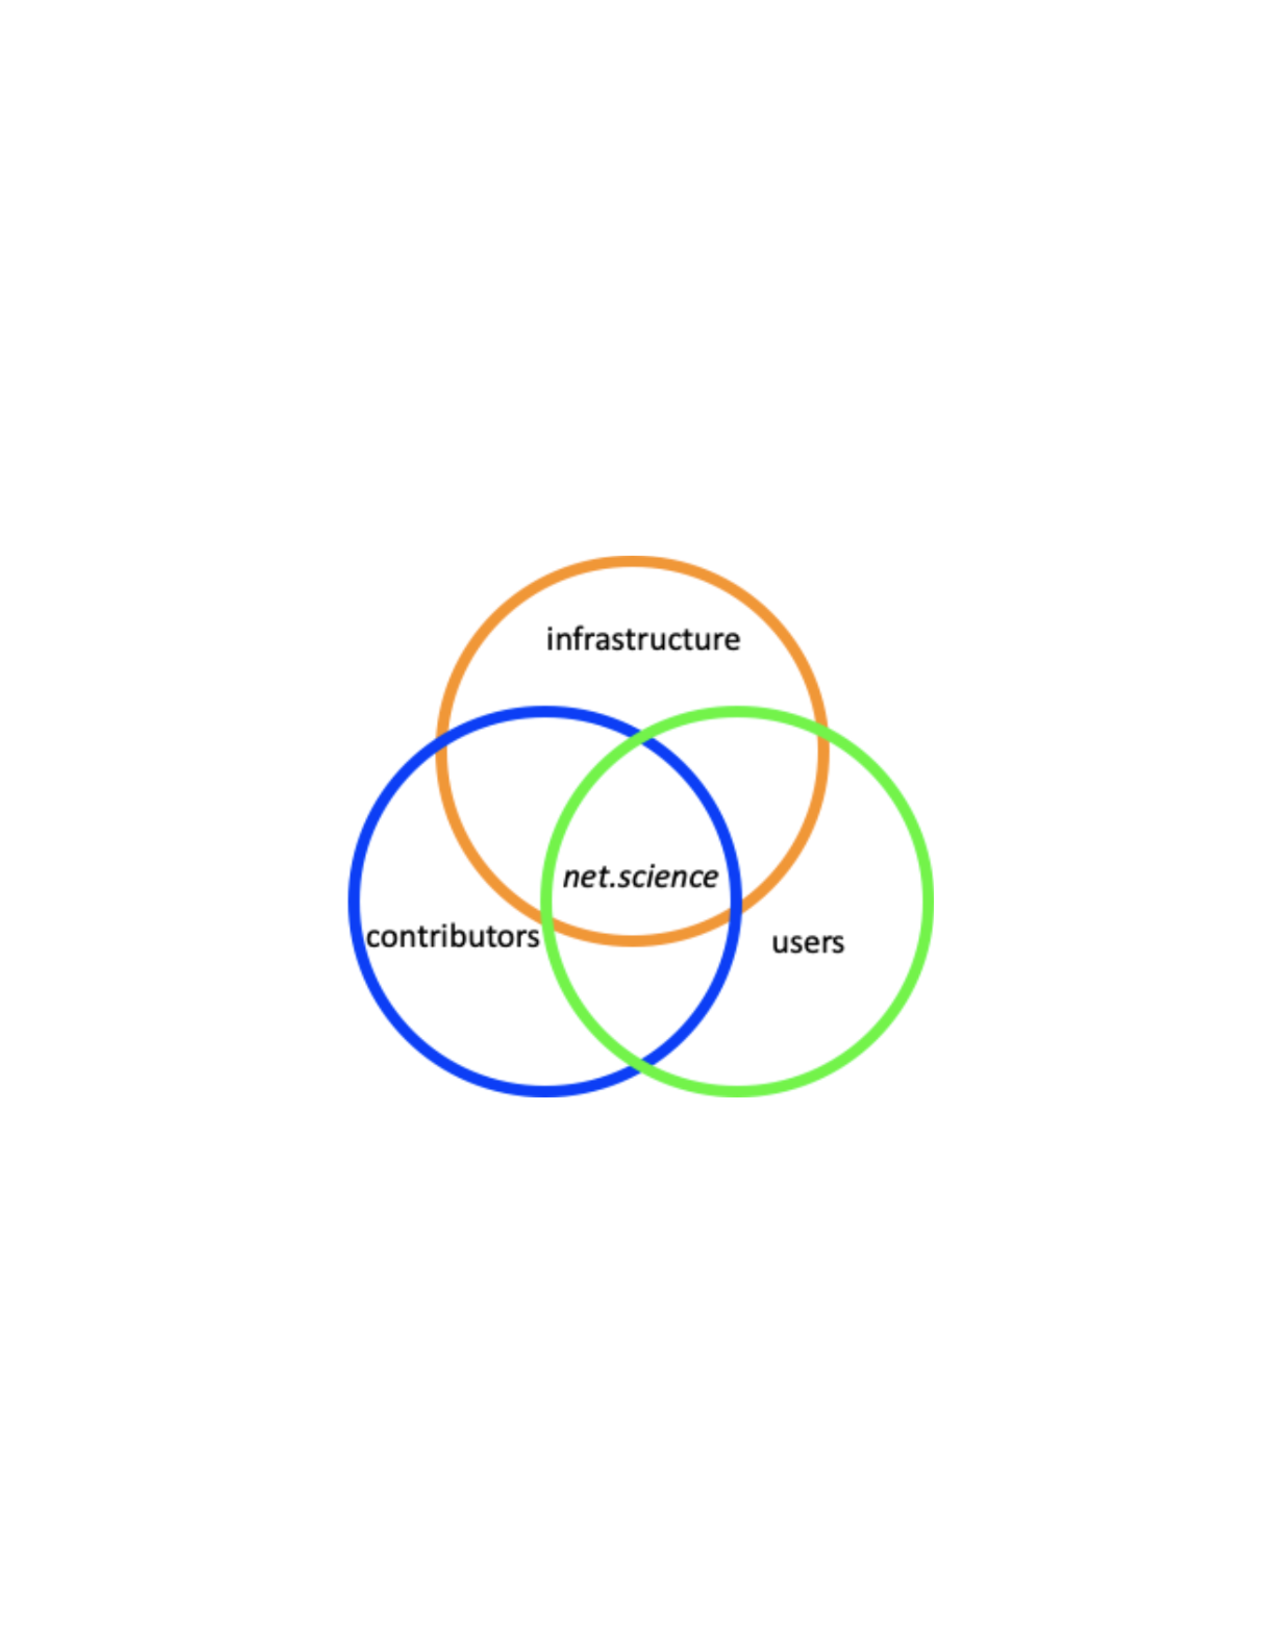
\includegraphics[scale=0.23]{figures/motivation.pdf}
\end{minipage}

\begin{itemize}[leftmargin=*,noitemsep,topsep=0pt]
\item Cyberinfrastructures (CIs)
	\begin{itemize}
	\item Network operations are similar across domains
	\item No existing general purpose network focused CI
	\item Existing CIs
	\begin{itemize}
	    \item XSEDE science gateway - No network gateways
	    \item Science Gateways Community Institute - ~600 gateways - 15 have
	    particular network analyses in narrow scope
	\end{itemize}
	\end{itemize}
\end{itemize}
\vspace*{0.2in}
}

\headerbox{System Description}
          {name=system,column=0,row=1,below=motive}{

\begin{minipage}{.5\textwidth}
\begin{itemize}[leftmargin=*,noitemsep,topsep=0pt]
\item Open access/Open source cyberinfrastructure \smallskip
\item General purpose network science \smallskip
\item Community resource \smallskip
\item Requires no software experience \smallskip
\item Usable by domain experts \smallskip
\item Under active development
\end{itemize}
\end{minipage}
\hfill
\begin{minipage}{.5\textwidth}
\begin{center}
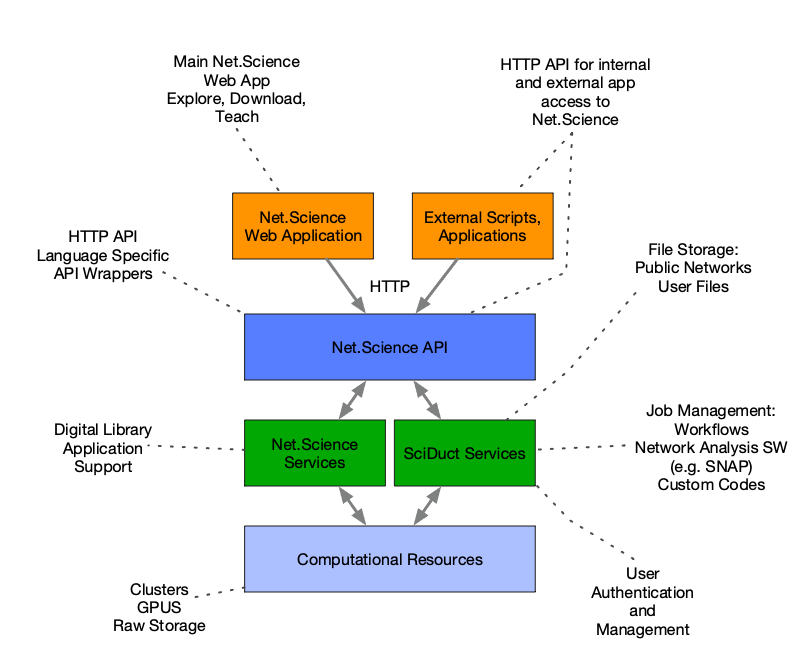
\includegraphics[scale=0.22]{figures/sys_descr.png}
\end{center}
\end{minipage}
\vspace*{0.2in}
}

\headerbox{Networks}
          {name=network,column=0,row=2,below=system}{         

\begin{minipage}{.5\textwidth}
\begin{center}
\textcolor{blue}{\textbf{Labeled Multigraph}}
\end{center}
\vspace{3mm}

\centering
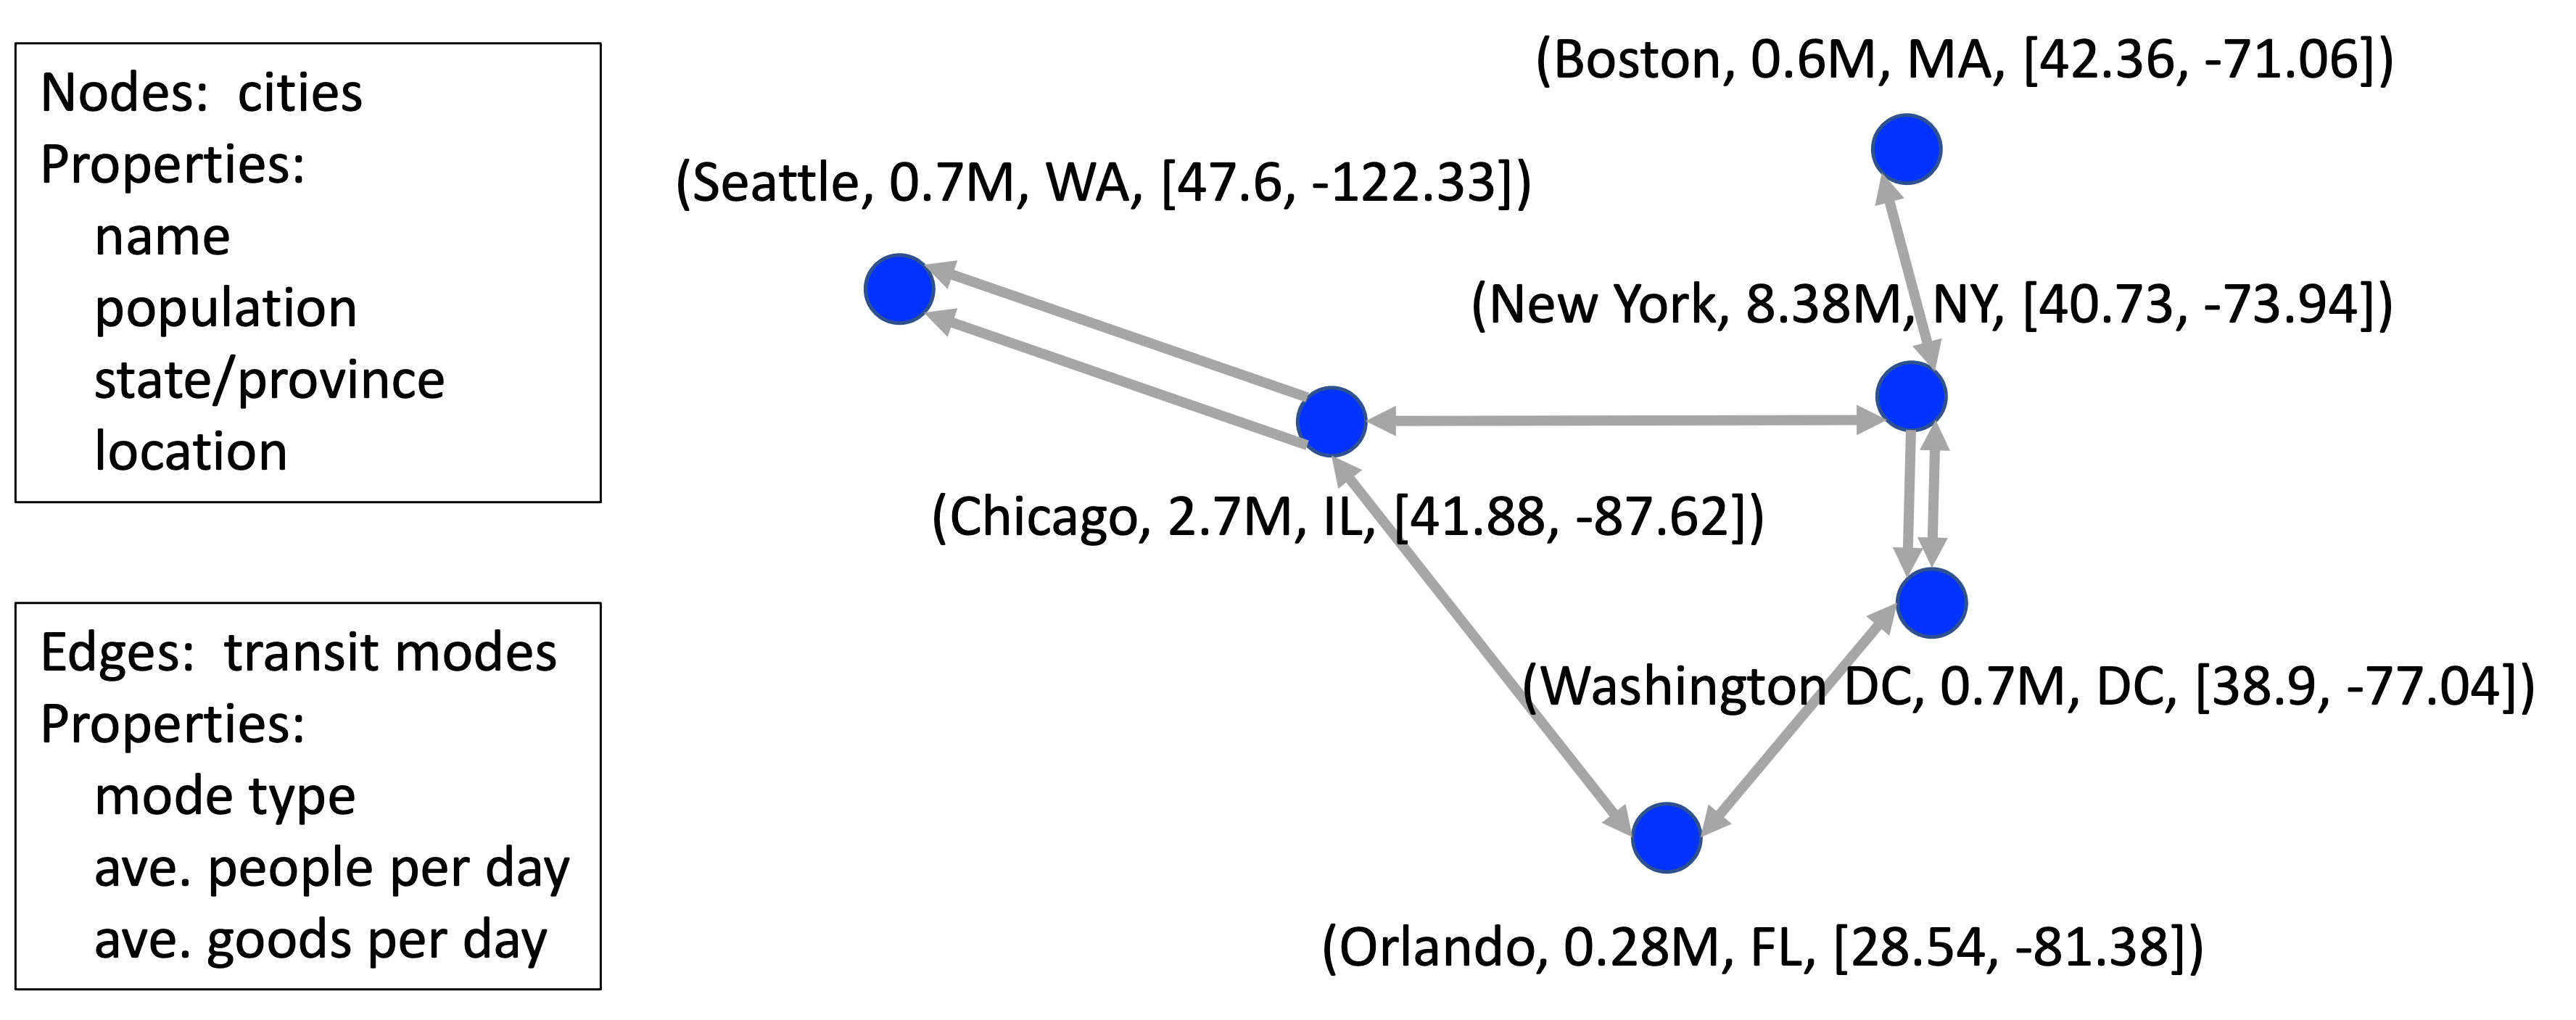
\includegraphics[scale=0.25]{figures/single_net.png}
%\captionof{figure}{Labeled Multigraph\label{label}}
\end{minipage}
\hfill
 \begin{minipage}{.35\textwidth}   
 \textcolor{blue}{\textbf{Multiplex Network}}
 % Multiplex Network
 \vspace{3mm}
 
 \centering
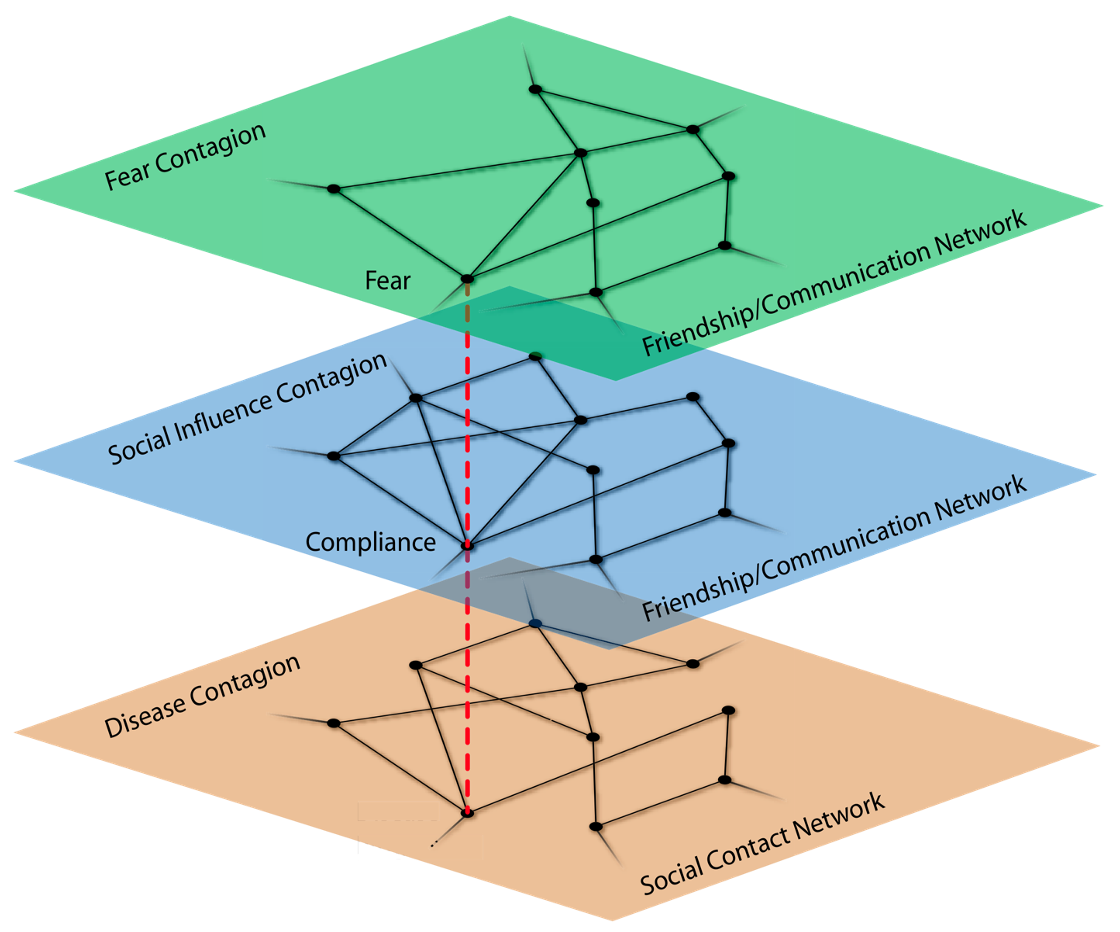
\includegraphics[scale=0.35]{figures/multi_net.png}
%\captionof{figure}{Multiplex Network\label{multiplex}}
\end{minipage}
\vspace*{0.2in}
}


\headerbox{Available Tasks}
          {name=services,column=0,row=1 ,below=network}{
\begin{minipage}[t]{0.48 \textwidth}
%\textbf{Implemented} ($\approx$ 200 total)   \smallskip
\textcolor{blue}{\textbf{Implemented ($\approx$ 200 total)}}
\medskip
\begin{itemize}[leftmargin=*,noitemsep,topsep=0pt]
    \item SNAP  \smallskip
    \item CSonNet   \smallskip 
    \item Plotting  \smallskip
    \item Apps to build networks  \smallskip
    \item Dynamical systems analyses
\end{itemize}
\end{minipage}
\quad
\begin{minipage}[t]{0.48 \textwidth}
%\textbf{In progress}
\textcolor{blue}{\textbf{In Progress}}\
  \medskip
\begin{itemize}[leftmargin=*,noitemsep,topsep=0pt]
    \item NetworkX    \smallskip
    \item Reliability polynomials    \smallskip
    \item SAT solvers    \smallskip
    \item Anomaly detection     \smallskip
    \item Apps to build networks    \smallskip
\end{itemize}
\end{minipage}
%\vspace*{0.1in}
}

%%%%%%%%%% Begin Column 1 %%%%%%%%%%

\headerbox{System Views}
          {name=sysViews, column=1,row=0}{

\begin{center}
\textcolor{blue}{\large\textbf{Task View}}
\end{center}
\begin{minipage}{.4\textwidth}
\begin{itemize}[leftmargin=*,noitemsep,topsep=0pt]
\item Tasks:
\begin{itemize}
    \item Graph operations
    \item Common services
    \item System support
\end{itemize}
\item Extensible
\end{itemize}
\end{minipage}
\hfill
\begin{minipage}{.6\textwidth}
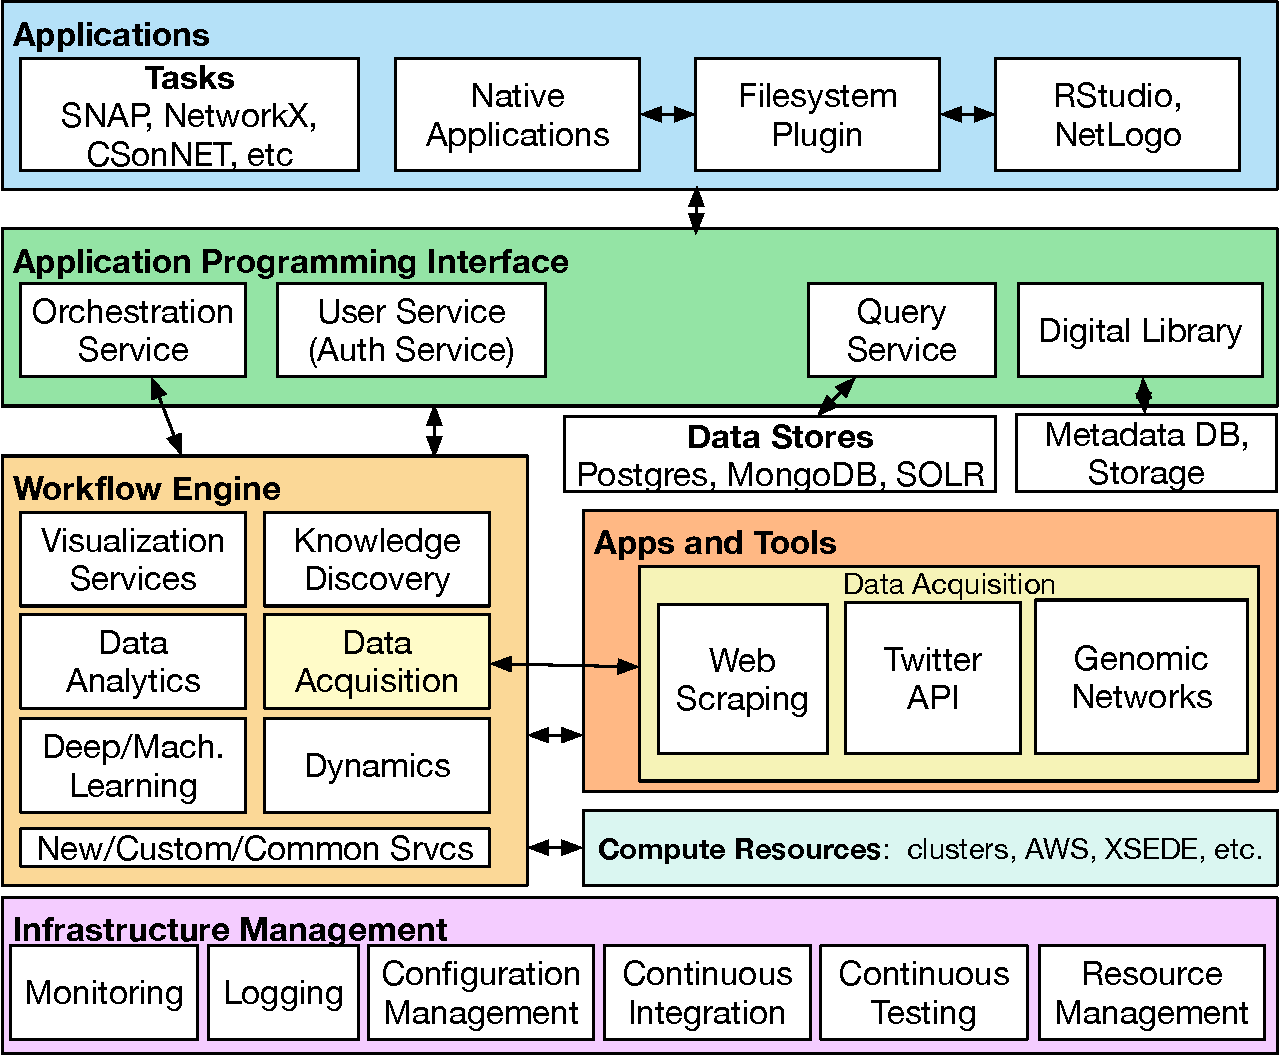
\includegraphics[scale=0.25]{figures/CINSArchV8.pdf} 
\end{minipage}

\vspace{4mm}

\begin{center}
\textcolor{blue}{\large\textbf{Process View}}
\end{center}
\vspace{-5mm}
\begin{minipage}{.24\textwidth}
\begin{itemize}[leftmargin=*,noitemsep,topsep=0pt]
\item Job submission via Web App \smallskip
\item 3rd party codes use same API \smallskip
\item Jobs currently run on a cluster
\end{itemize}
\end{minipage}
\qquad
\begin{minipage}{.73\textwidth}
\vspace{5mm}
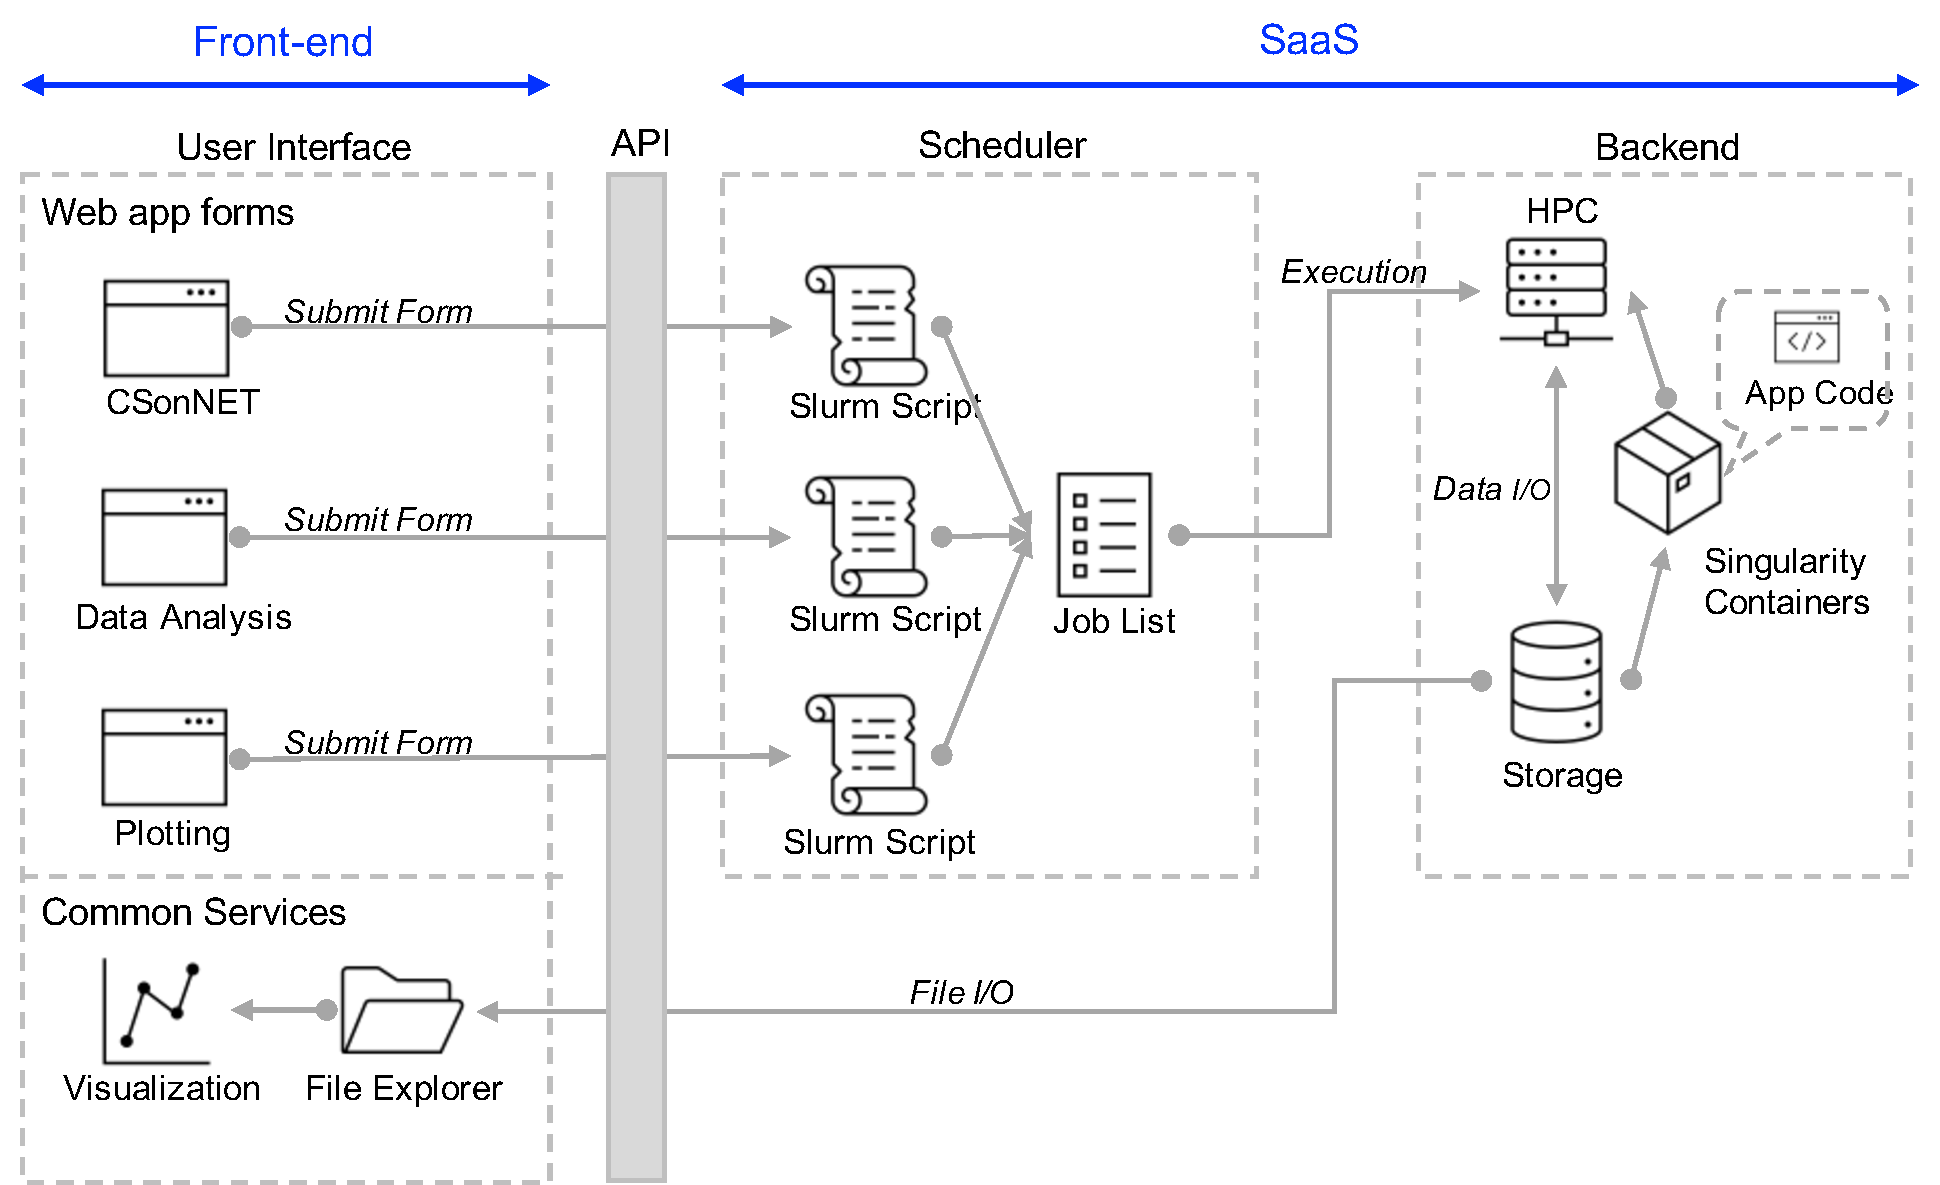
\includegraphics[scale=0.20]{figures/netsci_ops_v6.pdf}
\end{minipage}

}

\headerbox{Infrastructure (SciDuct)}
          {name=sciduct,column=1,row=1,below=sysViews}{
          
%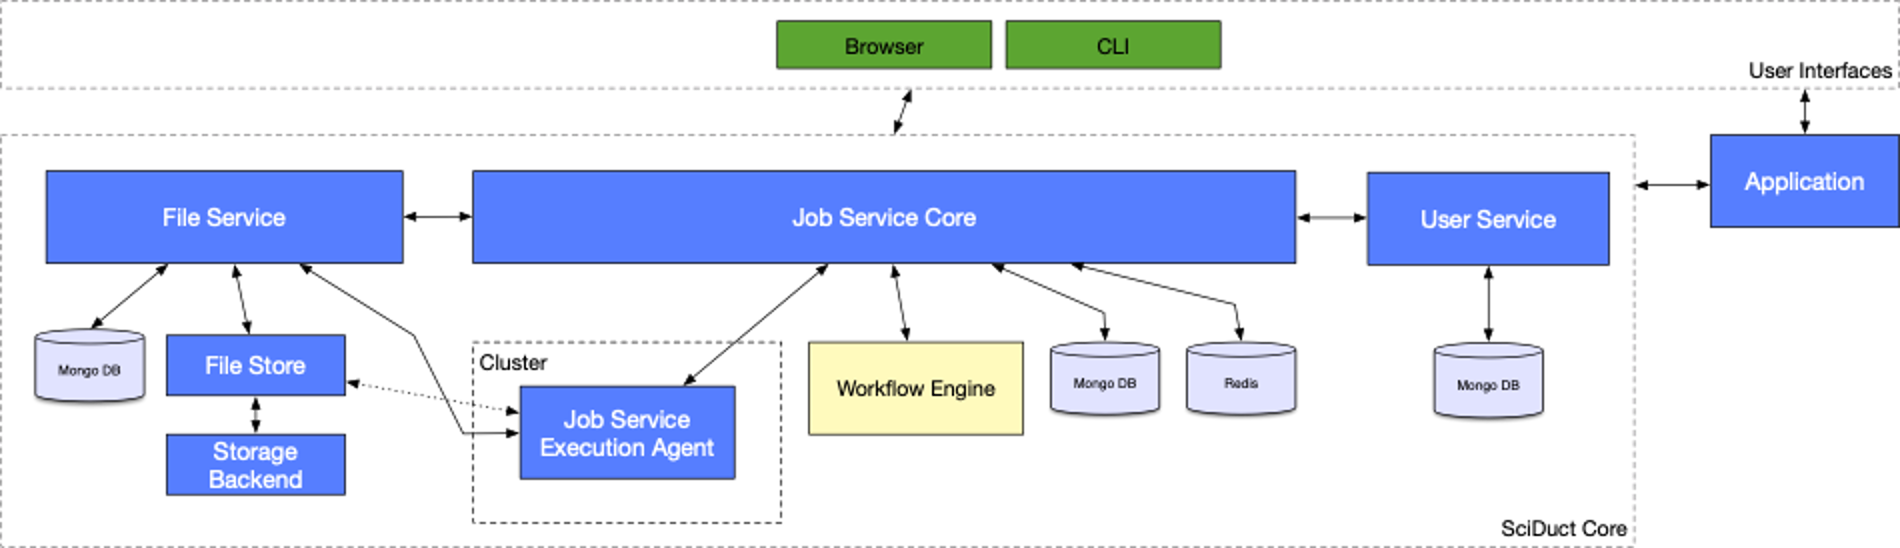
\includegraphics[scale=0.27]{figures/sciduct.png}
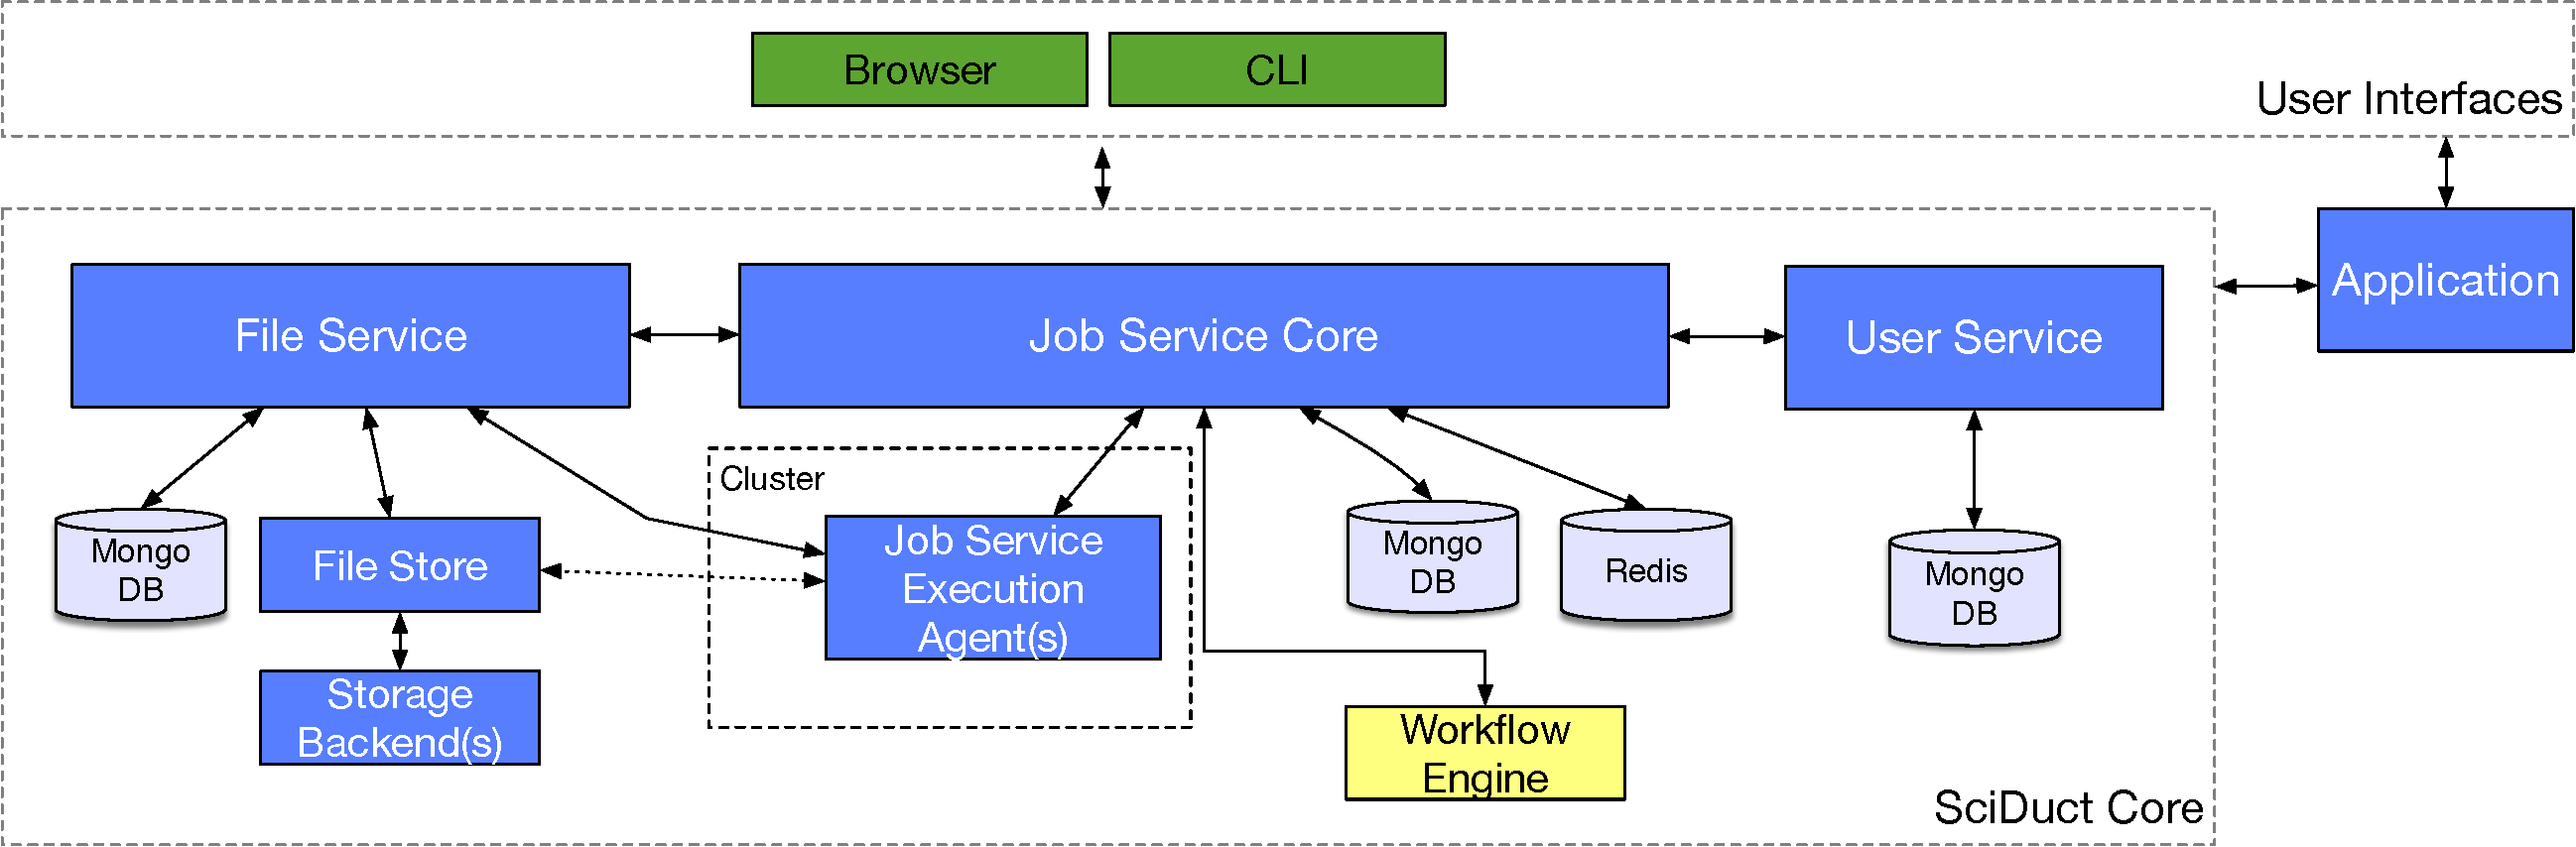
\includegraphics[scale=0.21]{figures/SciDuctComponents_legacy.pdf}


\vspace{5mm}
\noindent 
\begin{minipage}[t]{0.32\columnwidth}
User Service

\begin{itemize}[leftmargin=*,noitemsep,topsep=0pt]
	\item Authentication
	\item Teams
	\item Preferences
\end{itemize}
\end{minipage}
\hfill
\noindent
\begin{minipage}[t]{0.32\columnwidth}
File Service (FS)

\begin{itemize}[leftmargin=*,noitemsep,topsep=0pt]
	\item Data stores
	\item File validations
	\item Query system
\end{itemize}

\end{minipage}
\hfill
\noindent
\begin{minipage}[t]{0.32\columnwidth}
Job Service
\begin{itemize}[leftmargin=*,noitemsep,topsep=0pt]
	\item Task executor
	\item Manages FS I/O
	\item Container-based 

\end{itemize}

\end{minipage}
}


%\headerbox{Containerization}
%          {name=contain,column=1,row=2,below=sciduct}{
%          
%% 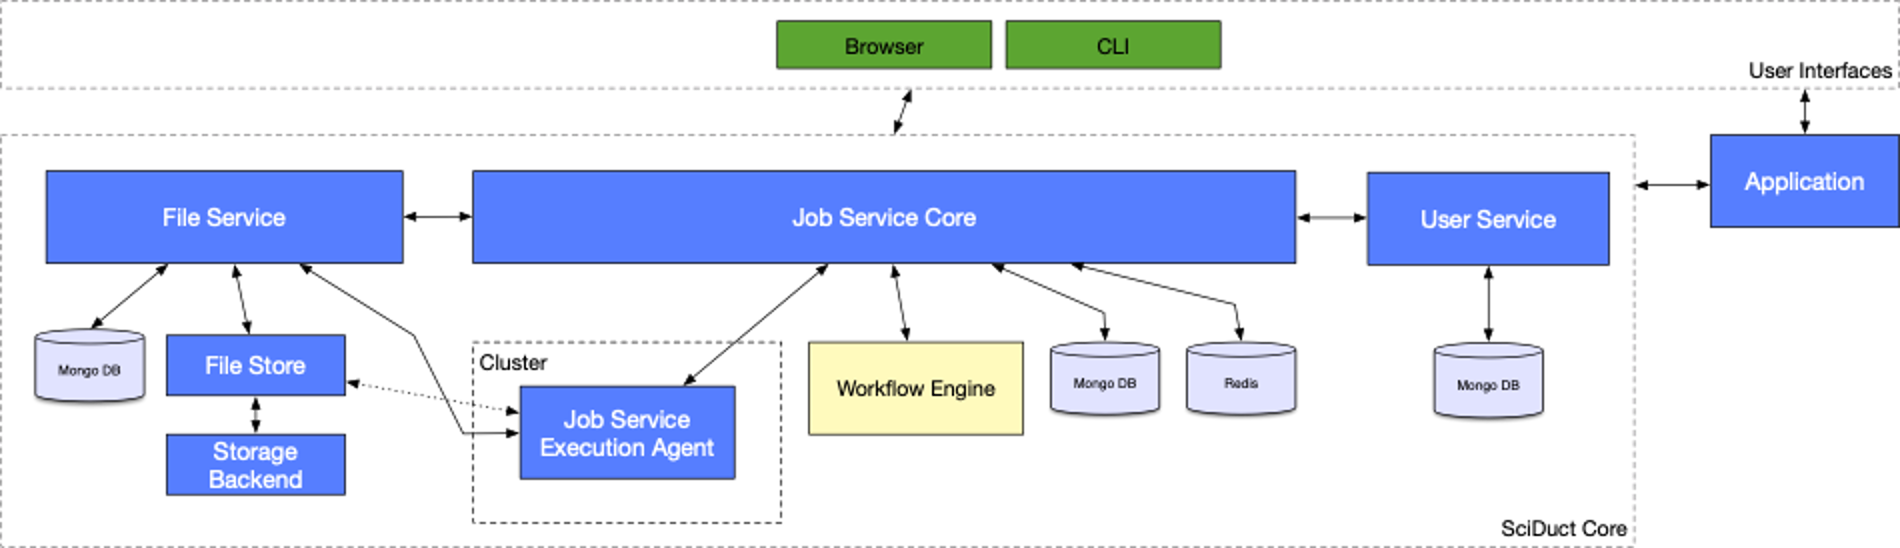
\includegraphics[scale=0.3]{figures/sciduct.png}
%%something on containerization
%\begin{minipage}{.5\textwidth}
%\begin{itemize}[leftmargin=*,noitemsep,topsep=0pt]
%\item Well-defined code invocations\newline from different environments \smallskip
%\item Portable \smallskip
%\item Self contained \smallskip
%\item Secure
%\end{itemize}
%\end{minipage}
%\hfill
%\begin{minipage}{.5\textwidth}
%\begin{center}
%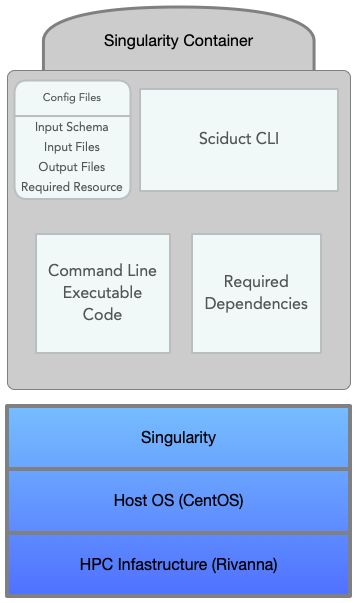
\includegraphics[scale=0.22, trim = 0in 2.77in 0in 0in, clip]{figures/container_figure_v02.png}
%\end{center}
%\end{minipage}
%} 

\headerbox{Get Involved}
          {name=contri,column=1,row=2 ,below=sciduct}{
\begin{itemize}[leftmargin=*,noitemsep,topsep=0pt]
\item We are looking for
\begin{itemize}
\item Data collection tools
\item Data on networks
\item Apps to build and analyze networks
\end{itemize}
\item Contributors given full credit in system.
\medskip
\item Questions?~ \textcolor{green}
        {\textbf{\texttt{net.science@virginia.edu}}}
\end{itemize}
\vspace*{0.1in}
}


%%%%%%%%%% Begin Column 2 %%%%%%%%%%

\headerbox{Web App}
          {name=frontend,column=2,row=0}{

\begin{center}
\textcolor{blue}{\large\textbf{Input Forms}}
\end{center}

\textbf{Contagion Simulation:}
% \medskip

\begin{center}
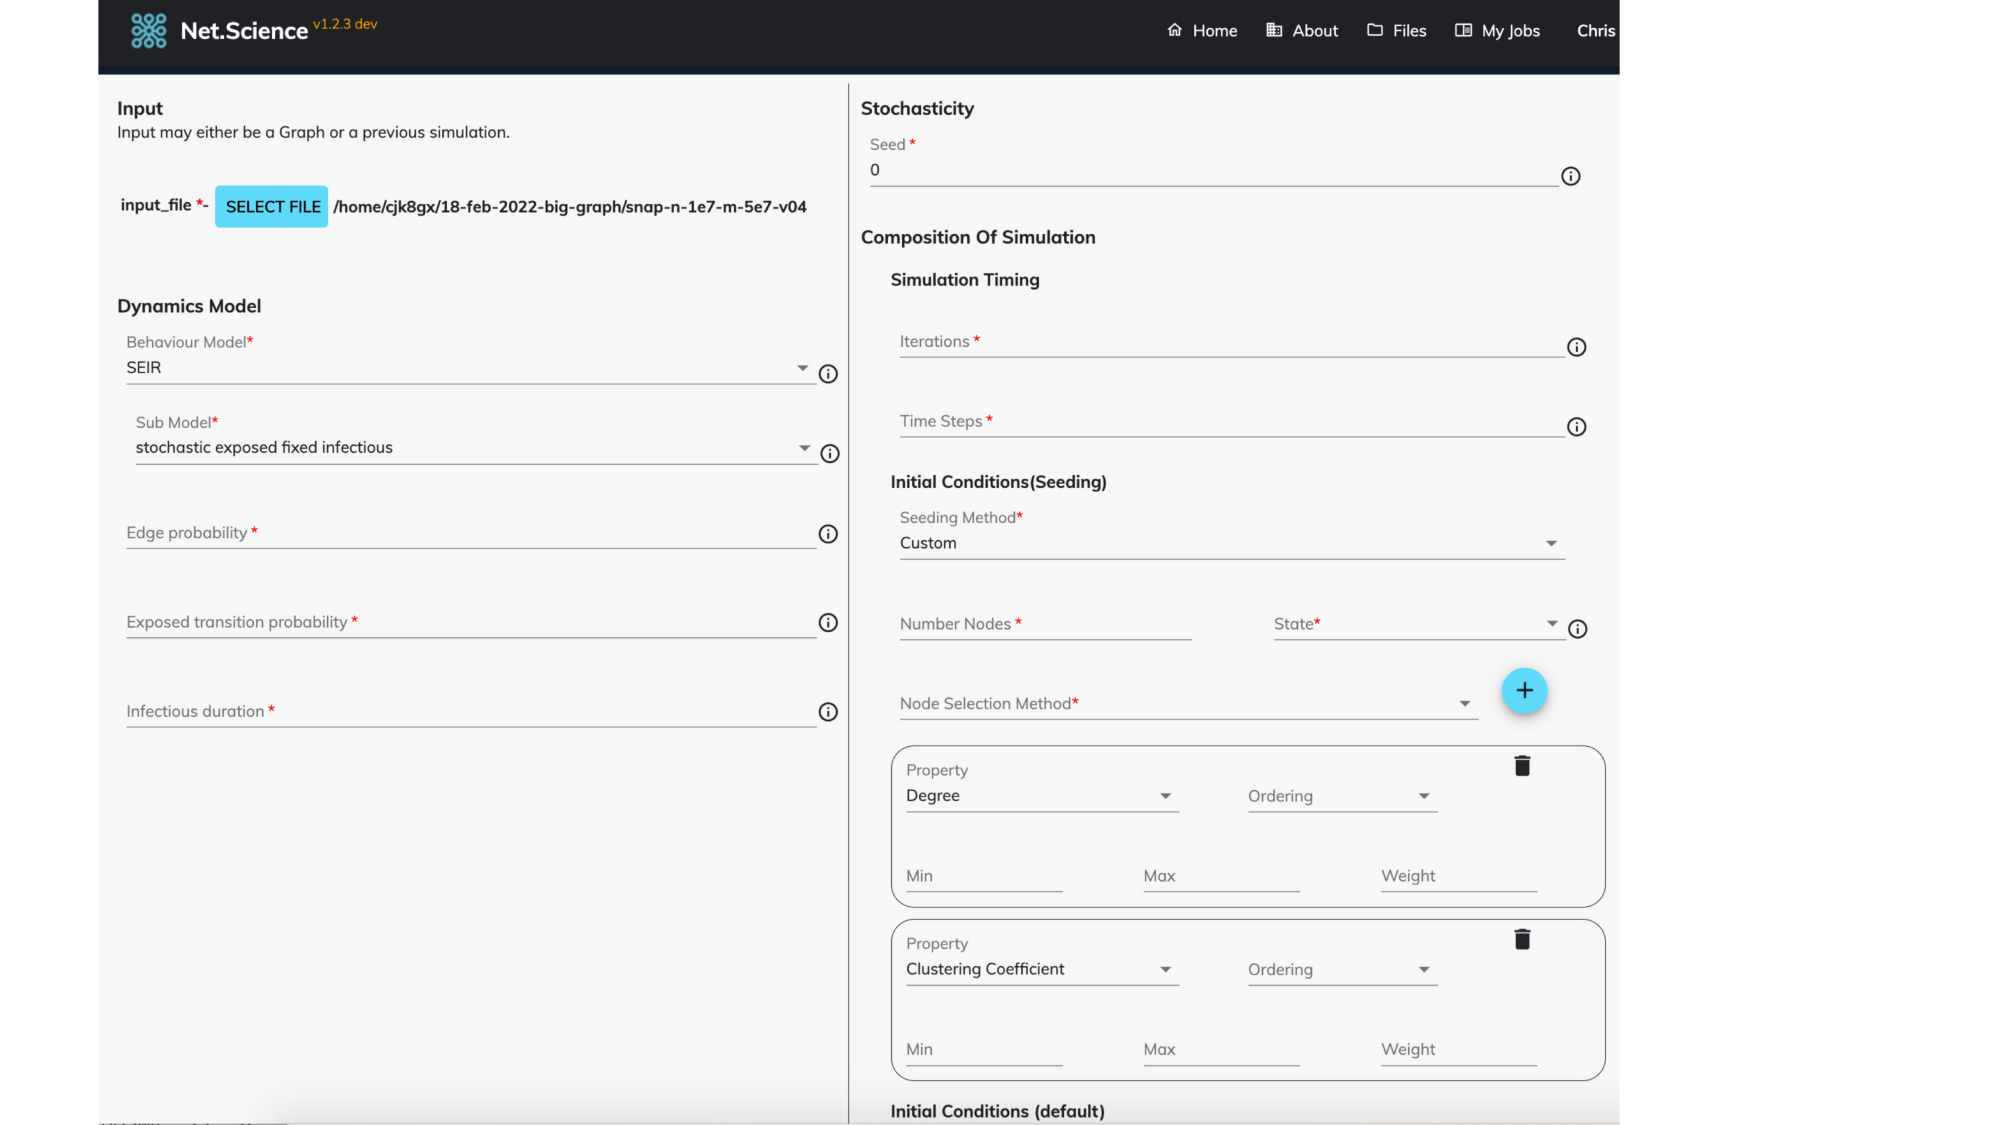
\includegraphics[scale=0.28]{figures/csonnet-model-seeds.pdf}
\end{center}

\textbf{Publication Quality Plot Generation:}
% \medskip

\begin{center}
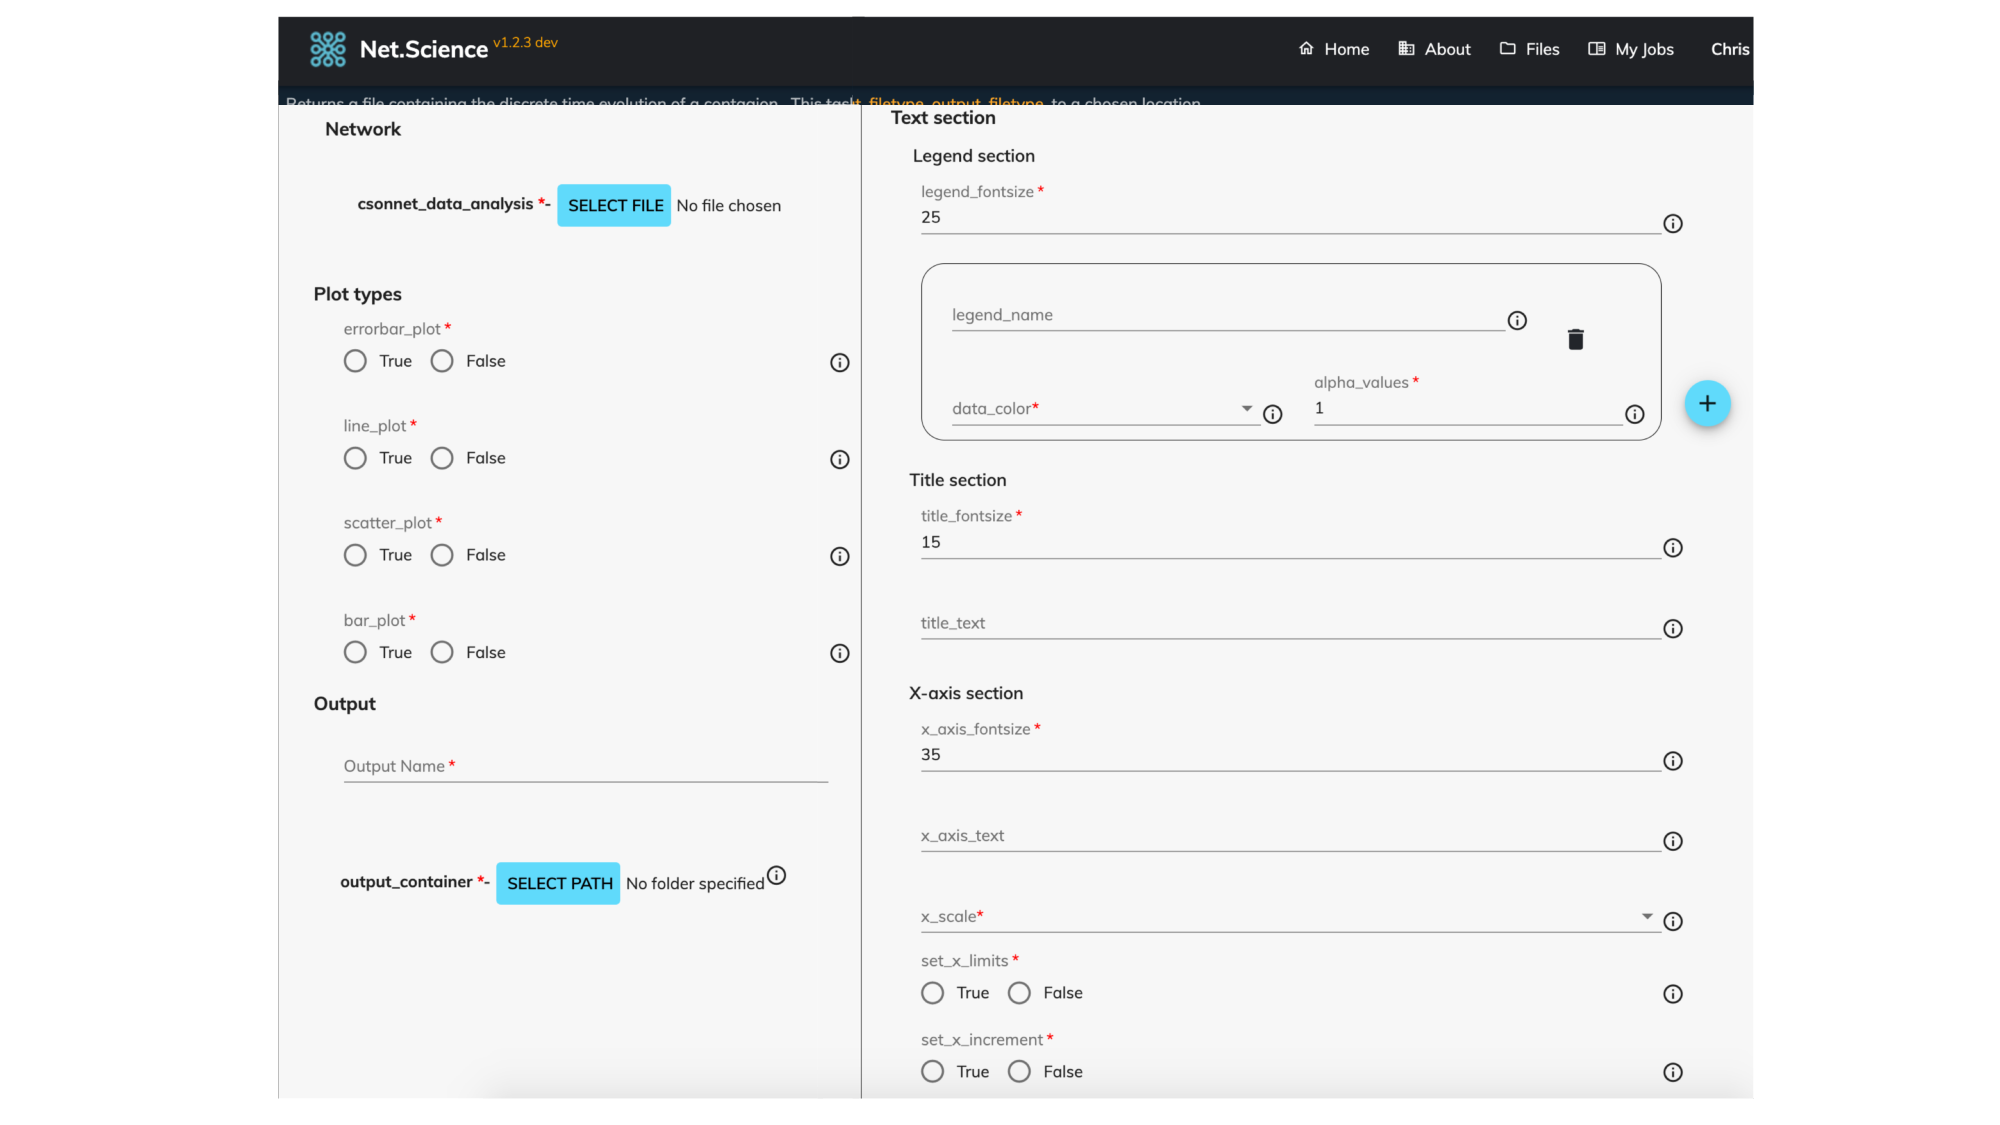
\includegraphics[scale=0.28]{figures/plot_input.pdf}
\end{center}


% \begin{minipage}{.29\textwidth}
% \begin{itemize}[leftmargin=*,noitemsep,topsep=0pt]
% \item Input form, contagion simulation
% \item Discrete time, propagation on networks
% \end{itemize}
% \end{minipage}
% \hfill
% \begin{minipage}{.71\textwidth}         
% 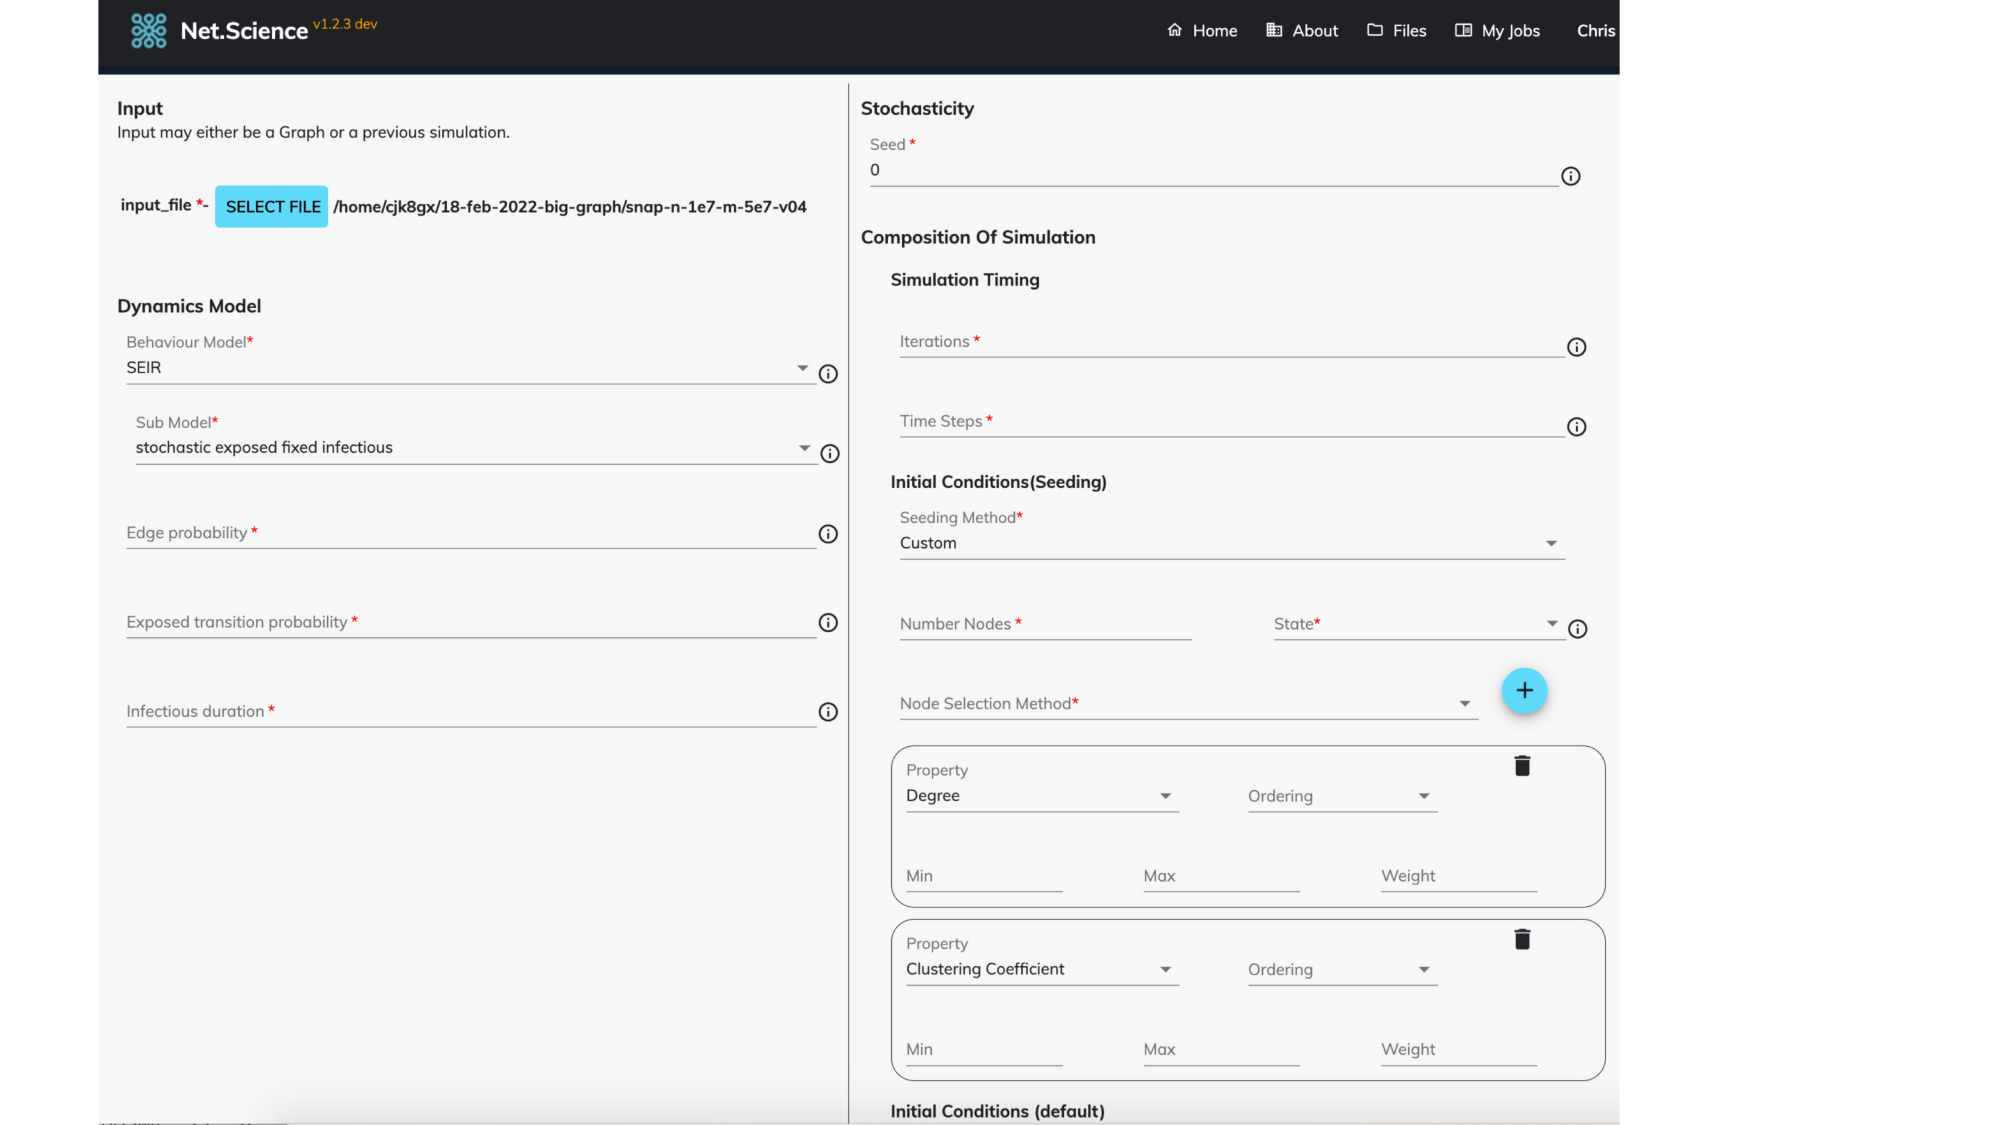
\includegraphics[scale=0.25]{figures/csonnet-model-seeds.pdf} 
% \end{minipage}

% \vspace{0.3in}

% \begin{minipage}{.29\textwidth}
% \begin{itemize}[leftmargin=*,noitemsep,topsep=0pt]
% \item Input form, plot generation
% \item Publication quality
% \end{itemize}
% \end{minipage}
% \hfill
% \begin{minipage}{.71\textwidth}  
% \vspace{5mm}
% 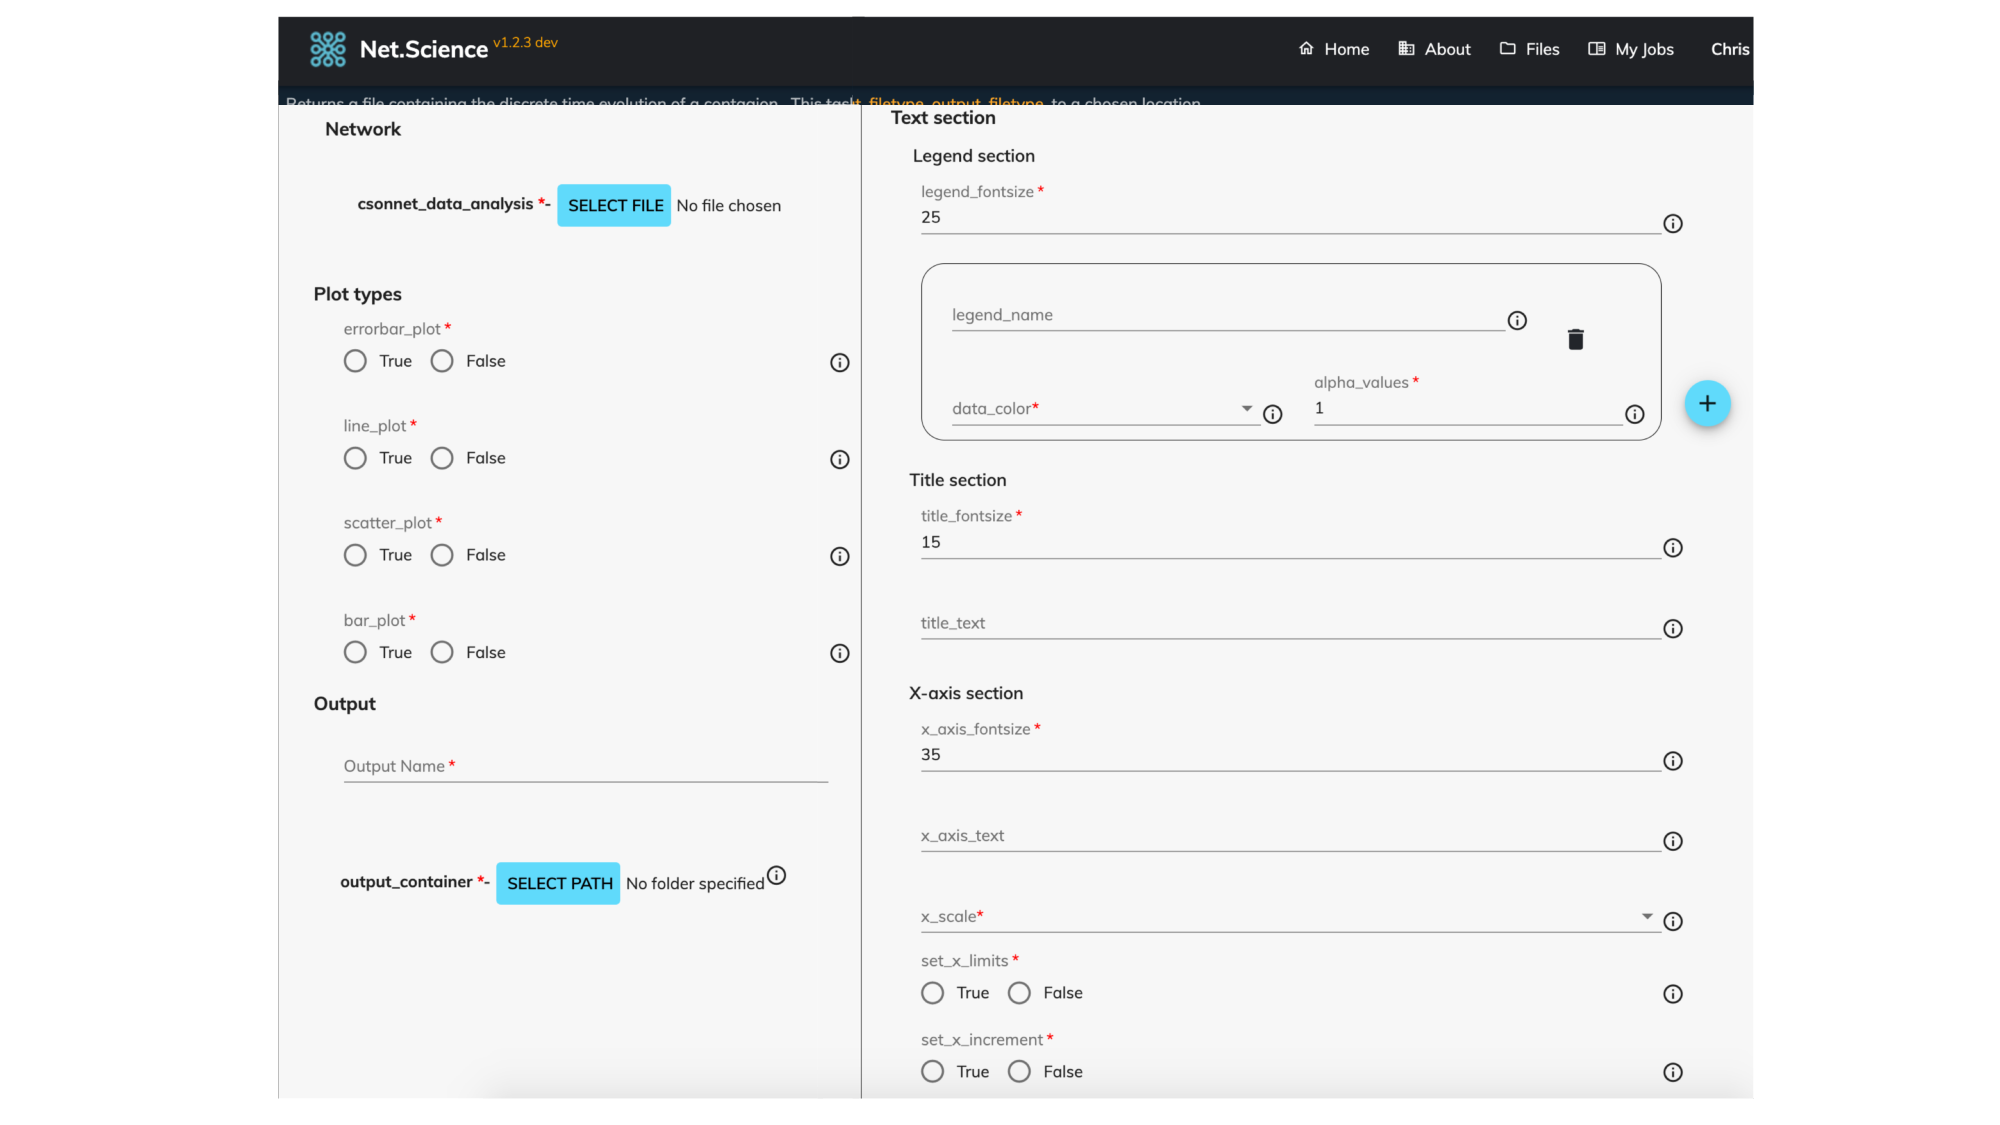
\includegraphics[scale=0.26]{figures/plot_input.pdf}
% \end{minipage}
% \hfill
% \vspace{5mm}

%\begin{minipage}{0.48\linewidth}
%Graph:  nodes and edge are those of graph
%
%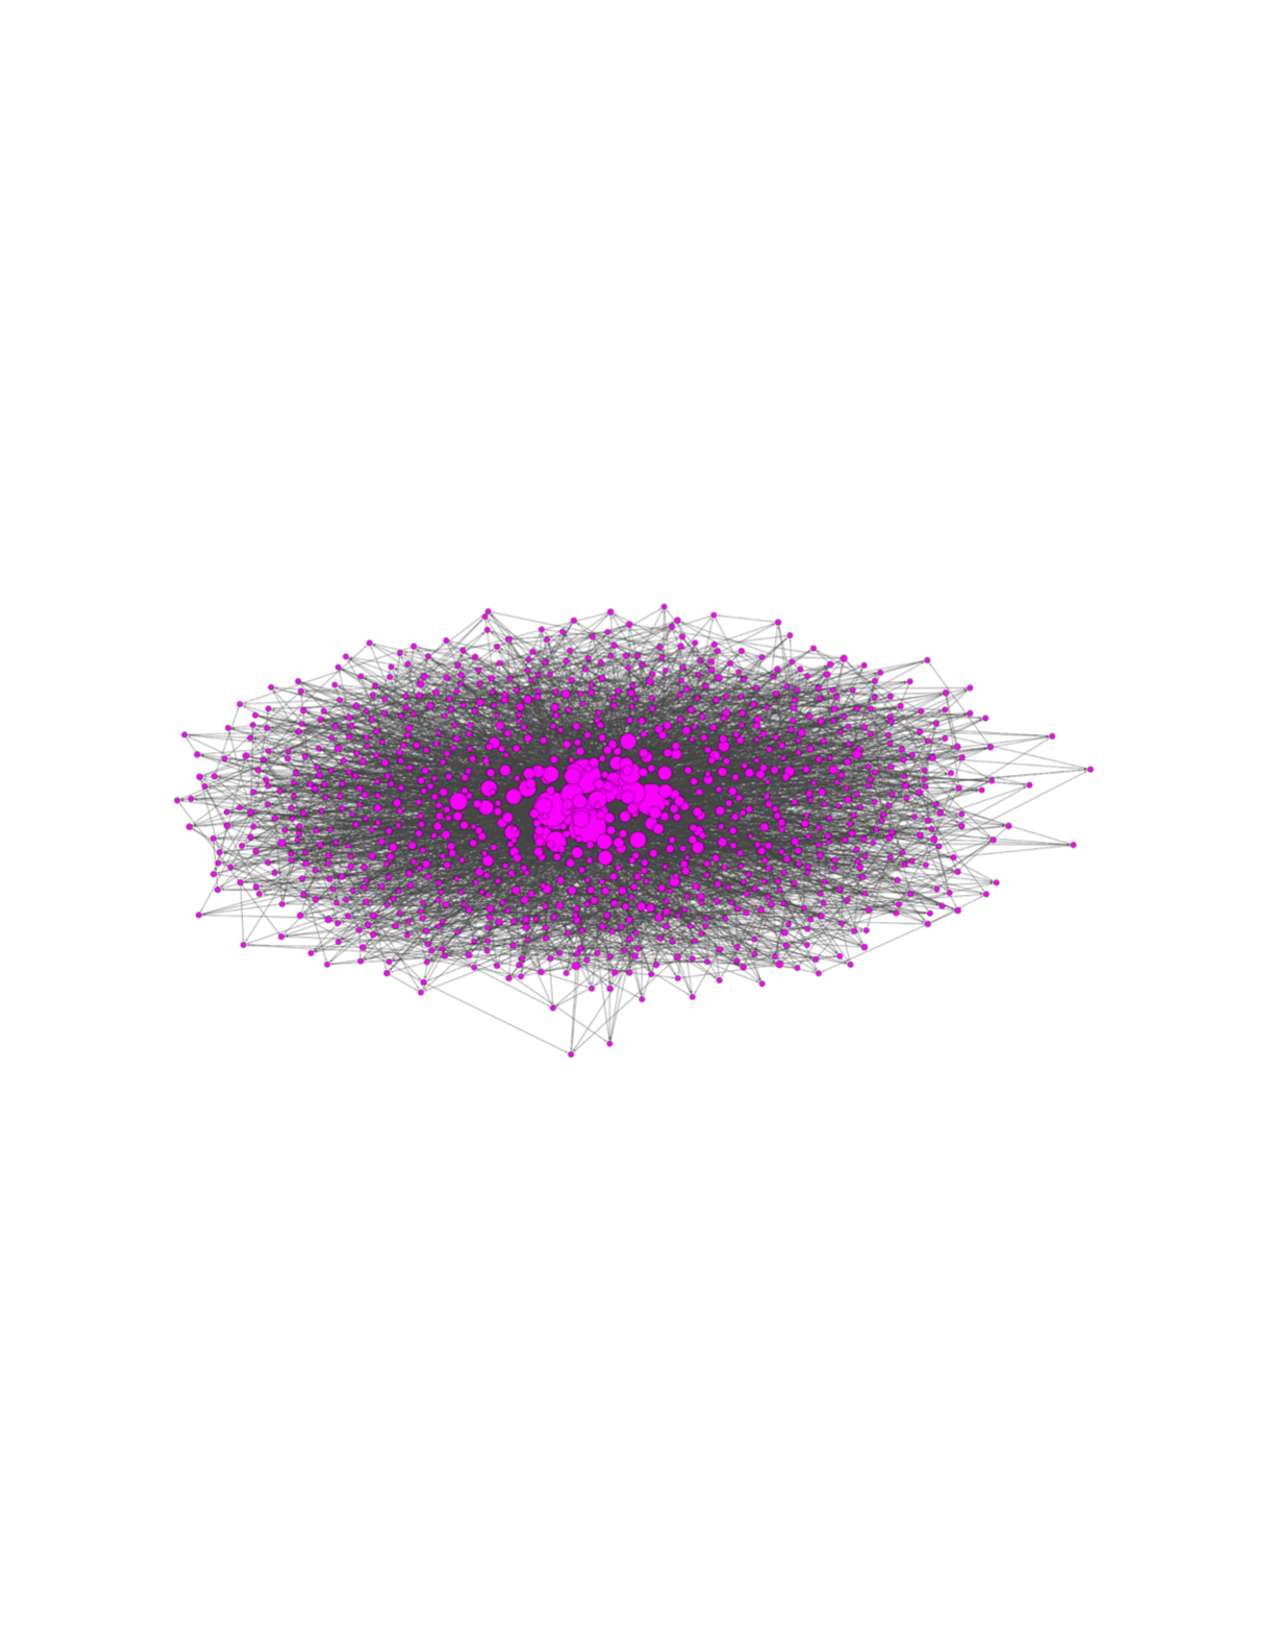
\includegraphics[scale=0.3]{figures/graph_nodes.pdf} 
%\end{minipage}
%\hfill
%\begin{minipage}{0.48\linewidth}
%
%Graph:  nodes are communities
%and edge are those of between communities
%
%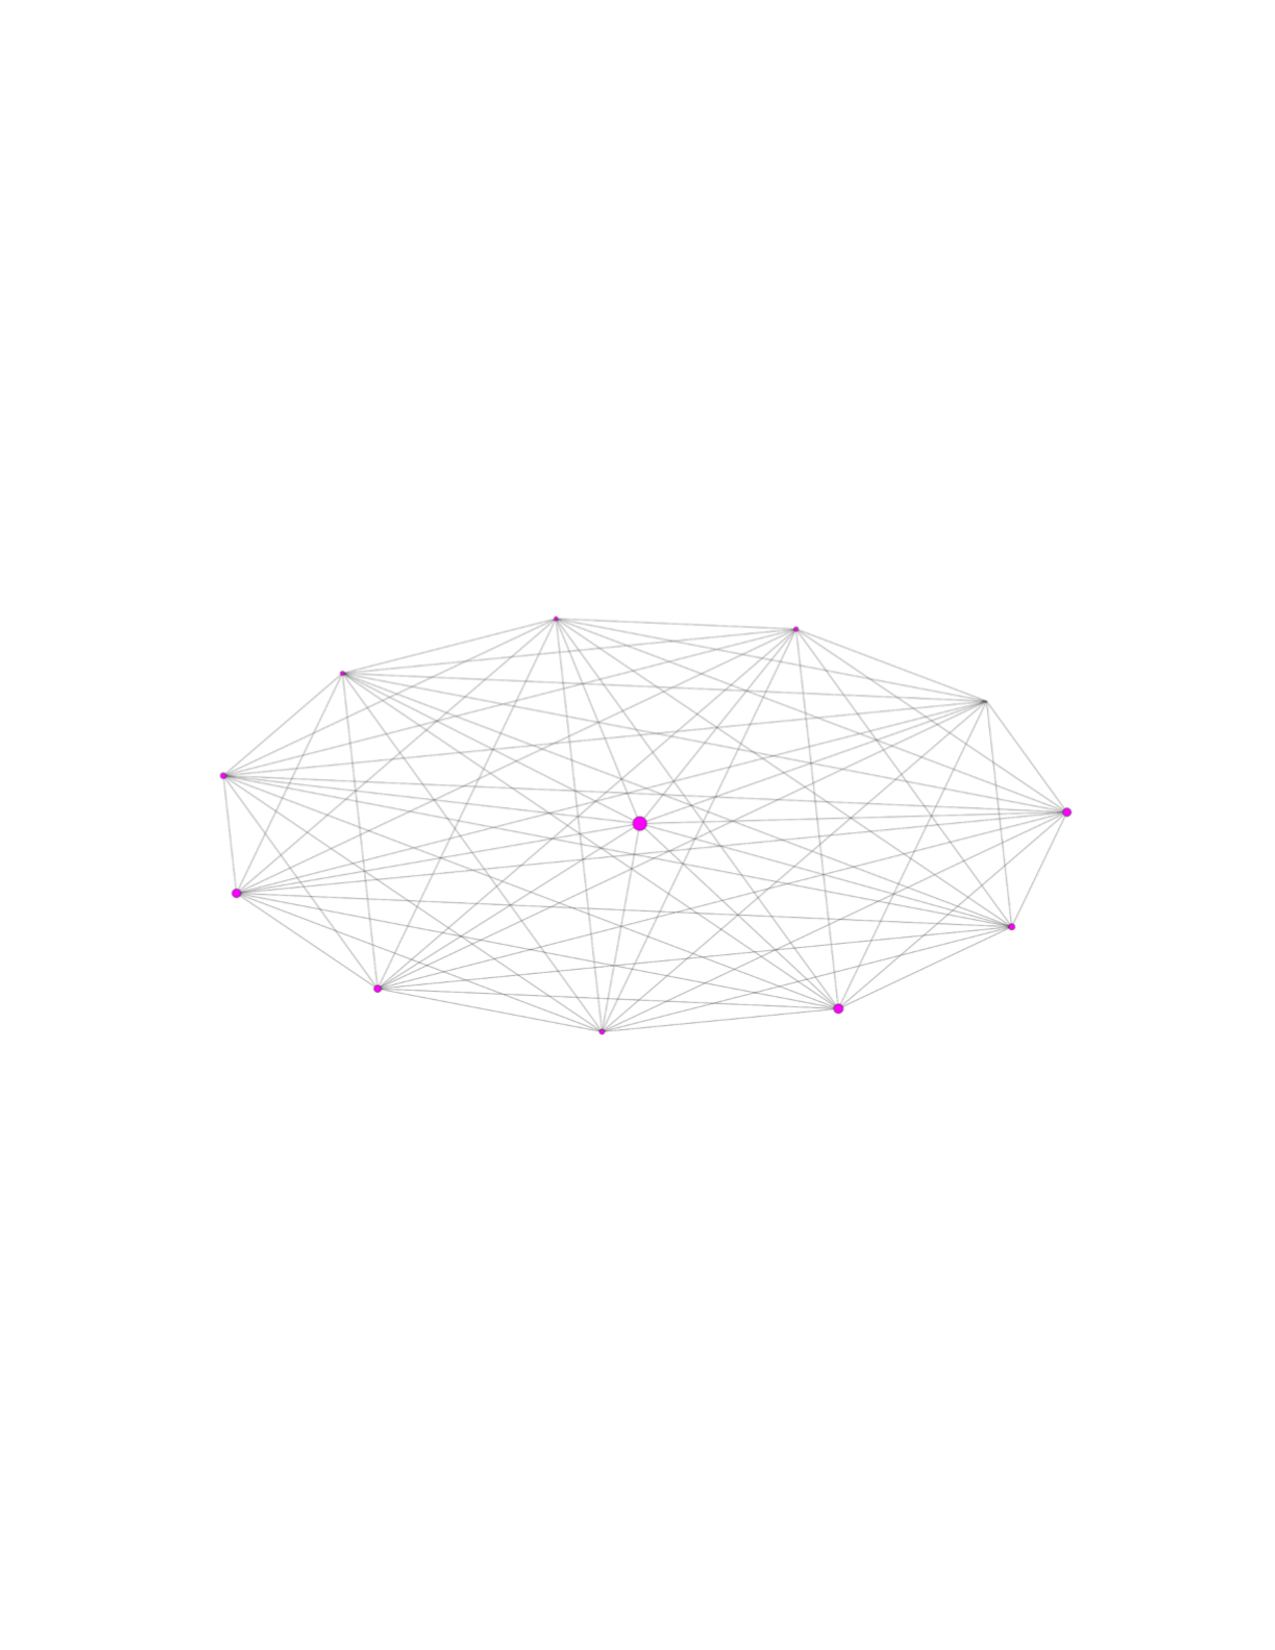
\includegraphics[scale=0.3]{figures/graph_community.pdf} 
%\end{minipage}

% \vspace{0.3in}

\begin{center}
\textcolor{blue}{\large\textbf{Outputs}}
\end{center}


Graph Visualizations

\begin{minipage}{0.3\linewidth}
% Graph:  nodes and edges are those of graph
%Uncontracted graph
%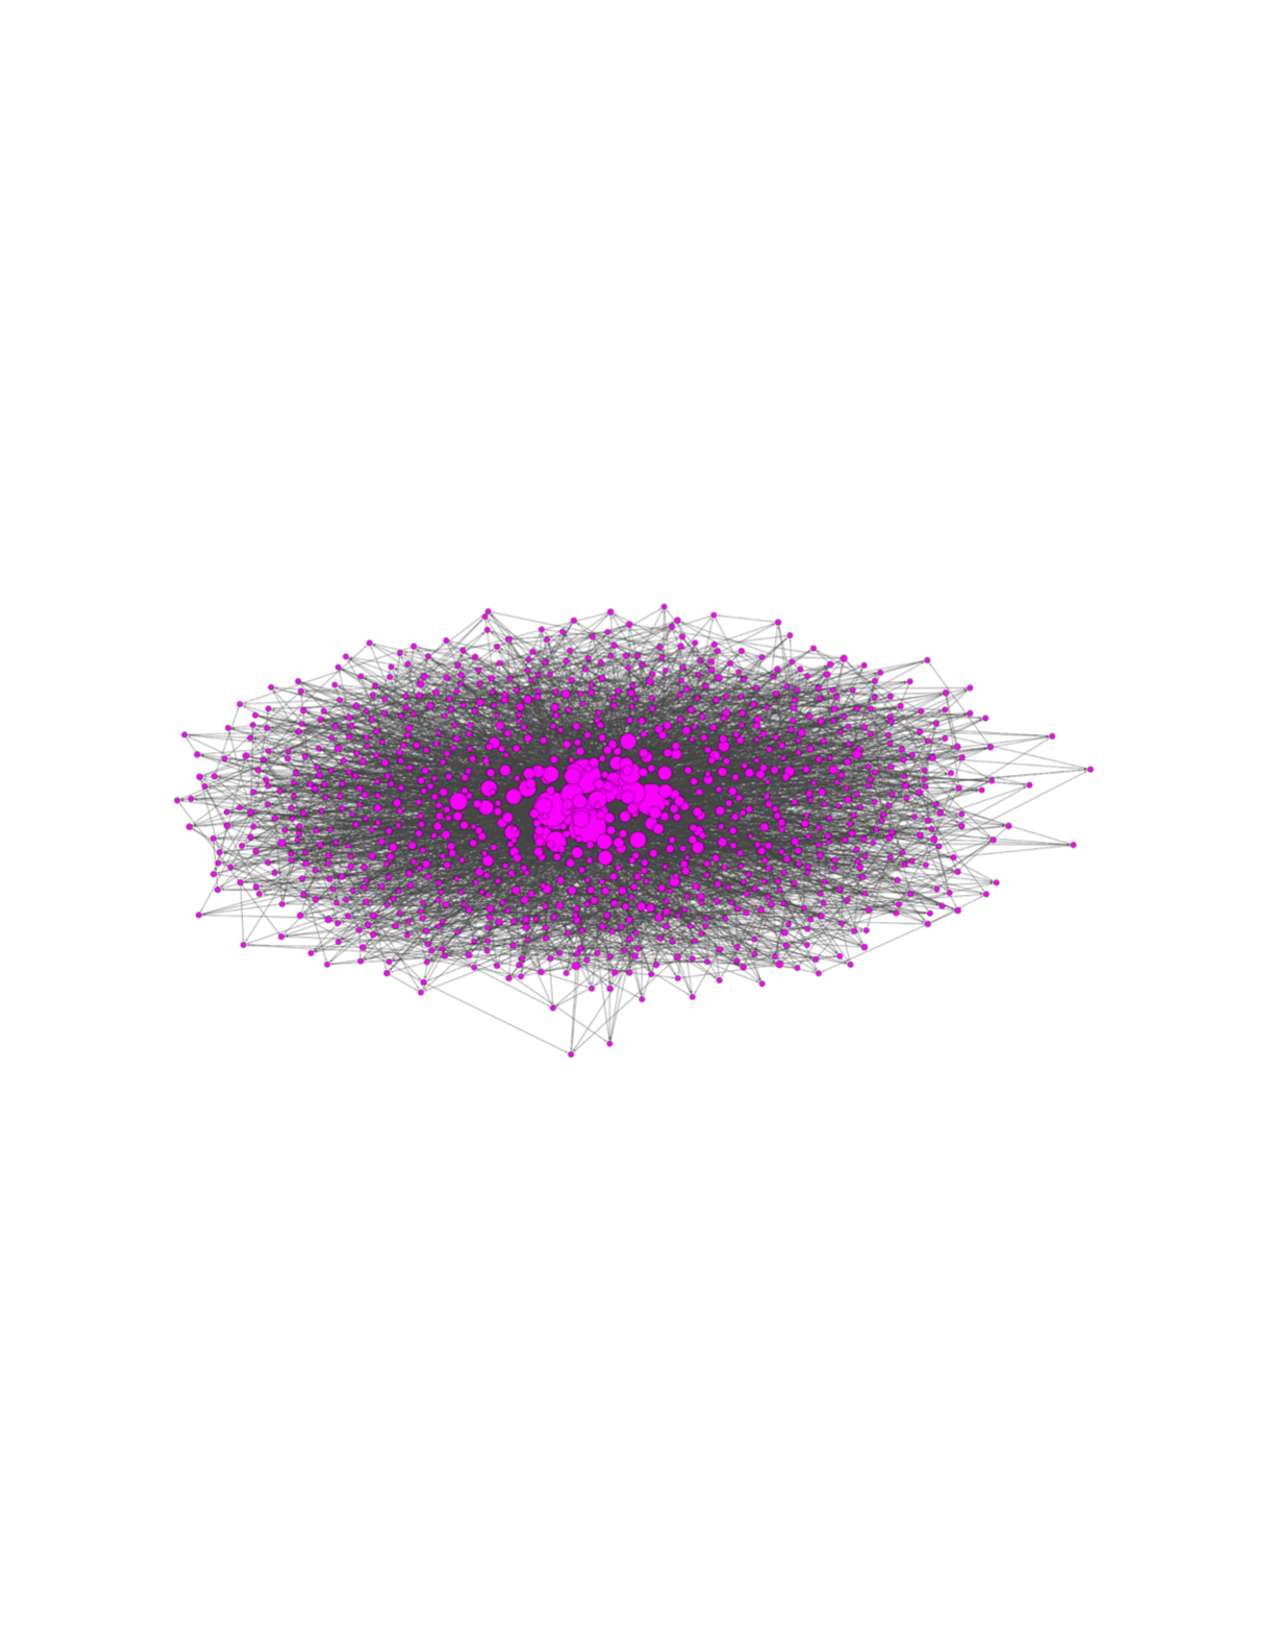
\includegraphics[scale=0.3]{figures/graph_nodes.pdf} 
%Contracted~graph
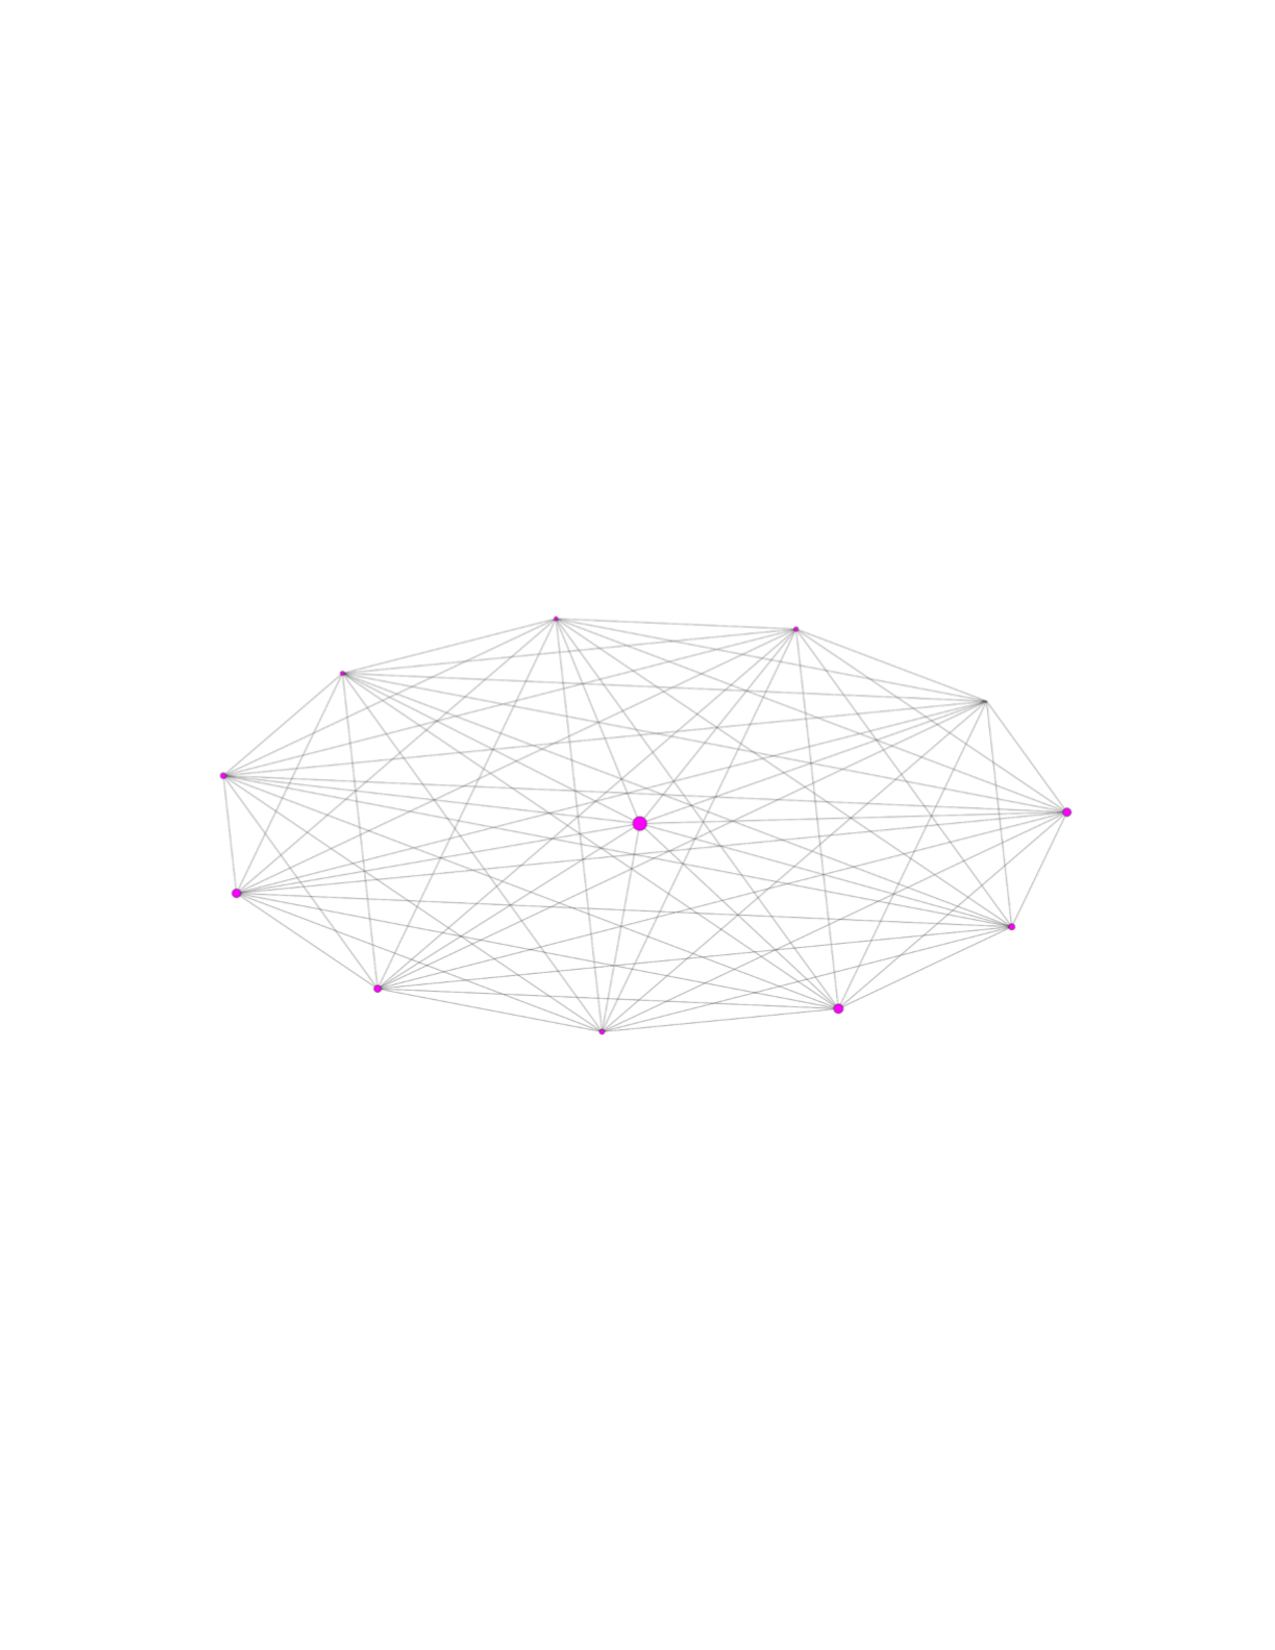
\includegraphics[scale=0.3]{figures/graph_community.pdf} 

\end{minipage}
\hfill
\begin{minipage}{0.3\linewidth}

%Contracted graph
%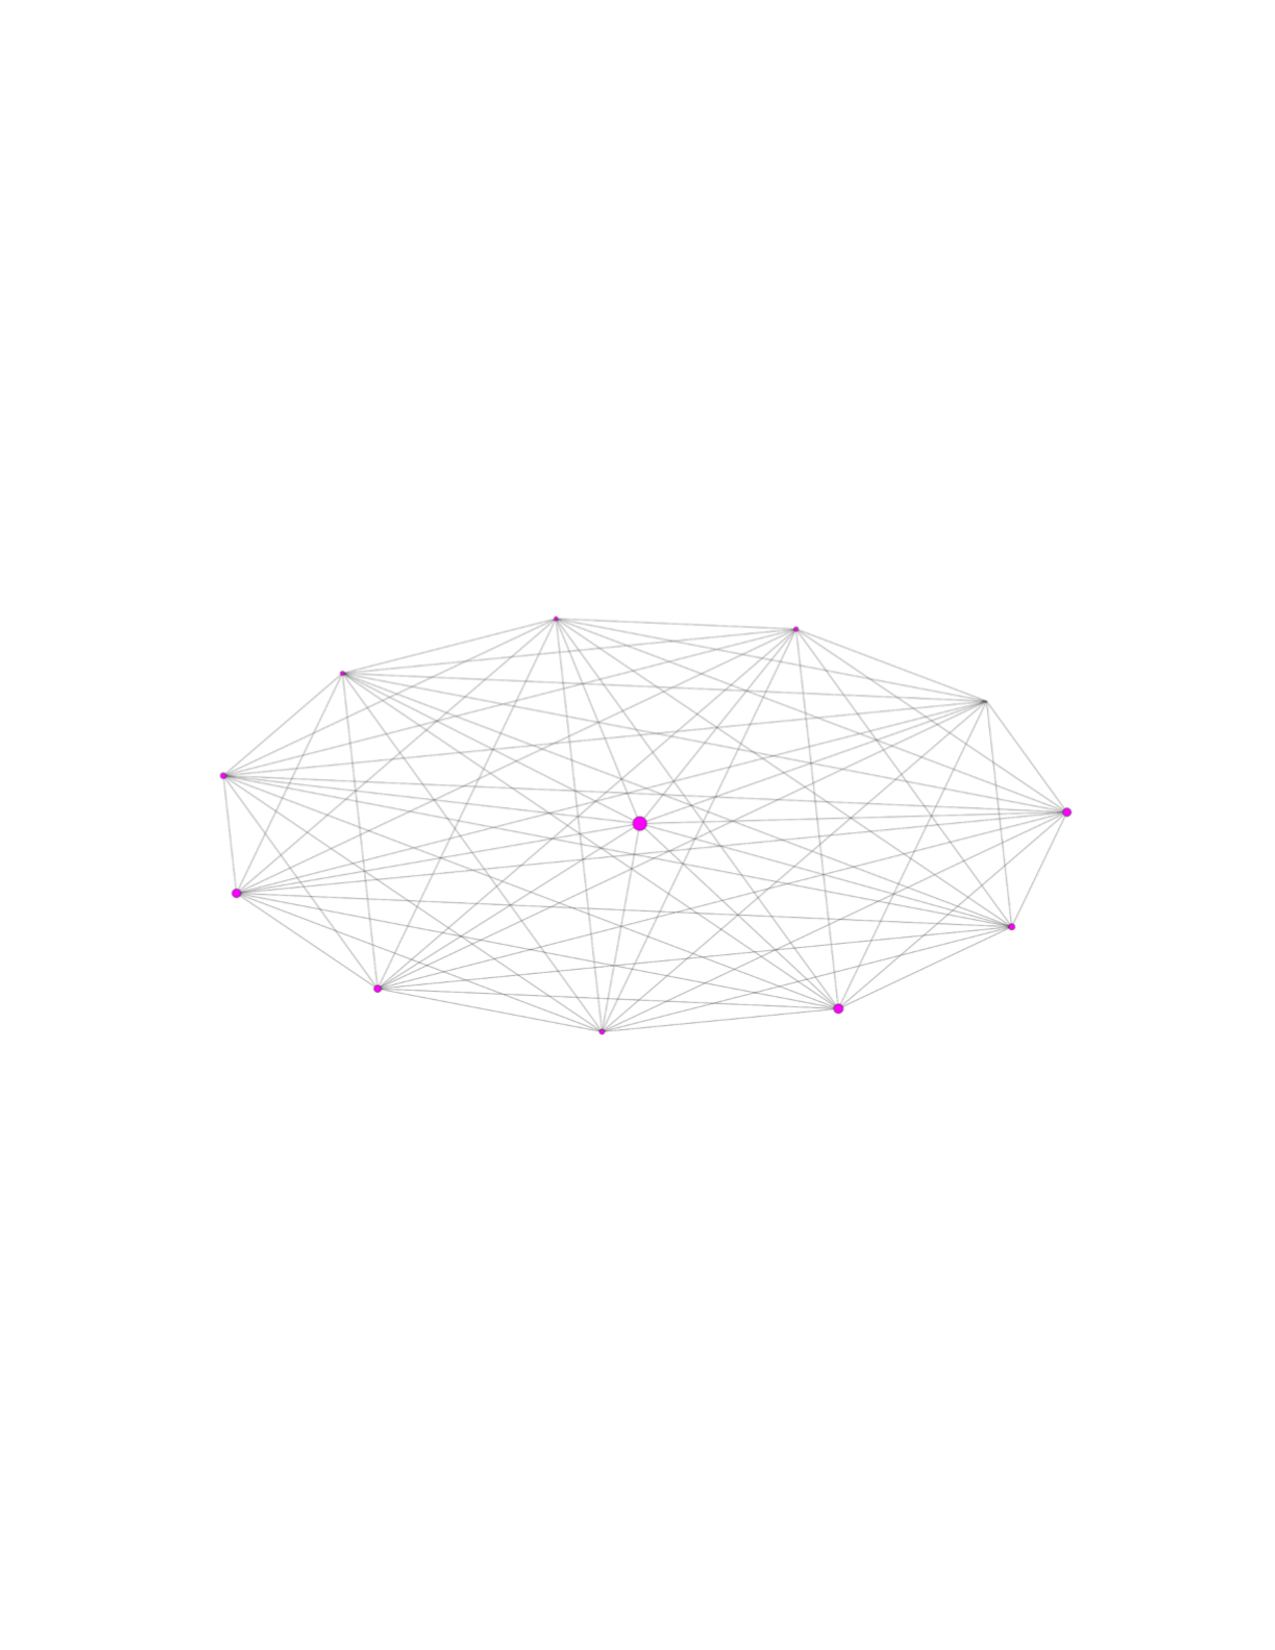
\includegraphics[scale=0.3]{figures/graph_community.pdf} 
%Uncontracted graph
\hspace*{-0.25in}
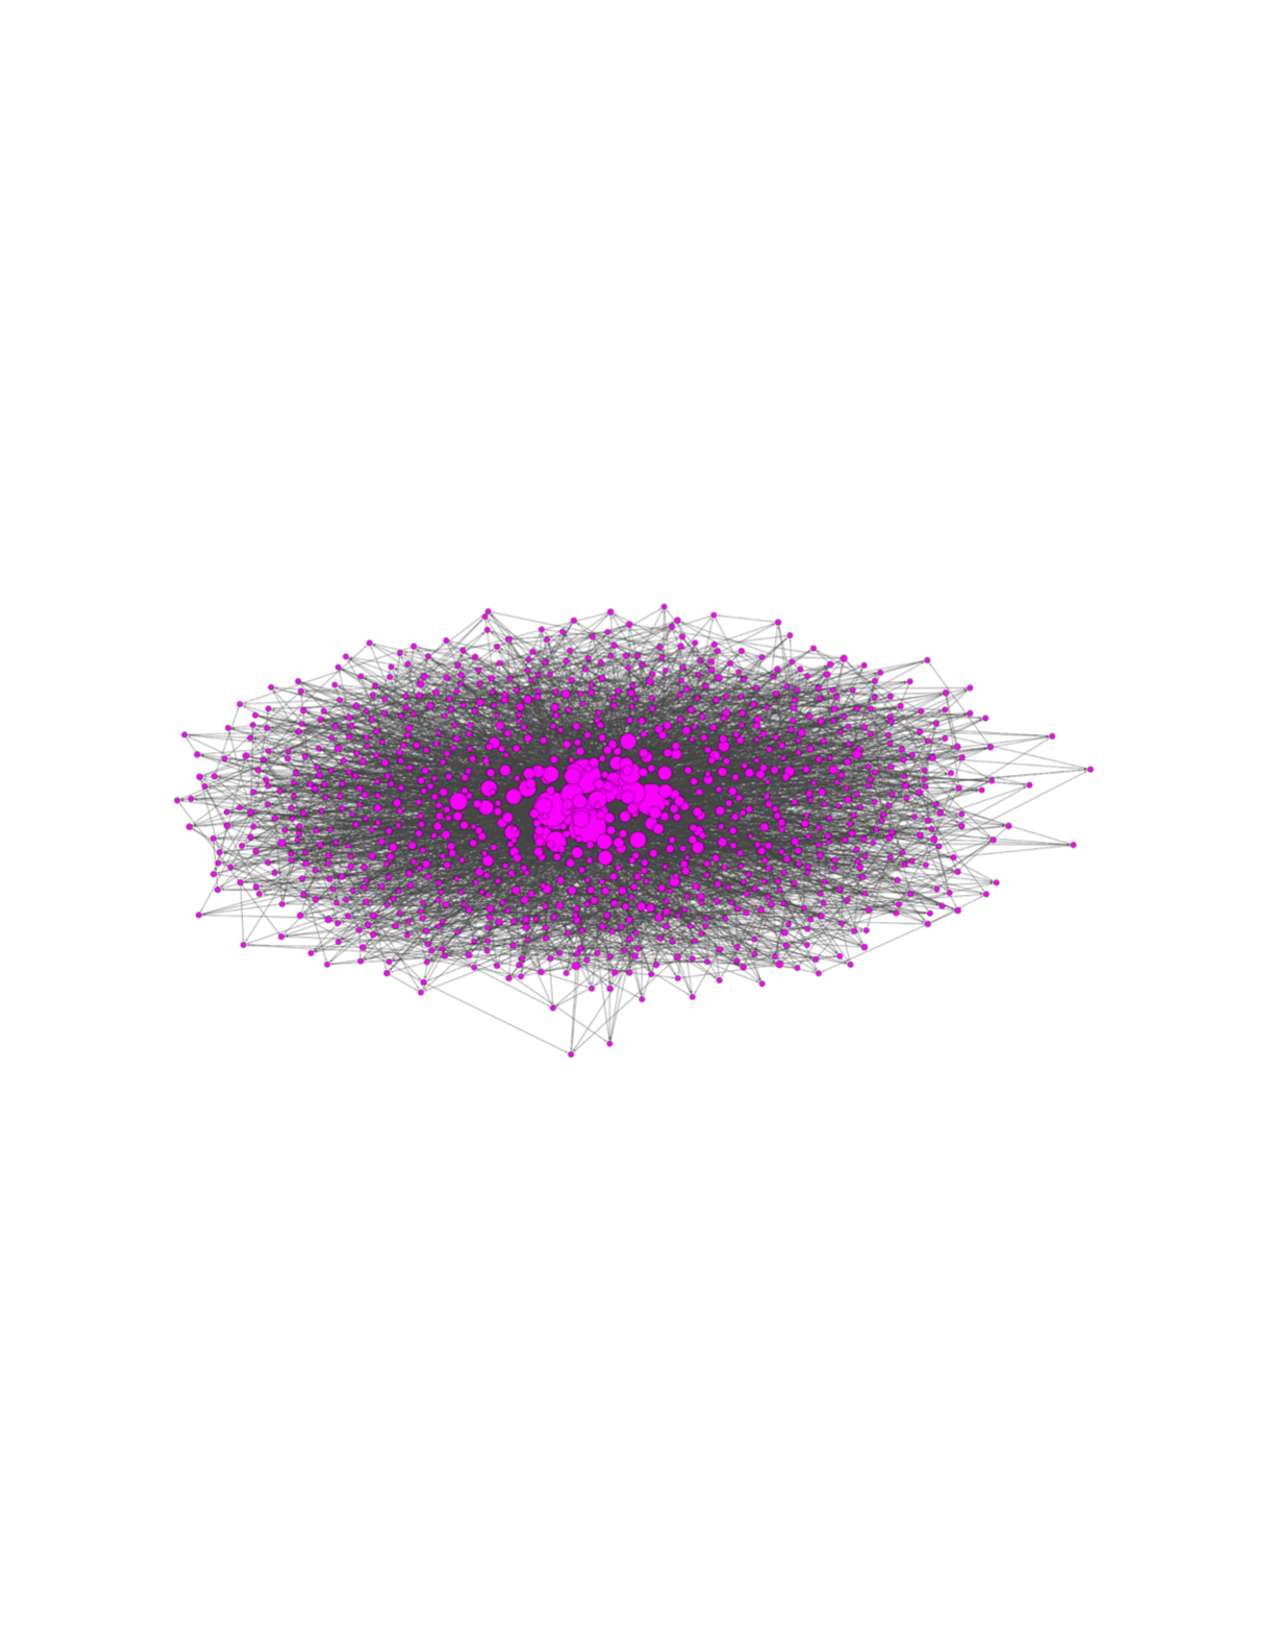
\includegraphics[scale=0.3]{figures/graph_nodes.pdf}
%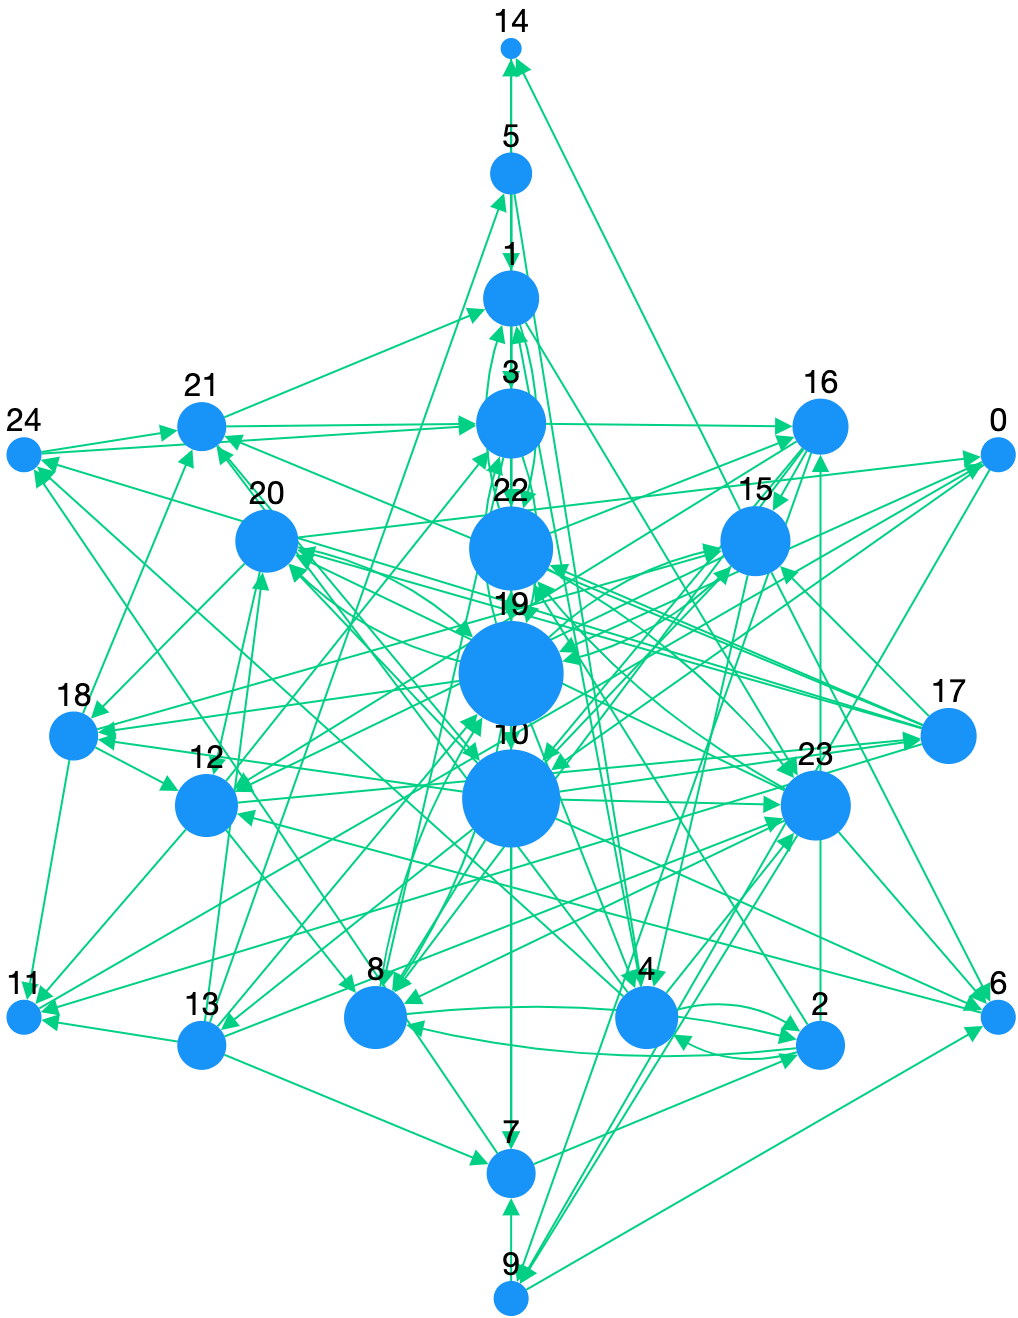
\includegraphics[scale=0.06]{figures/gnm-25-100_pngraph.png} 

\end{minipage}
\hfill
\begin{minipage}{0.3\linewidth}

%Client-side rendering

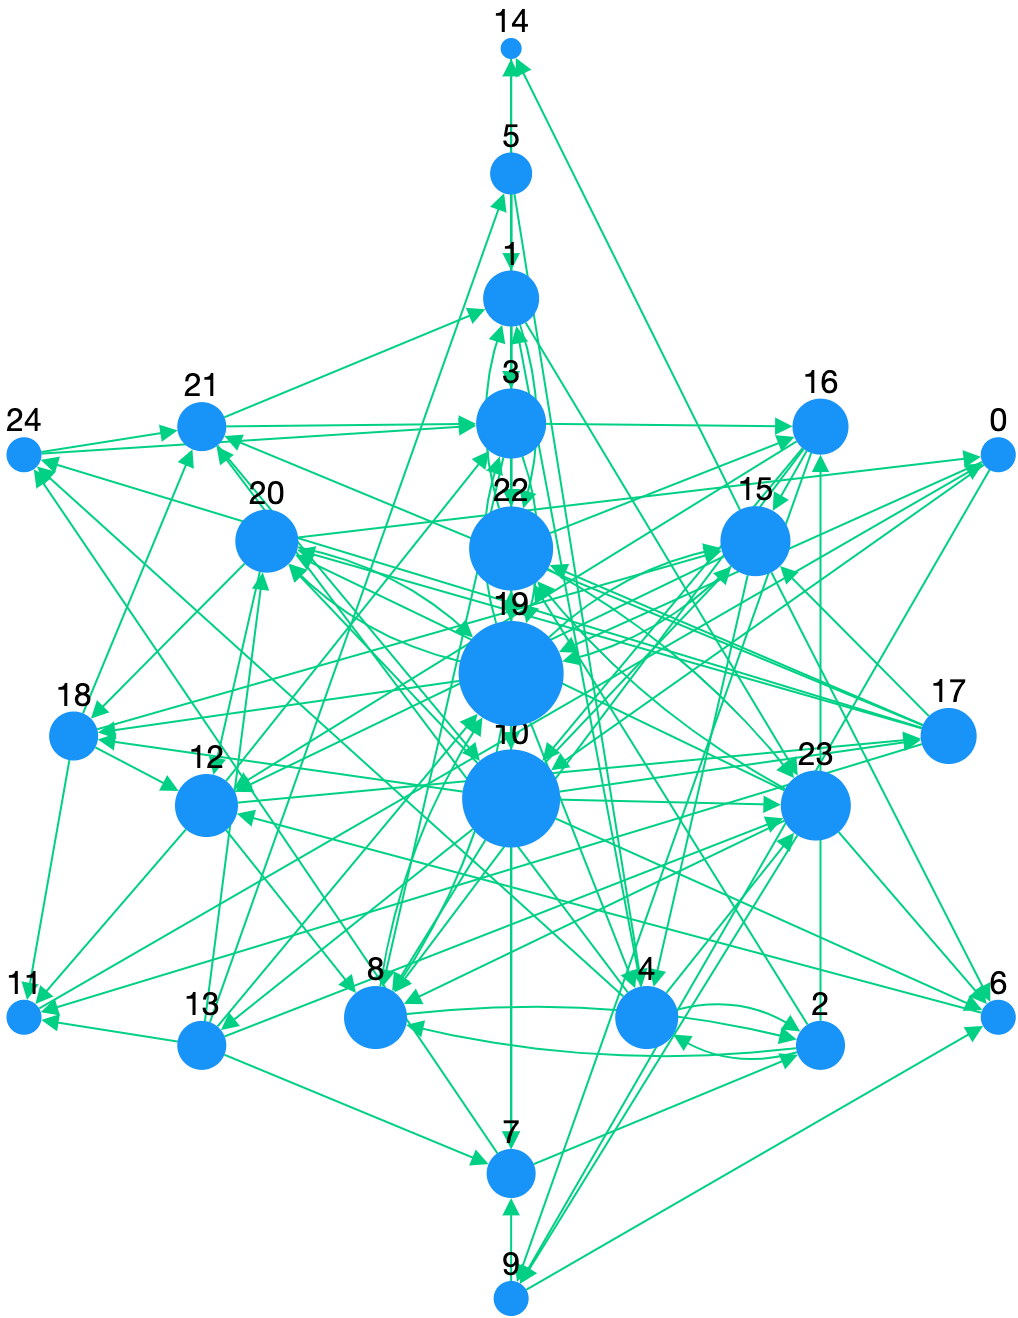
\includegraphics[trim = -4.0in 0in 0in 0in, clip, scale=0.06]{figures/gnm-25-100_pngraph.png} 

\end{minipage}

%\vspace{5mm}
%pngraph visualization

%\begin{center}
%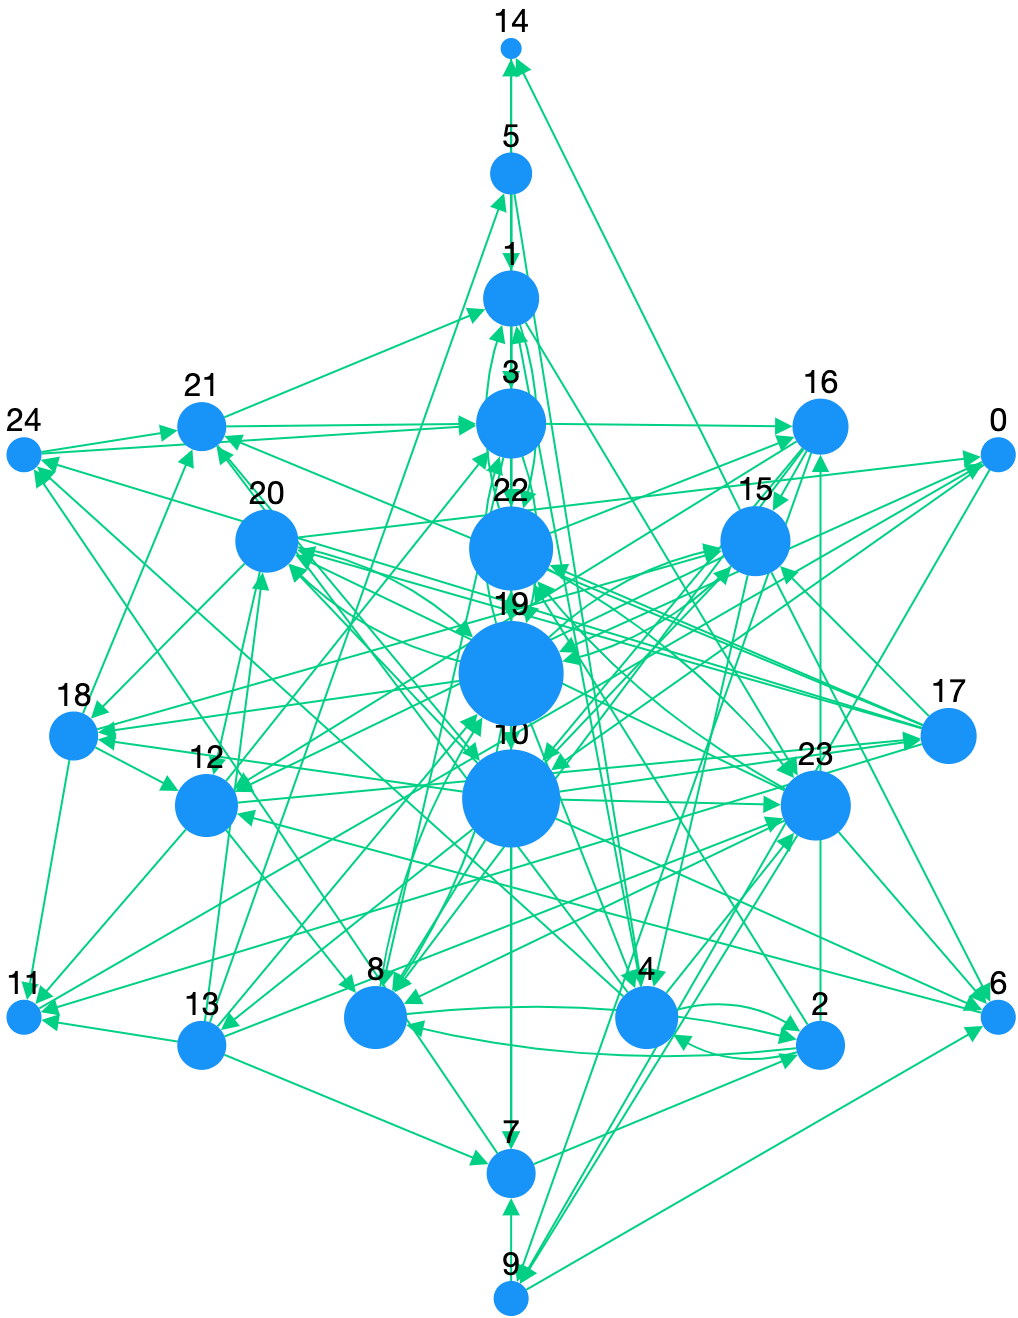
\includegraphics[scale=0.12]{figures/gnm-25-100_pngraph.png} 
%\end{center}

\vspace{0.3in}


\begin{minipage}{0.35\linewidth}
Simulation results palette

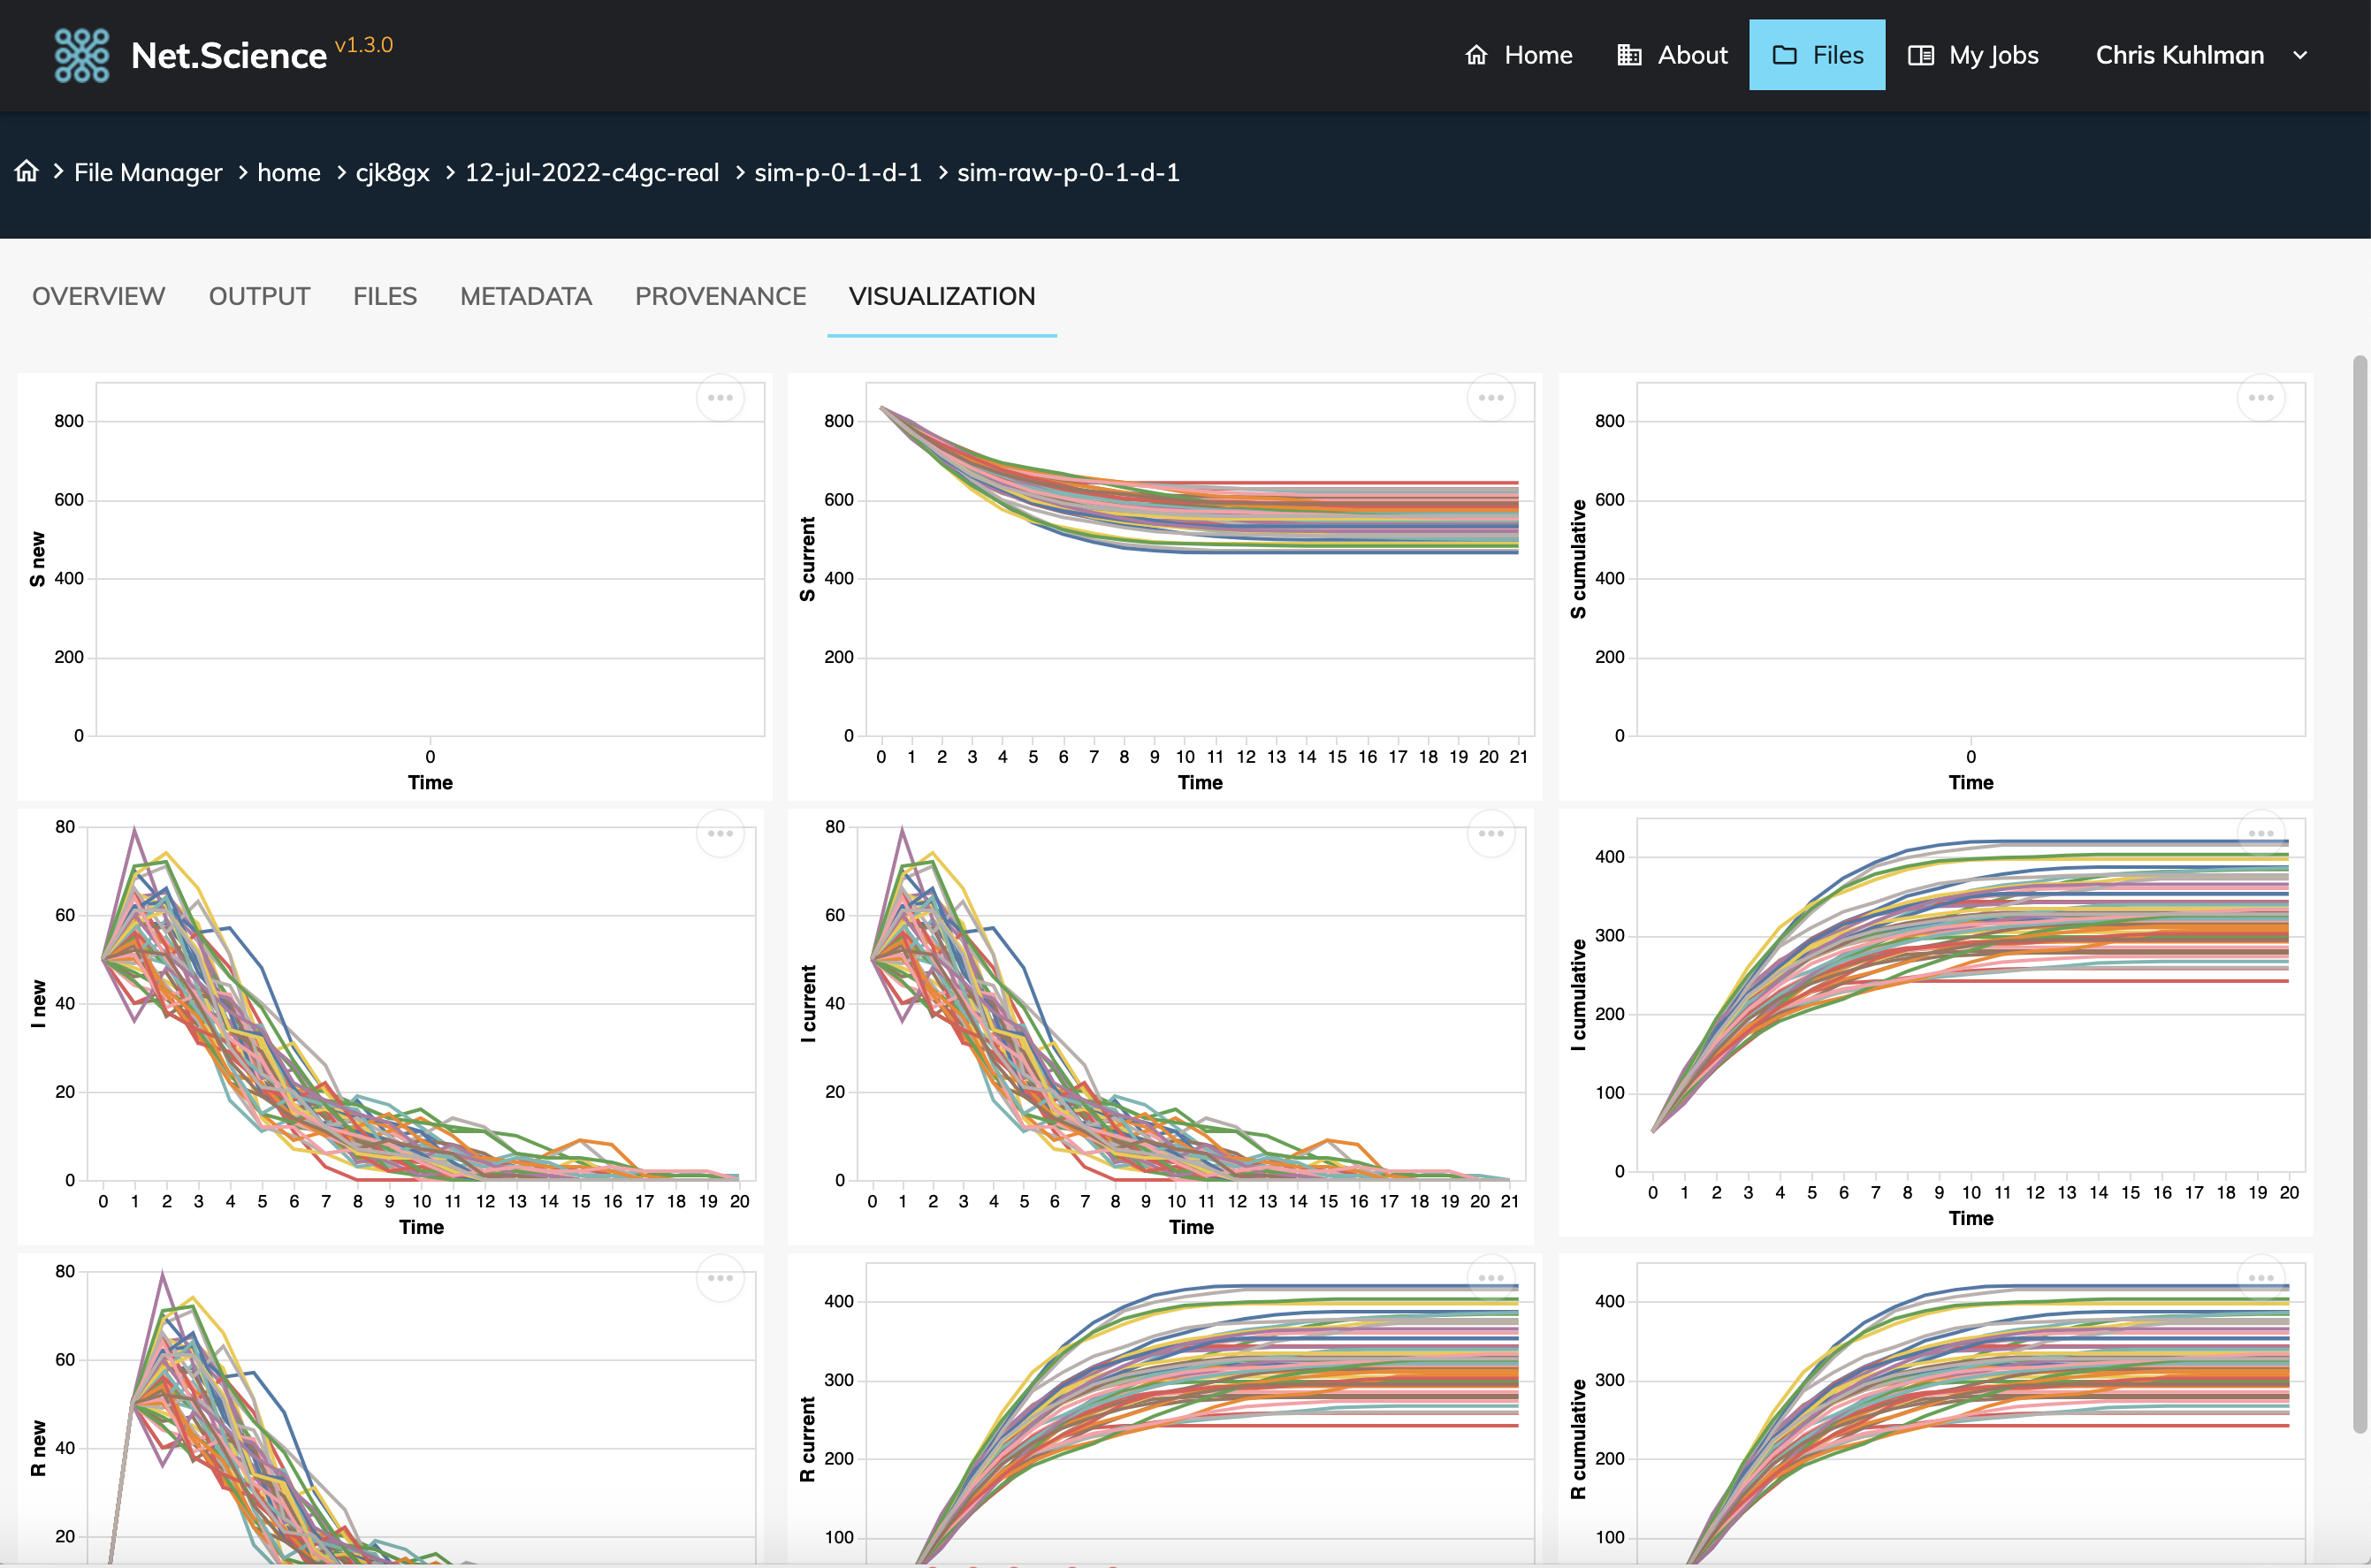
\includegraphics[scale=0.07]{figures/sim_results_pallet} 
\end{minipage}
%\hfill
\hspace{0.1in}
\begin{minipage}{0.36\linewidth}

Discovered graph\newline metadata

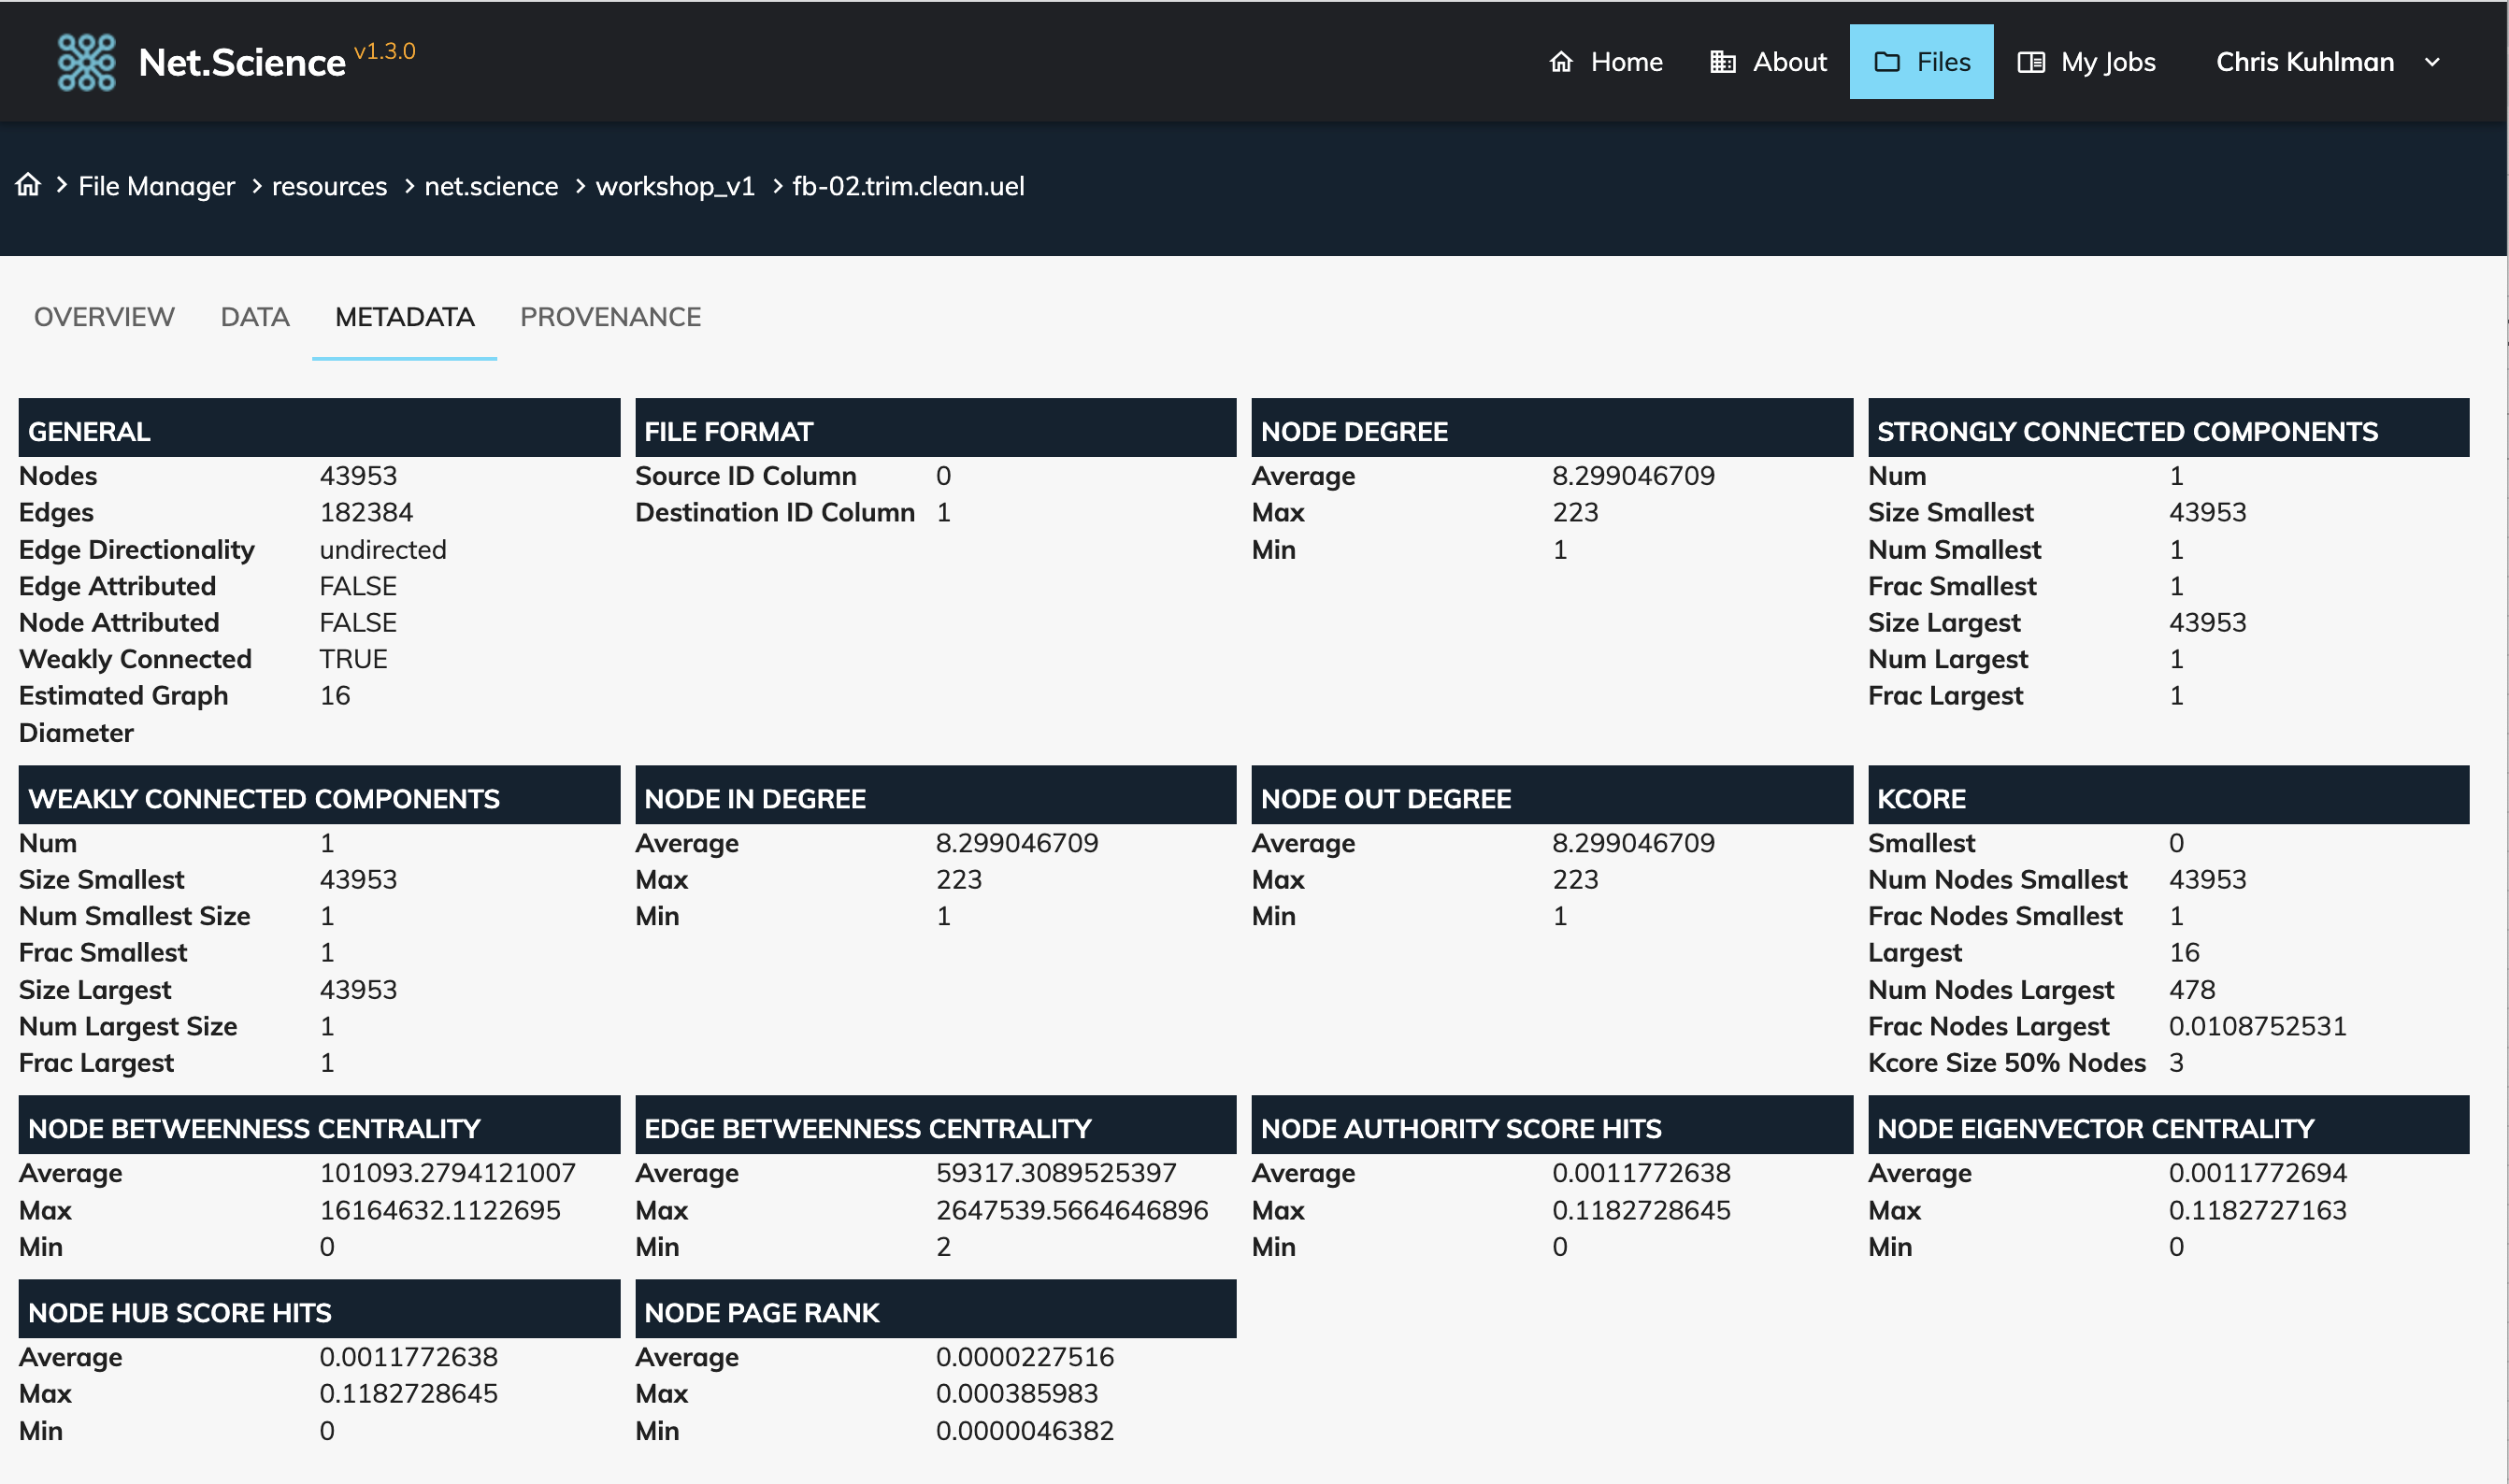
\includegraphics[scale=0.06]{figures/graph_discovered_metadata.png} 
\end{minipage}
%\hfill
\hspace{0.1in}
\begin{minipage}{0.21\linewidth}

Job provenance

%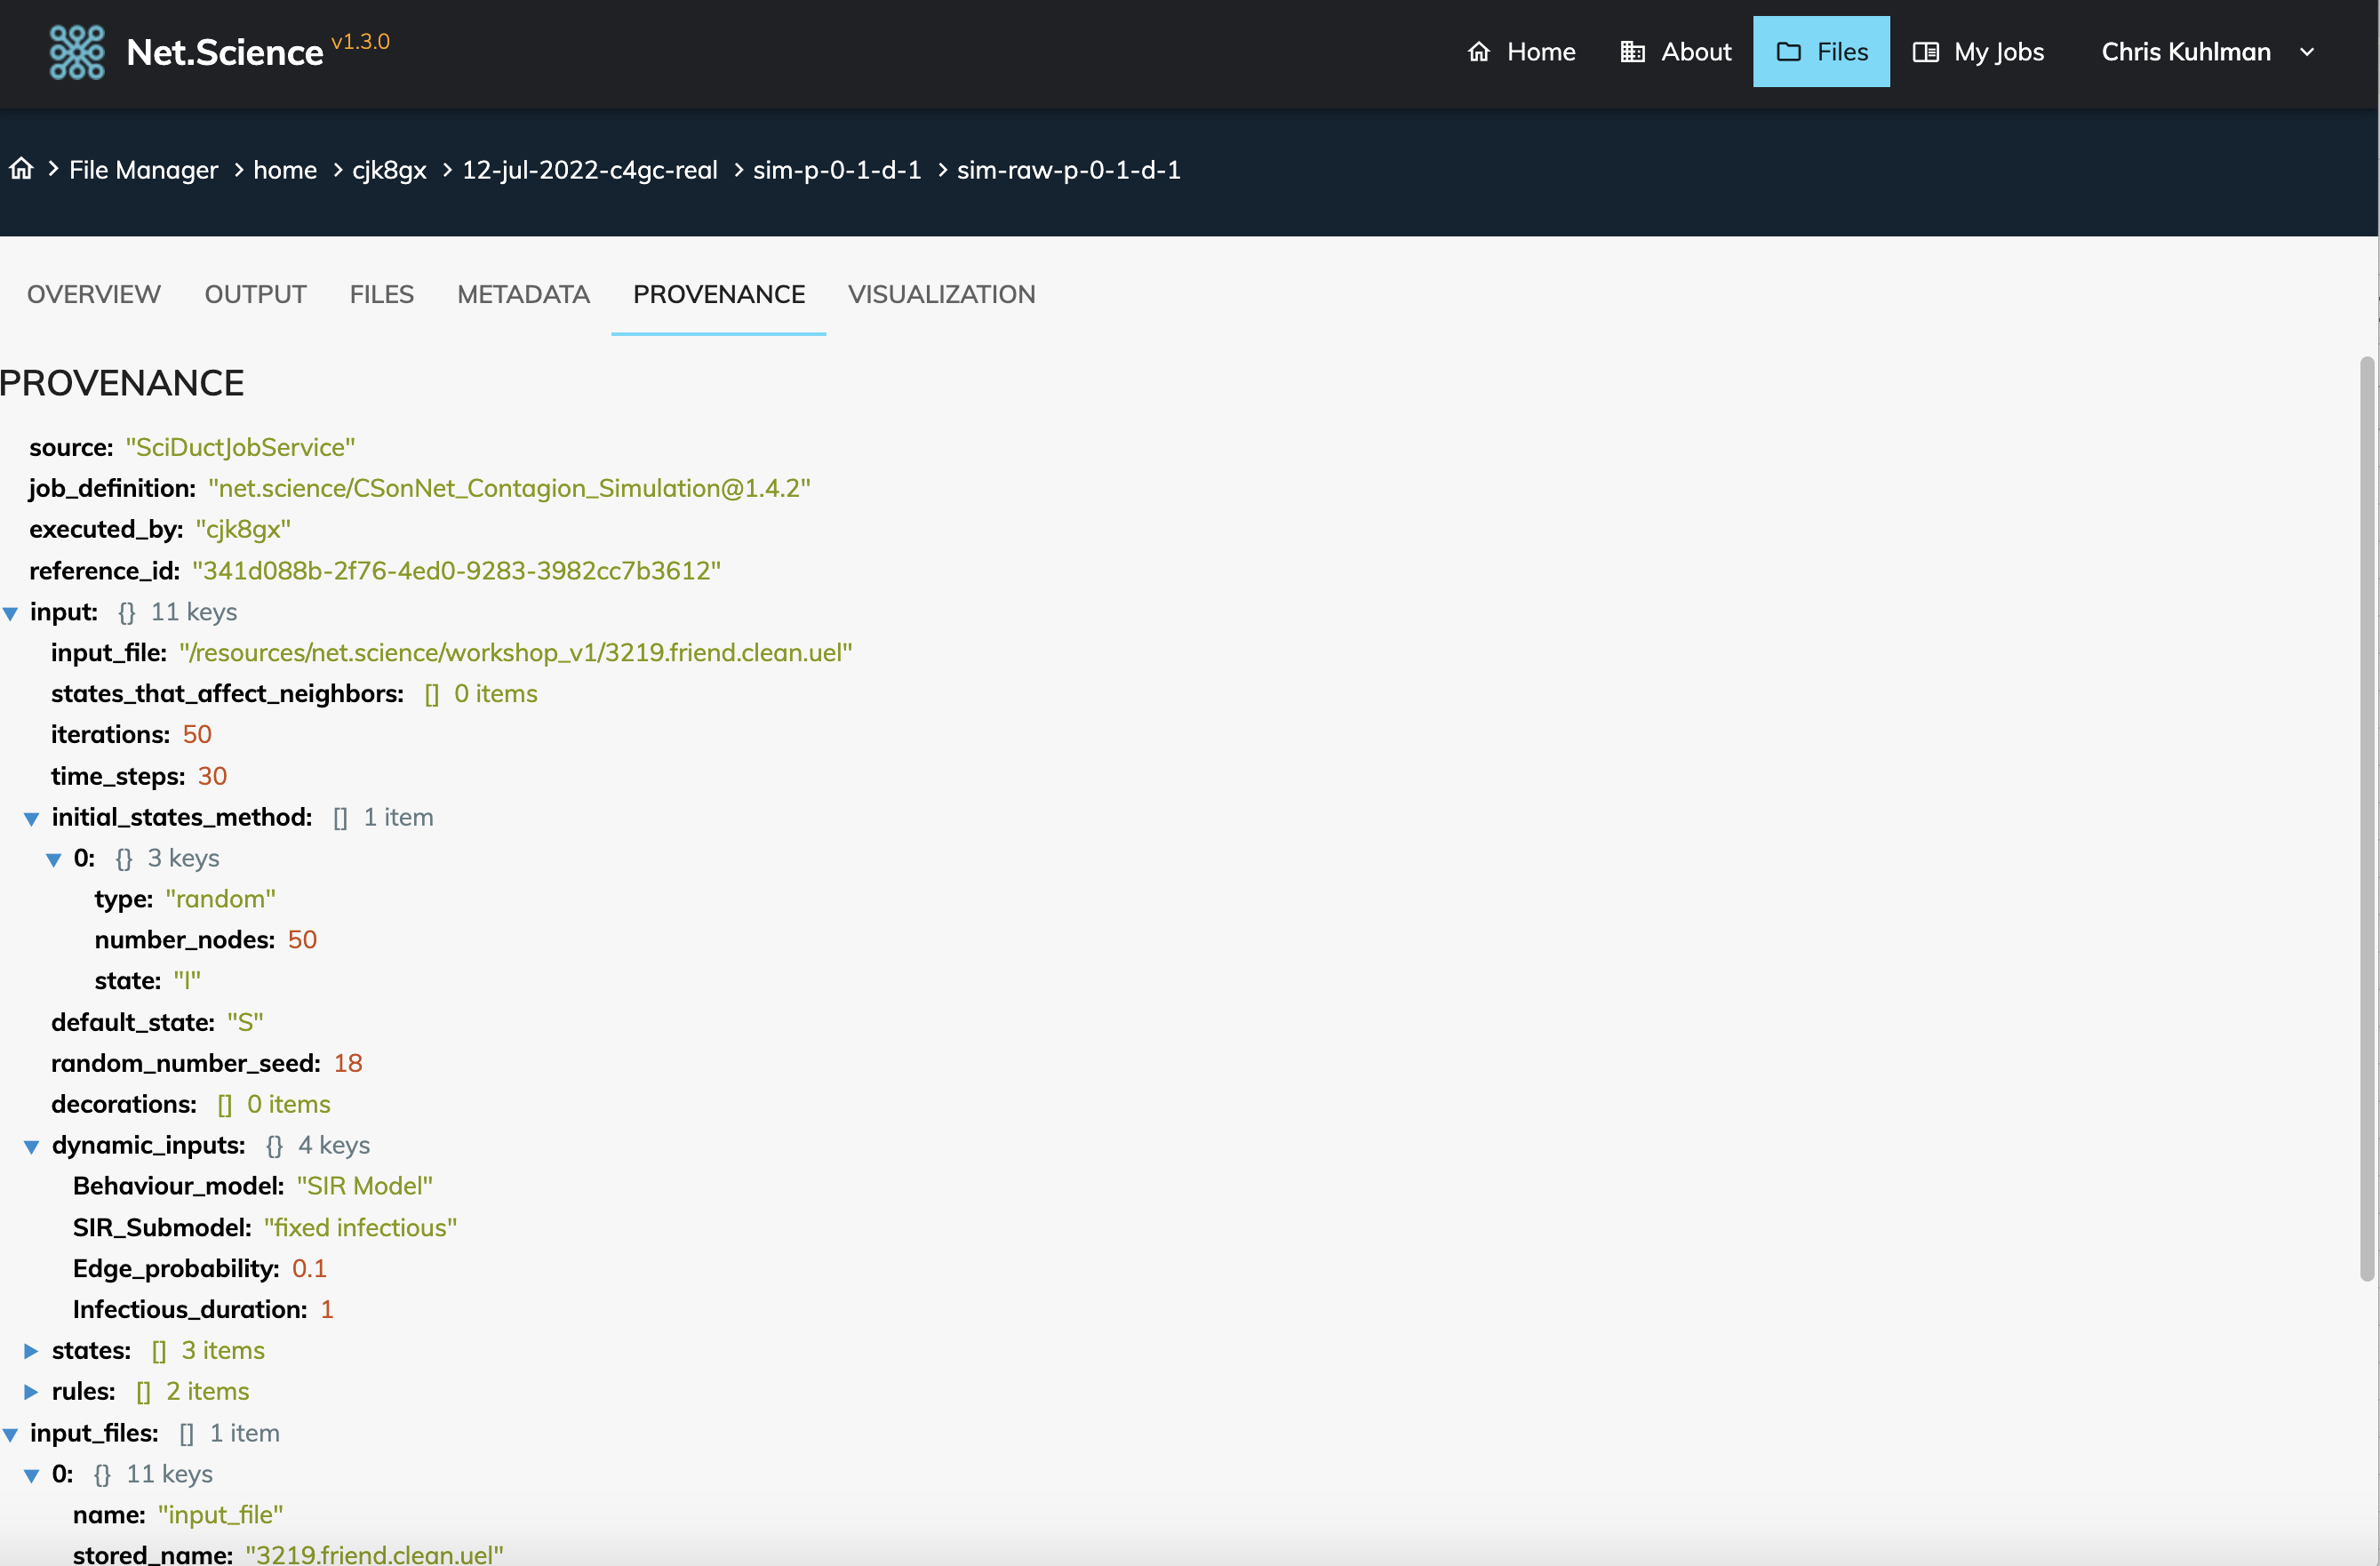
\includegraphics[scale=0.08]{figures/provenance.png} 
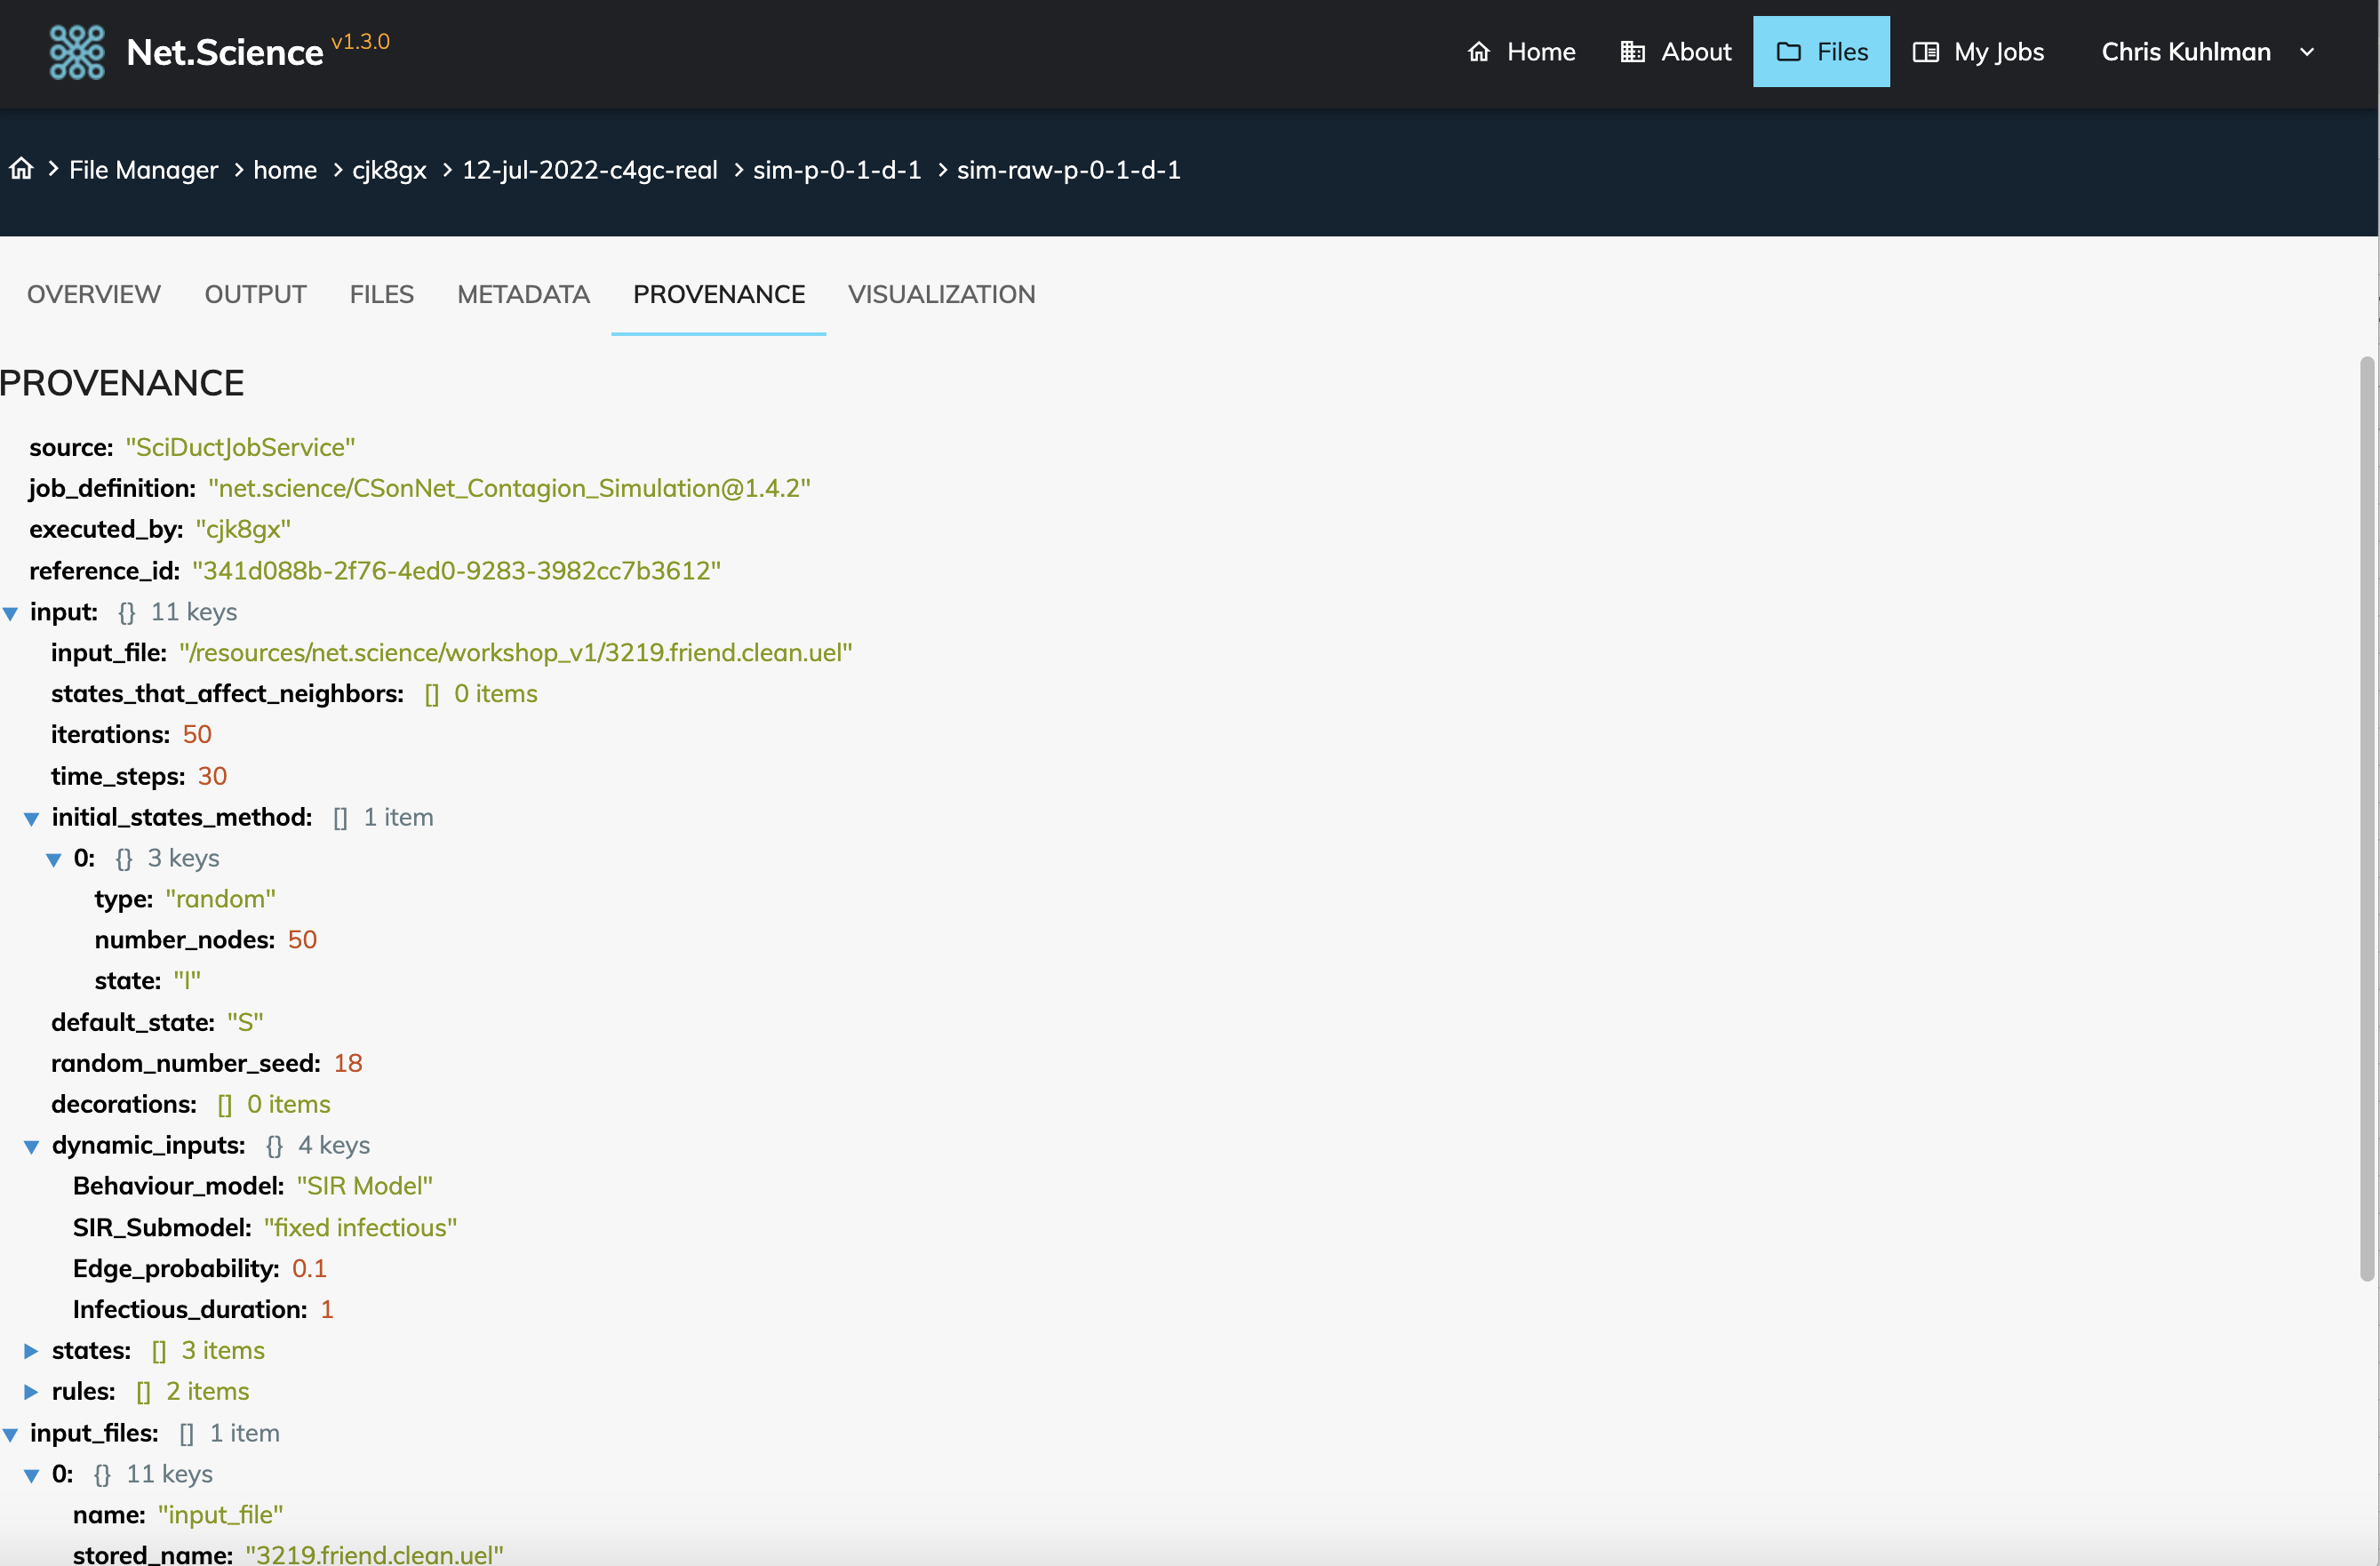
\includegraphics[trim = 0in 0in 10in 0in, clip, scale=0.08]{figures/provenance.png}
\end{minipage}


}

\headerbox{Computational Tasks}
          {name=tasks,column=3,row=0}{

\vspace*{-0.01in}

\begin{center}
\textcolor{blue}{\large\textbf{User Applications: Example CSonNet}}
\end{center}

\vspace*{-0.15in}


\begin{minipage}{0.5\linewidth}
\centering
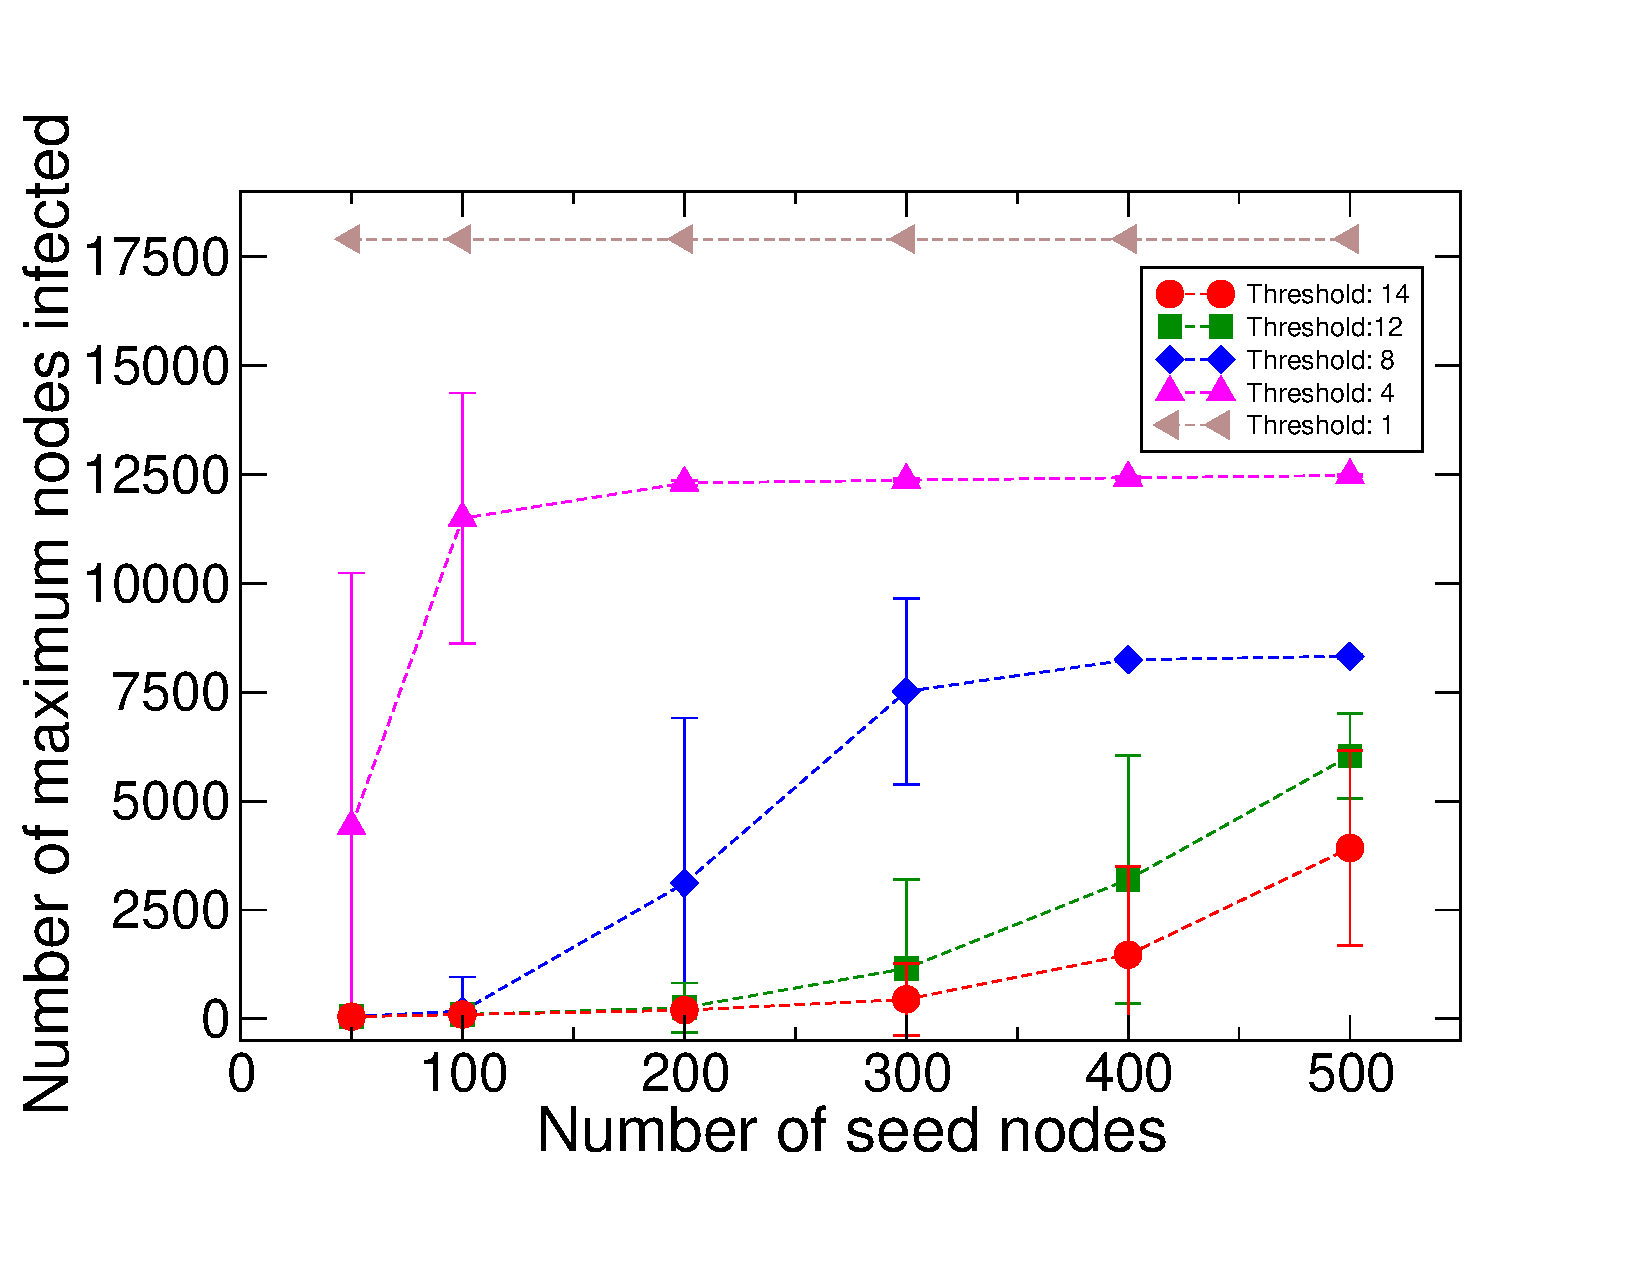
\includegraphics[trim = 0in 0in 0in 0.4in, clip, scale=0.16]{figures/astroph_threshold_cs.pdf} 
\end{minipage}
\hfill
\begin{minipage}{0.5\linewidth}
\centering
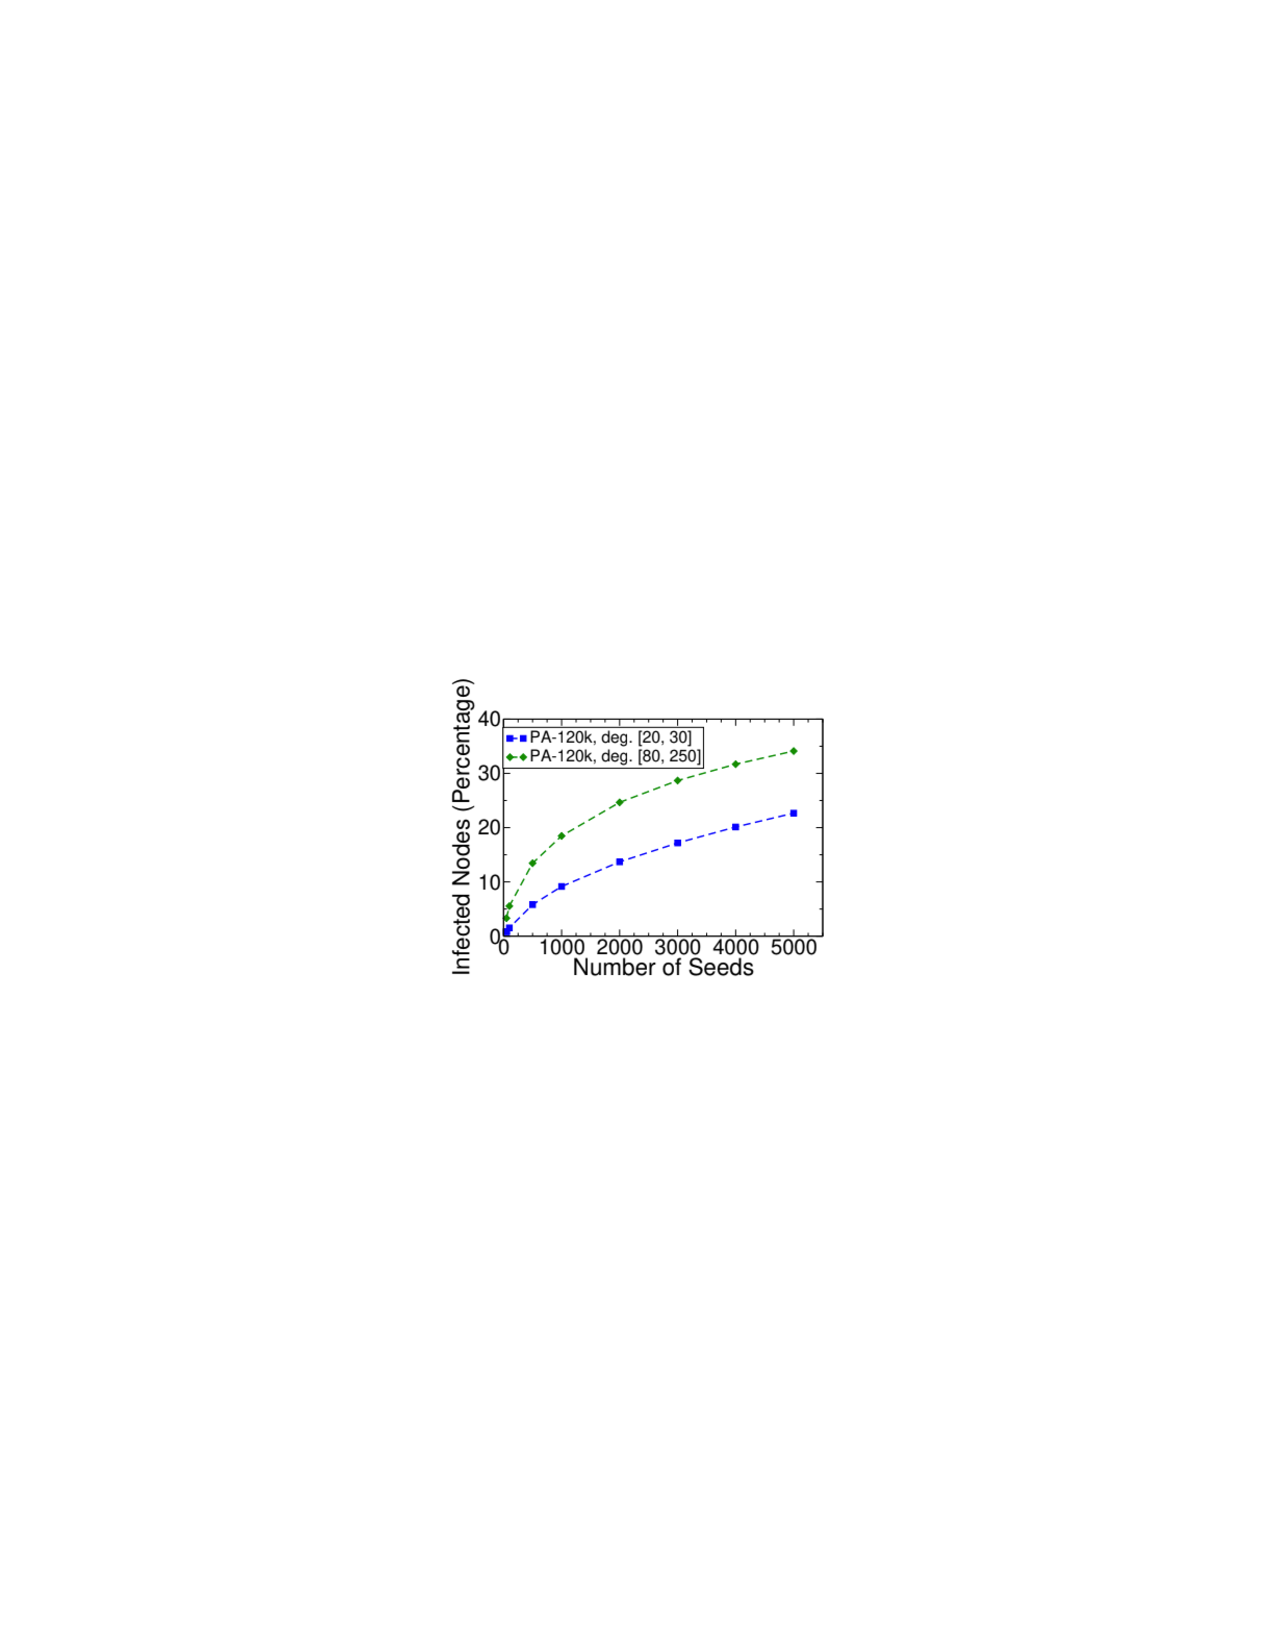
\includegraphics[trim = 0in 0in 0in 0.2in, clip, scale=0.6]{figures/clustering_seed.pdf} 
\end{minipage}
%\hfill
%\begin{minipage}{0.5\linewidth}
%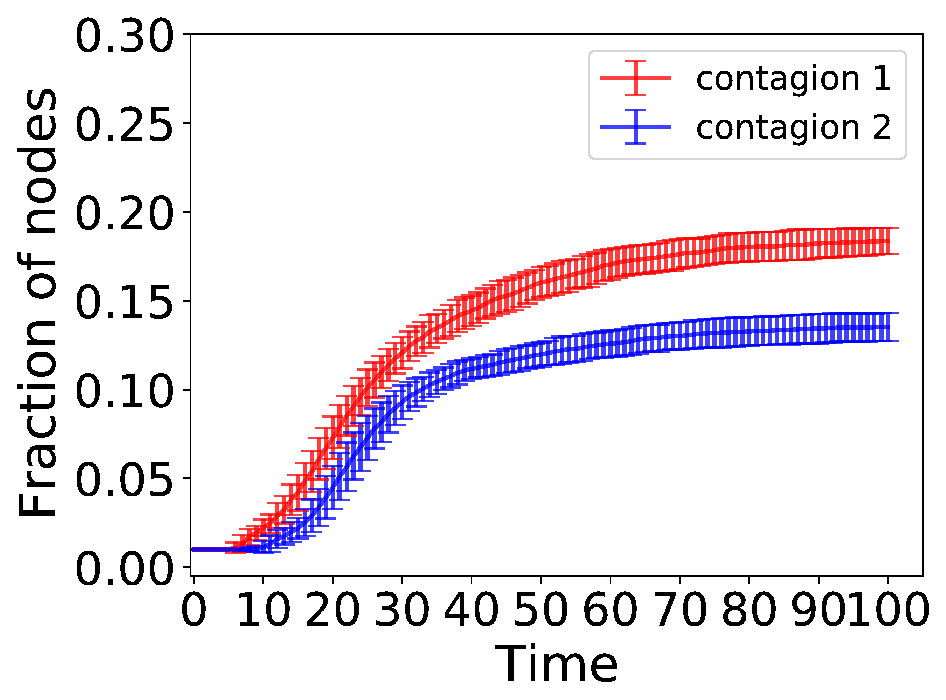
\includegraphics[scale=0.27]{figures/danville_asym_interaction_100ns_fraction_cum_errorbar.eps} 
%\end{minipage}
%\vspace{5mm}
%\hfill
%\begin{minipage}{0.48\linewidth}
%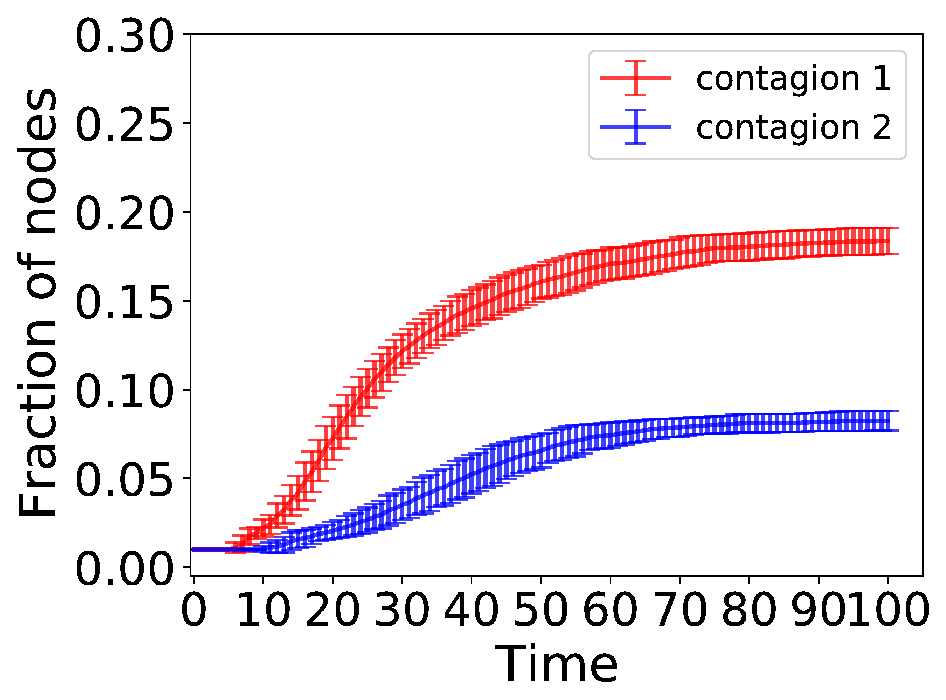
\includegraphics[scale=0.27]{figures/danville_no_interaction_100ns_fraction_cum_errorbar.eps} 
%\end{minipage}


%	\begin{itemize}
%	\item CSONNET (Graph Seeding, Plotting)
%	\item Structural Analysis
%	\item Graph Generation
%	\end{itemize}

\vspace*{-0.2in}


\begin{center}
\textcolor{blue}{\large\textbf{Common Services: Example Graph Transformations}}
\end{center}
\begin{center}
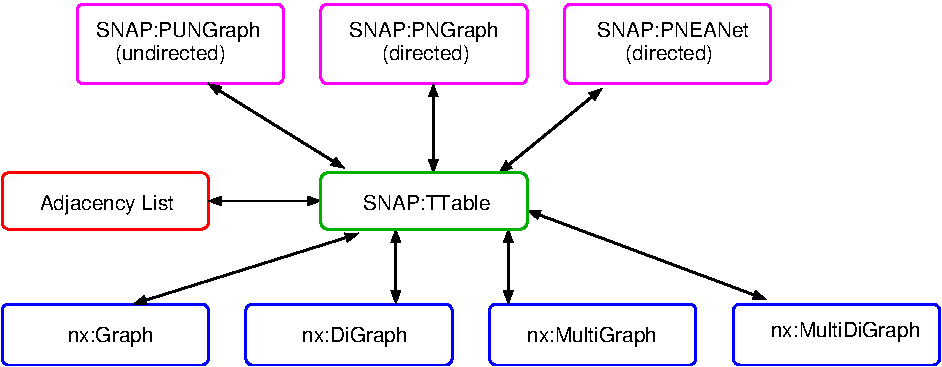
\includegraphics[scale=0.4]{figures/star_trans.pdf}
\end{center}

\hfill
\begin{minipage}{0.45\linewidth}
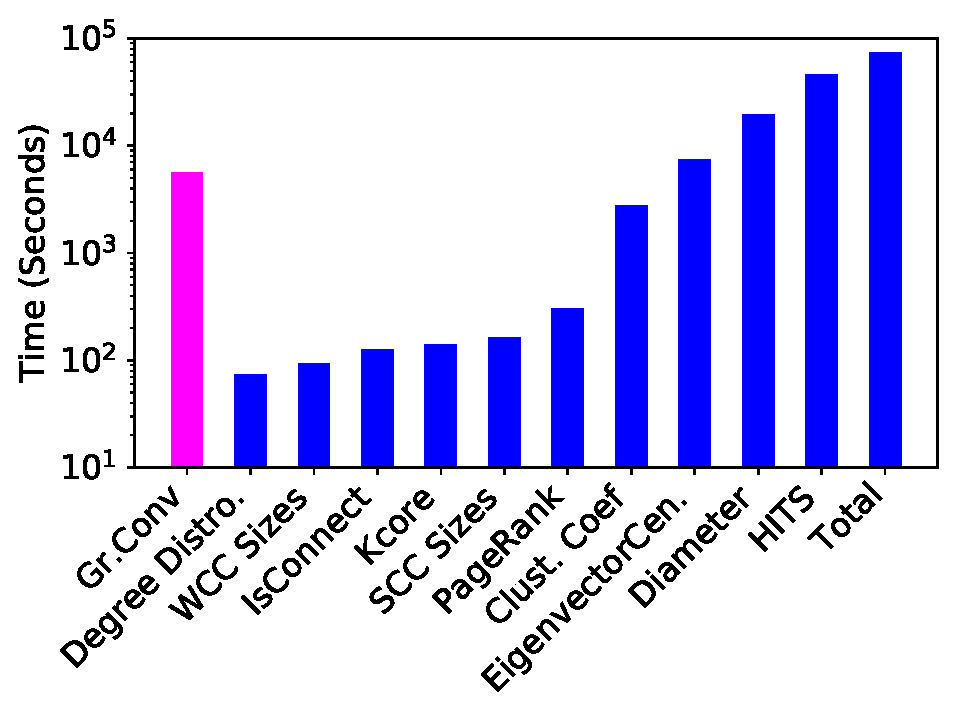
\includegraphics[scale=0.27]{figures/g4_timing.pdf} 
\end{minipage}
\hfill
\begin{minipage}{0.45\linewidth}
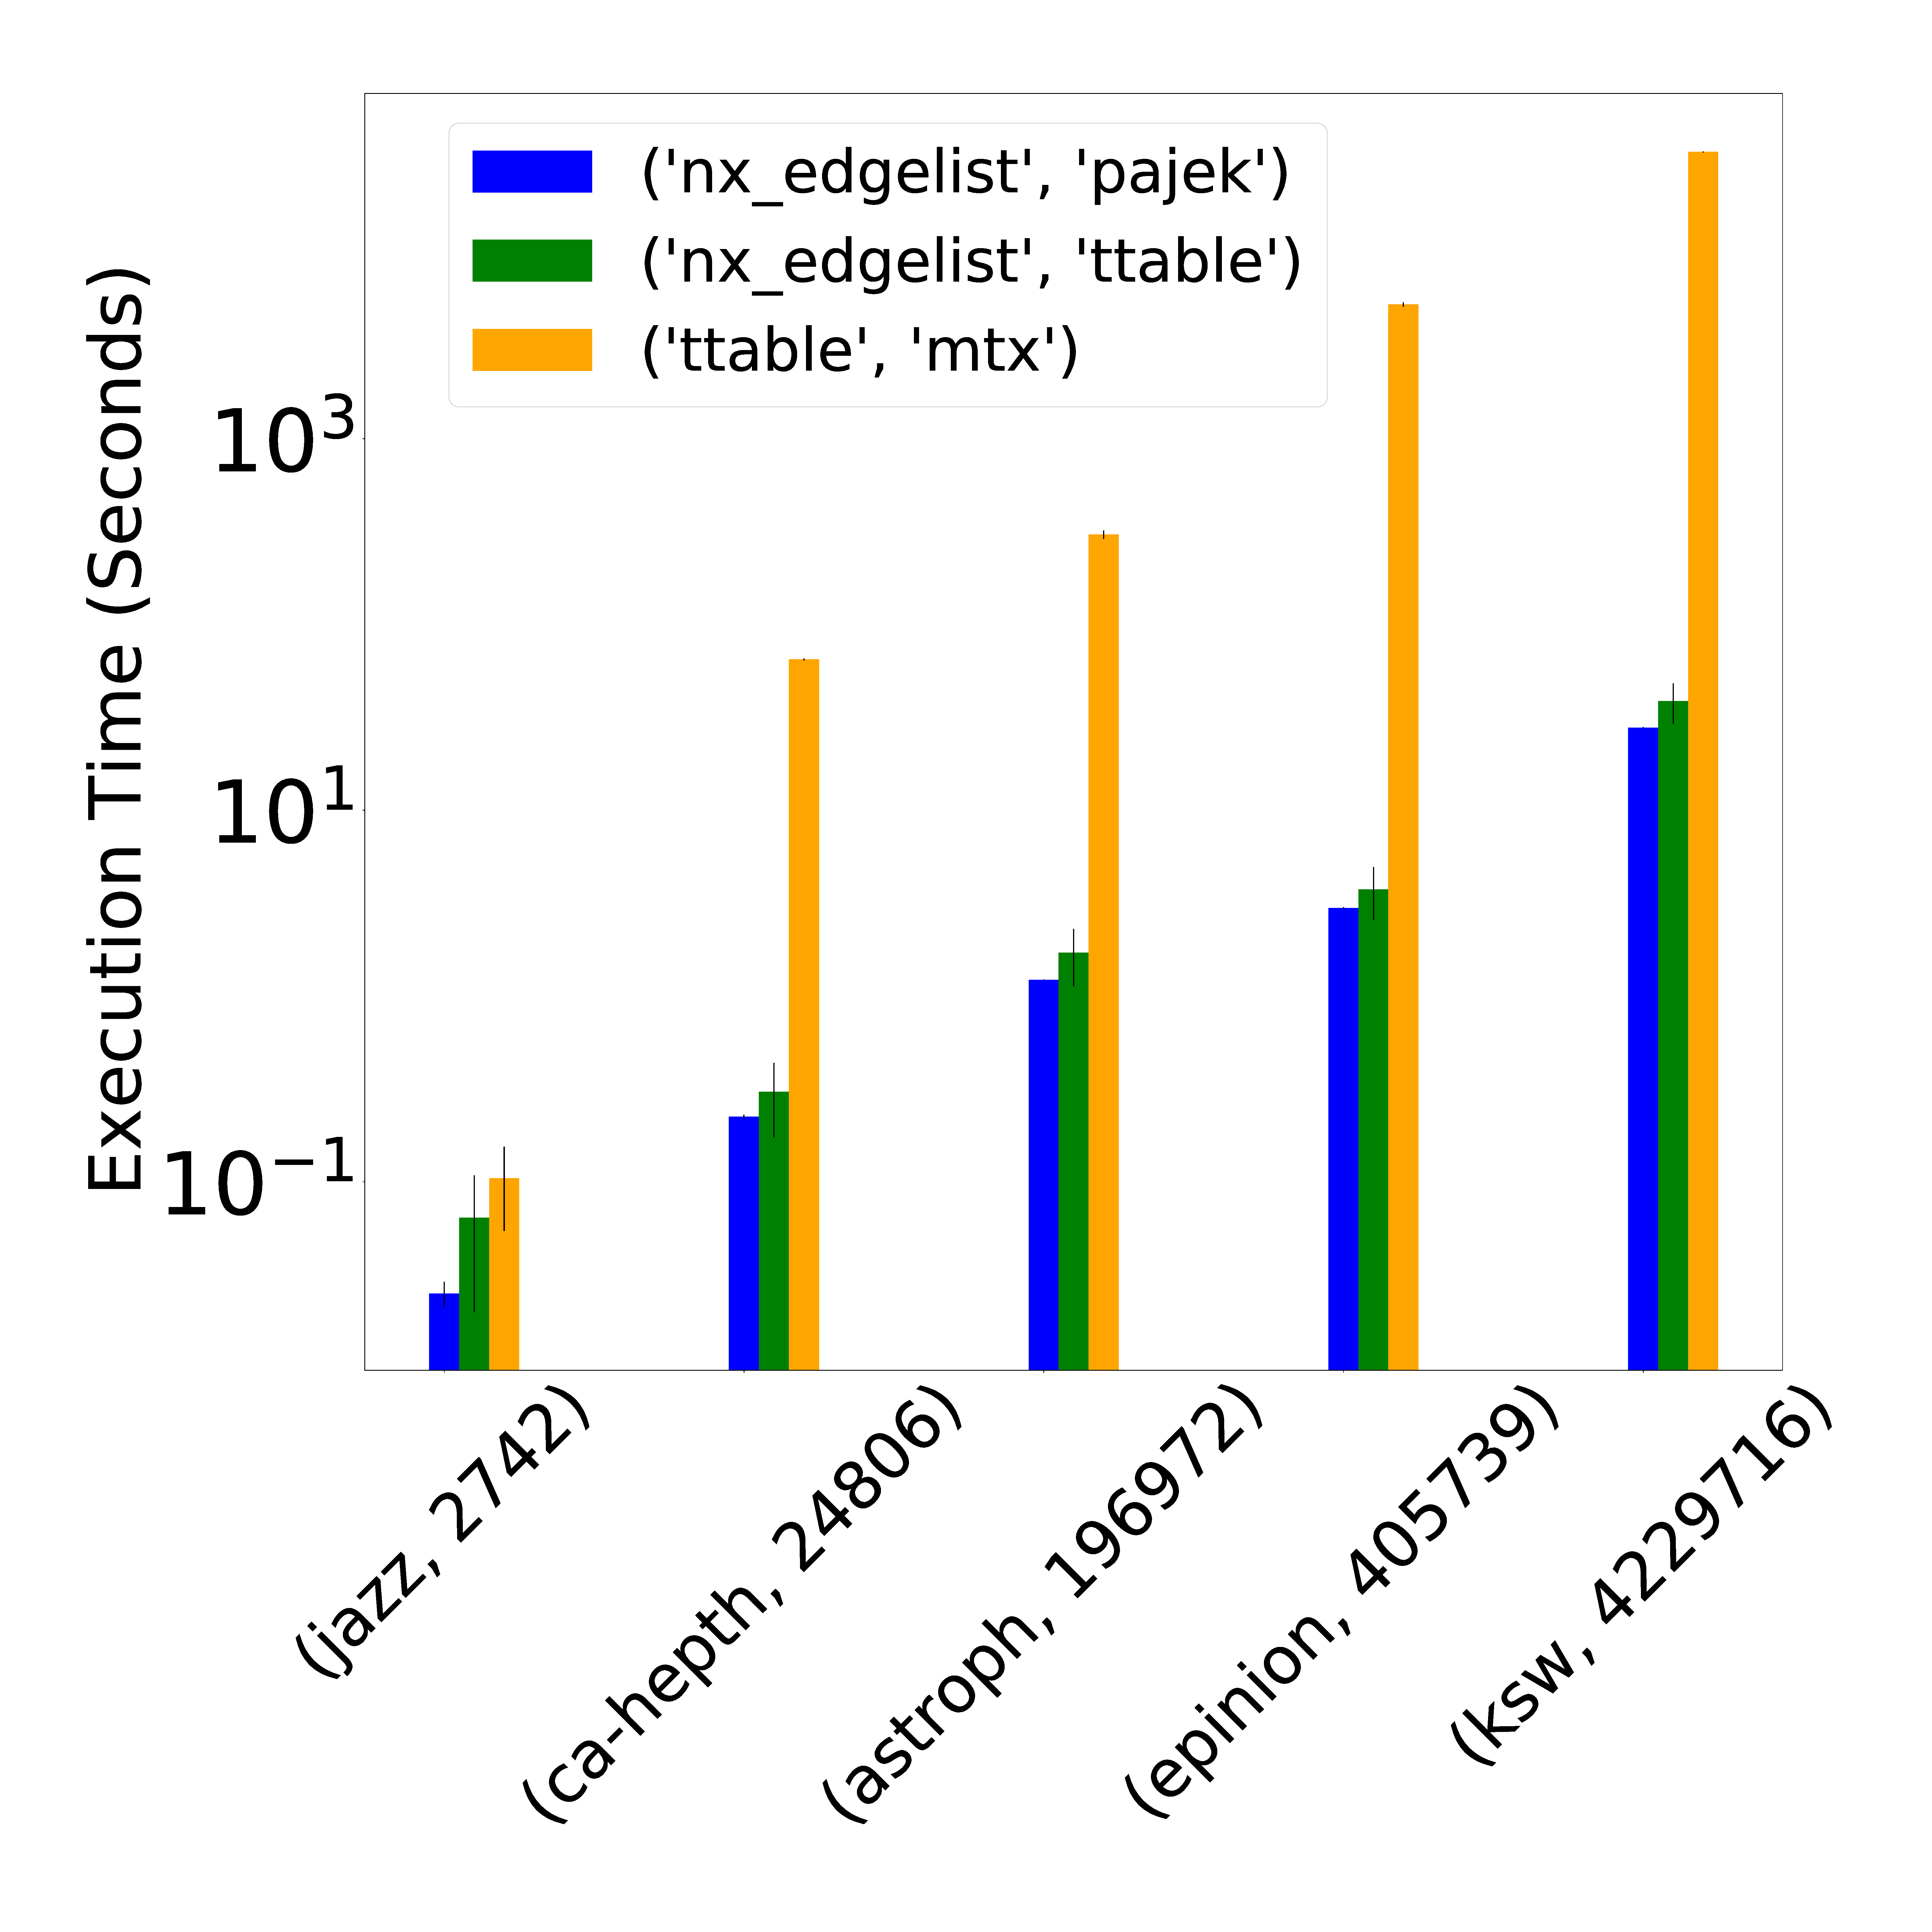
\includegraphics[scale=0.038]{figures/scatter_bar_to_ttable.pdf}
\end{minipage}

}


\headerbox{Outreach and System Usage}
          {name=outreach,column=3,row=2, below=tasks}{
\begin{minipage}[t]{0.48 \textwidth}
%\textbf{Implemented} ($\approx$ 200 total)   \smallskip
\textcolor{blue}{\textbf{System Demos}}
\medskip
\begin{itemize}[leftmargin=*,noitemsep,topsep=0pt]
    \item 3 ACM/IEEE conferences  \smallskip
    \item 2 graduate courses   \smallskip 
    \item 1 undergraduate course  \smallskip
    \item 2 short courses  \smallskip
    \item 1 C4GC undergraduate program  \smallskip
    \item \textcolor{red}{XXXX} other 
\end{itemize}
\end{minipage}
\quad
\begin{minipage}[t]{0.48 \textwidth}
%\textbf{In progress}
\textcolor{blue}{\textbf{Course Use}}\
  \medskip
\begin{itemize}[leftmargin=*,noitemsep,topsep=0pt]
    \item 2 graduate network science    \smallskip
    \item 1 undergraduate algorithms   \smallskip
    \item 1 short course network science   \smallskip
    \item \textcolor{magenta}{1 systems course}  \smallskip
    \item \textcolor{magenta}{1 security short course}  \smallskip
    \item \textcolor{magenta}{1 databases}  \smallskip
    \item \textcolor{magenta}{1 Data Science Capstone}
\end{itemize}
\end{minipage}\\
\quad
%
\begin{minipage}[t]{0.48 \textwidth}
\textcolor{blue}{\textbf{Usage Statistics}}
\medskip
\begin{itemize}[leftmargin=*,noitemsep,topsep=0pt]
    \item 3 ACM/IEEE conferences  \smallskip
    \item 2 graduate courses   \smallskip 
    \item 1 undergraduate course  \smallskip
    \item 2 short courses  \smallskip
    \item 1 C4GC undergraduate program
\end{itemize}
\end{minipage}
\quad
\begin{minipage}[t]{0.48 \textwidth}
%\textbf{In progress}
\textcolor{blue}{\textbf{Course Use}}\
  \medskip
\begin{itemize}[leftmargin=*,noitemsep,topsep=0pt]
    \item 2 graduate network science    \smallskip
    \item 1 undergraduate algorithms   \smallskip
    \item 1 short course network science   \smallskip
    \item \textcolor{magenta}{1 systems course}  \smallskip
    \item \textcolor{magenta}{1 security short course}
    \item \textcolor{magenta}{1 databases}
\end{itemize}
\end{minipage}
}


\headerbox{Acknowledgments}
          {name=Ack,column=3,row=3,below=outreach}{
{\footnotesize
This work was supported by
NSF Grants OAC-1916805 (CINES) and CMMI-1916670 (CRISP 2.0),
University of Virginia Strategic Investment Fund award
number SIF160.
}
}

\headerbox{Contact Persons}
          {name=Contact,column=3,row=4,below=Ack}{
{\footnotesize
{Madhav V. Marathe~ (\textcolor{green}{\textbf{\texttt{marathe@virginia.edu}}})}\\
{Chris J. Kuhlman~ (\textcolor{green}{\textbf{\texttt{cjk8gx@virginia.edu}}})}
}}

\end{poster}



\end{document}
